\documentclass{TeFlon}
%%%%%%%%%%%%%%%%%%%%%%%%%%%%
%        TeFloN X
%        -PASCAL-
%%%%%%%%%%%%%%%%%%%%%%%%%%%

\begin{document}
% PARA CAMBIAR EL TITULO SUPERIOR DENTRO DE CADA PAGINA ES EL ULTIMO PARAMETRO
\incorporarDatos{no}{UCM}{informática}{Ingeniería de Software}{\textit{Dirigido por}\\ Antonio Sarasa Cabezuelo\vspace{2mm}}{2021--2022}{Madrid}{David Fernández Alejo\\ Vitaliy Savchenko\\ Carlos Segundo Nieto\\ Víctor Velasco Arjona}{Aplicación Android para gestionar la dieta de un deportista}

%%%%%%%%%%%%%%%%%%%%%%%%%%%%%%%%%%%%%%%%%%% Parte 1 - TFG
\tituloTFG
\begin{titlepage}
\vspace{4cm}
\centering
{\textsf{\huge  \textbf{Aplicación Android para gestionar la dieta de un deportista}}}

\vspace{0.3cm}

{\textsf{\large \textbf{Android application to manage the diet of an athlete} }}

\vspace{7cm}
\textit{Memoria que se presenta para el Trabajo de Fin de Grado}\\
\vspace{5mm}
{\large \textbf{ David Fernández Alejo\\ Vitaliy Savchenko\\ Carlos Segundo Nieto\\ Víctor Velasco Arjona}}

\vspace{2cm}
\textit{Dirigido por}\\
\vspace{5mm}
{\bfseries Antonio Sarasa Cabezuelo}

\vfill

\textbf{{Departamento de Sistemas Informáticos y Computación\\
Facultad de Informática\\
Universidad Complutense de Madrid}}\\
\vspace{5mm}
\textbf{Madrid, 2022}
\end{titlepage}
\fantasma
\newpage
\chapter*{Agradecimientos}
\noindent

Agradecemos a nuestras familias el apoyo incondicional durante la realización del trabajo y a todas las personas que nos han dado una opinión crítica de la aplicación, ayudando a mejorarla.
\newpage
\chapter*{Resumen}
\noindent

% En este proyecto se describe con el mayor detalle posible una aplicación destinada al ámbito de la ingeniería del software. Al hablar con muchos deportistas se puede llegar a una conclusión de que el principal problema a la hora de realizar algún deporte o destinar parte del tiempo en realizar cualquier tipo de ejercicio es la dificultad que tiene la gente en proponerse una dieta para cumplir sus metas. El objetivo de este proyecto consiste en solventar este problema mediante la realización de una red de deportistas mediante el uso de la tecnología móvil en la que poder crear, observar y publicar dietas para que todos los usuarios registrados en la plataforma puedan realizarlas y seguirlas con una mayor facilidad posible.

% Esta Herramienta se ha desarrollado mediante la tecnología Android que mediante el uso de dos roles, administrador y deportista, serán capaces de desarrollar la actividad para la que se ha llevado a cabo. El/los administrador/es serán los encargados de gestionar todo el tema de usuarios, y tendrán todos los permisos necesarios para editar, crear y borrar cualquier elemento insertado en la aplicación mientras que los deportistas serán los miembros que disfrutaran de la aplicación permitiéndoles crear, y seguir las dietas necesarias para lograr su objetivo.

En este proyecto se describe la especificación de requisitos, diseños e implementación de una aplicación Android para la gestión de dietas para deportistas.

Todo deportista necesita complementar su actividad física con una dieta saludable. En este sentido, un problema bastante habitual es ser constante en el seguimiento de la misma. Es por ello que este trabajo se ha tratado de resolver este problema proporcionado una aplicación orientada específicamente a gestionar dietas y a facilitar al usuario el seguimiento de las mismas. La aplicación ofrece al usuario la posibilidad de crear y gestionar una serie de dietas para su seguimiento. También se brinda la posibilidad de publicar las dietas creadas por un usuario, las cuales serán visibles por otros usuarios, creando así una red de personas que pueden comentar y valorar las dietas que siguen, para dejar constancia de su eficacia y ayudar con ello al resto de personas que usan la aplicación.

Durante el seguimiento de una dieta, el usuario puede introducir la cantidad consumida de cada uno de los alimentos que componen la dieta, generando un registro de la ingesta calórica por cada día de la semana. Como complemento a todo ello, también se puede introducir la cantidad de pasos caminados durante cada día, así como el peso para que el usuario pueda ver una representación gráfica del progreso.


\begin{center}
    \textbf{Palabras clave}\\
    Android, Spring, sports, API, Node.js
\end{center}

\newpage
\chapter*{Abstract}
\noindent

% This project describes in as much detail as possible an application for the field of software engineering. When talking to many sportsmen and sportswomen, it can be concluded that the main problem when it comes to doing sports or spending part of their time doing any kind of exercise is the difficulty people have in setting a diet to meet their goals. The aim of this project is to solve this problem by creating a network of athletes through the use of mobile technology in which they can create, observe and publish diets so that all registered users on the platform can perform and follow them as easily as possible.

% This tool has been developed using Android technology that through the use of two roles, administrator and athlete, will be able to develop the activity for which it has been carried out. The administrator/s will be in charge of managing all the users, and will have all the necessary permissions to edit, create and delete any element inserted in the application while the athletes will be the members who will enjoy the application allowing them to create and follow the necessary diets to achieve their goal.

This project describes the requirements specification, designs and implementation of an Android application for diet management for athletes.

Every athlete needs to complement their physical activity with a healthy diet. In this sense, a fairly common problem is to be consistent in monitoring it. That is why this work has tried to solve this problem by providing an application specifically oriented to manage diets and to make it easier for the user to follow them. The application offers the user the possibility of creating and managing a series of diets for follow-up. It also offers the possibility of publishing the diets created by a user, which will be visible to other users, thus creating a network of people who can comment on and evaluate the diets they follow, to record their effectiveness and thus help the rest of the people who use the application.

While following a diet, the user can enter the amount consumed of each of the foods that make up the diet, generating a record of caloric intake for each day of the week. As a complement to all this, the amount of steps walked during each day can also be entered, as well as the weight so that the user can see a graphical representation of the progress.

\begin{center}
    \textbf{Keywords}\\
Android, Spring, Sports, API, Node.js
\end{center}
\indiceTFG

\indiceFiguras
\indiceTablas

%%%%%%%%%%%%%%%%%%%%%%%%%%%%%%%%%%%%%%%%%%% Parte 2
\pagenumbering{arabic}

\parte{A}{Contenido de la memoria}
\parindent=0em
% El comando "\chp" es como el "\chapter" pero mete "Chapter" en vez de "Capitulo"
\chp{1}{Introduction}

% addtocounter: necesario para tener el mismo número de \section que el de español ==> -2 porque hay 2 secciones en el capitulo 9
\addtocounter{section}{-4}

\pagenumbering{arabic}
\noindent
% \texttt{Lorem ipsum dolor sit amet, consectetuer ad}\\
This chapter will explain the motivation, objectives, work structure and work planning for this project.

\section{Motivation}
% When a person decides to perform any activity with the aim of improving their physical condition, either by increasing or decreasing their weight, they realize that one of the most important factors in achieving this goal is the planning of a healthy and balanced diet.

% For this purpose, complementary tools can be used to carry out this planning, to follow a balanced diet and to plan the different meals during the day.

% With the aim of helping all these users, it has been decided to develop an Android application, in which users will be allowed to follow other diets created. Using this application, the user's eating habits can be improved, keeping a count of calories consumed, understanding food labeling, consulting the nutritional information of the food or even elaborating diets to help the rest of the users.

% introducir el dominio
Every athlete needs to accompany his or her activity with an adequate diet, since nutrition is one of the factors on which physical performance depends. An adequate diet provides the necessary nutrients to maintain an optimal state of health, which translates into performance. Depending on how an athlete eats, you can see how food affects their performance, improving performance and recovery, limiting or even decreasing them, as poor nutrition can promote injuries and fatigue.

% plantear el problema
Currently, there are no mobile applications that can flexibly manage the diets that an athlete needs to follow in order to have a healthy diet that is appropriate to his or her profile. In addition, most of the existing diets on the Internet lack sources or studies that support them and do not have reliable feedback from users who have tried them.

% propuesta que planteamos
To solve these limitations, it has been decided to create an Android application that meets the needs of monitoring and control of diets. It is also possible to see the feedback of the athletes who have followed and evaluated the diet, playing the role of a social network and helping other athletes who are looking for similar goals. In addition, athletes can attach documents to the diets to provide additional information to support them.
\section{Objectives}
The main objective of this project is to develop an Android application that helps athletes to complement their physical activity, following a healthy and balanced diet to achieve the desired physical shape. It is also possible to interact with other athletes, creating diets that can be followed by other athletes or including comments and evaluations in them.

More specific objectives can be defined based on the main objective:
\begin{itemize}
    \item Allow an athlete to register in the application to discover and analyze all the diets in the application, and to update the weight and insert the daily steps, in order to keep a tally and visualize the progress in graphs.
    \item Allow athletes to follow a diet inserted from the application by any of the users, whether they are athletes or administrators.
    \item To offer the possibility to the athlete to evaluate the diet he/she is following, in order to help other athletes to decide and know which diets are being effective.
    \item Allow all athletes the ability to create one or more diets, detailing the foods that compose it, the recommended amount of each one of them and even publishing documentation that helps to follow the diet.
    \item Allow athletes to add foods to diets and have their nutritional information updated at all times.
\end{itemize}
\section{Organización de la memoria}
A continuación se describe de manera breve la estructura de la memoria:

\begin{itemize}
    \item \textbf{Capítulo 1:} en este capítulo se describe la motivación del trabajo, los objetivos y la estructura de la memoria.
    \item \textbf{Capítulo 2:} en este capítulo se estudian herramientas similares a la que se ha realizado en el trabajo.
    \item \textbf{Capítulo 3:} en este capítulo se describe la tecnología utilizada para implementar el proyecto.
    \item \textbf{Capítulo 4:} en este capítulo se definen los actores y casos de uso que se explicarán mediante tablas junto a sus requisitos.
    \item \textbf{Capítulo 5:} en este capítulo se explica el diagrama entidad relación en el que se ha basado el proyecto y la implementación de la base de datos.
    \item \textbf{Capítulo 6:} en este capítulo se explica la arquitectura de la aplicación y los patrones utilizados.
    \item \textbf{Capítulo 7:} en este capítulo se realiza un estudio sobre el diseño e implementación de los casos de uso más relevantes.
    \item \textbf{Capítulo 8:} en este capítulo se exponen las estadísticas aportadas por usuarios que han dado su opinión sobre el producto.
    \item \textbf{Capítulo 9:} en este capítulo se enumeran los casos de uso que se harán en un futuro explicándolos brevemente.
    \item \textbf{Capítulo 10:} en este capítulo se expone el trabajo realizado por cada uno de los autores.
    \item \textbf{Anexo I:} manual de usuario.
    \item \textbf{Anexo II:} preguntas de evaluación.

\end{itemize}

\section{Planning}
This part describes all the planning carried out during the development of this project, detailing the different meetings and iterations performed. In figure  \ref{fig:gantt} the following \textbf{\textit{Gantt}} diagram can be seen where the different phases of the project are indicated.
\begin{figure}[H]
    \centering
    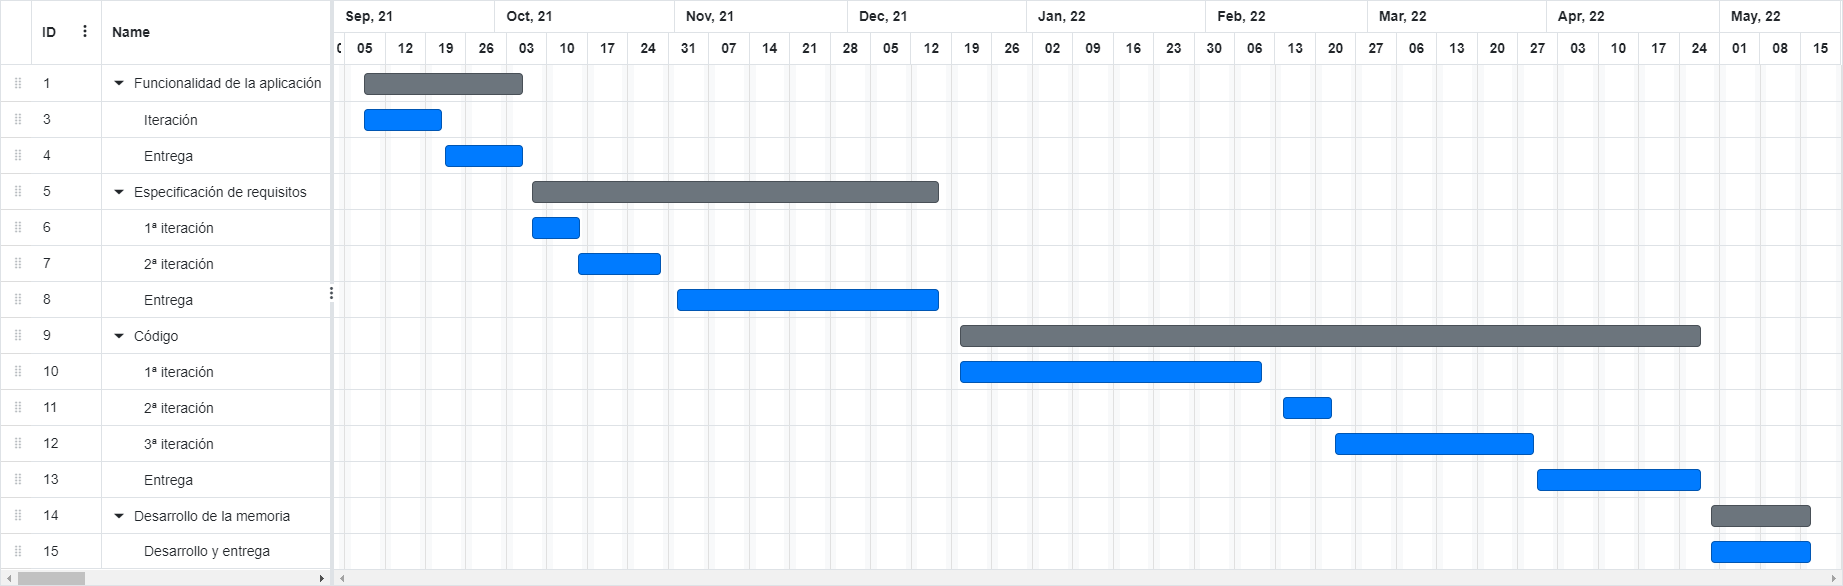
\includegraphics[width=\textwidth]{Images/gantt.png}
    \caption{Gantt chart of project planning}
    \label{fig:gantt}
\end{figure}

During the first phase, the main functionalities of the application were established. Once this phase was completed, the requirements were specified as well as the actors and modules that make up the application. Two iterations were carried out in order to establish the final requirements.

Subsequently, three code iterations were established, in each of which the different modules previously established (login, diet, current diet) were developed. After the code iterations, different white box tests were performed on the different use cases. In the last phase, the memory that complements the code was developed.

In order to carry out the different phases mentioned above, the team held meetings every Saturday, in order to establish the functionality to be developed during the week. At the same time, the meetings helped to know what the team members had done during the previous week, as well as to try to solve together the problems that arose.
\parindent=0em
% El comando "\chp" es como el "\chapter" pero mete "Chapter" en vez de "Capitulo"
\chp{1}{Introduction}

% addtocounter: necesario para tener el mismo número de \section que el de español ==> -2 porque hay 2 secciones en el capitulo 9
\addtocounter{section}{-4}

\pagenumbering{arabic}
\noindent
% \texttt{Lorem ipsum dolor sit amet, consectetuer ad}\\
This chapter will explain the motivation, objectives, work structure and work planning for this project.

\section{Motivation}
% When a person decides to perform any activity with the aim of improving their physical condition, either by increasing or decreasing their weight, they realize that one of the most important factors in achieving this goal is the planning of a healthy and balanced diet.

% For this purpose, complementary tools can be used to carry out this planning, to follow a balanced diet and to plan the different meals during the day.

% With the aim of helping all these users, it has been decided to develop an Android application, in which users will be allowed to follow other diets created. Using this application, the user's eating habits can be improved, keeping a count of calories consumed, understanding food labeling, consulting the nutritional information of the food or even elaborating diets to help the rest of the users.

% introducir el dominio
Every athlete needs to accompany his or her activity with an adequate diet, since nutrition is one of the factors on which physical performance depends. An adequate diet provides the necessary nutrients to maintain an optimal state of health, which translates into performance. Depending on how an athlete eats, you can see how food affects their performance, improving performance and recovery, limiting or even decreasing them, as poor nutrition can promote injuries and fatigue.

% plantear el problema
Currently, there are no mobile applications that can flexibly manage the diets that an athlete needs to follow in order to have a healthy diet that is appropriate to his or her profile. In addition, most of the existing diets on the Internet lack sources or studies that support them and do not have reliable feedback from users who have tried them.

% propuesta que planteamos
To solve these limitations, it has been decided to create an Android application that meets the needs of monitoring and control of diets. It is also possible to see the feedback of the athletes who have followed and evaluated the diet, playing the role of a social network and helping other athletes who are looking for similar goals. In addition, athletes can attach documents to the diets to provide additional information to support them.
\section{Objectives}
The main objective of this project is to develop an Android application that helps athletes to complement their physical activity, following a healthy and balanced diet to achieve the desired physical shape. It is also possible to interact with other athletes, creating diets that can be followed by other athletes or including comments and evaluations in them.

More specific objectives can be defined based on the main objective:
\begin{itemize}
    \item Allow an athlete to register in the application to discover and analyze all the diets in the application, and to update the weight and insert the daily steps, in order to keep a tally and visualize the progress in graphs.
    \item Allow athletes to follow a diet inserted from the application by any of the users, whether they are athletes or administrators.
    \item To offer the possibility to the athlete to evaluate the diet he/she is following, in order to help other athletes to decide and know which diets are being effective.
    \item Allow all athletes the ability to create one or more diets, detailing the foods that compose it, the recommended amount of each one of them and even publishing documentation that helps to follow the diet.
    \item Allow athletes to add foods to diets and have their nutritional information updated at all times.
\end{itemize}
\section{Organización de la memoria}
A continuación se describe de manera breve la estructura de la memoria:

\begin{itemize}
    \item \textbf{Capítulo 1:} en este capítulo se describe la motivación del trabajo, los objetivos y la estructura de la memoria.
    \item \textbf{Capítulo 2:} en este capítulo se estudian herramientas similares a la que se ha realizado en el trabajo.
    \item \textbf{Capítulo 3:} en este capítulo se describe la tecnología utilizada para implementar el proyecto.
    \item \textbf{Capítulo 4:} en este capítulo se definen los actores y casos de uso que se explicarán mediante tablas junto a sus requisitos.
    \item \textbf{Capítulo 5:} en este capítulo se explica el diagrama entidad relación en el que se ha basado el proyecto y la implementación de la base de datos.
    \item \textbf{Capítulo 6:} en este capítulo se explica la arquitectura de la aplicación y los patrones utilizados.
    \item \textbf{Capítulo 7:} en este capítulo se realiza un estudio sobre el diseño e implementación de los casos de uso más relevantes.
    \item \textbf{Capítulo 8:} en este capítulo se exponen las estadísticas aportadas por usuarios que han dado su opinión sobre el producto.
    \item \textbf{Capítulo 9:} en este capítulo se enumeran los casos de uso que se harán en un futuro explicándolos brevemente.
    \item \textbf{Capítulo 10:} en este capítulo se expone el trabajo realizado por cada uno de los autores.
    \item \textbf{Anexo I:} manual de usuario.
    \item \textbf{Anexo II:} preguntas de evaluación.

\end{itemize}

\section{Planning}
This part describes all the planning carried out during the development of this project, detailing the different meetings and iterations performed. In figure  \ref{fig:gantt} the following \textbf{\textit{Gantt}} diagram can be seen where the different phases of the project are indicated.
\begin{figure}[H]
    \centering
    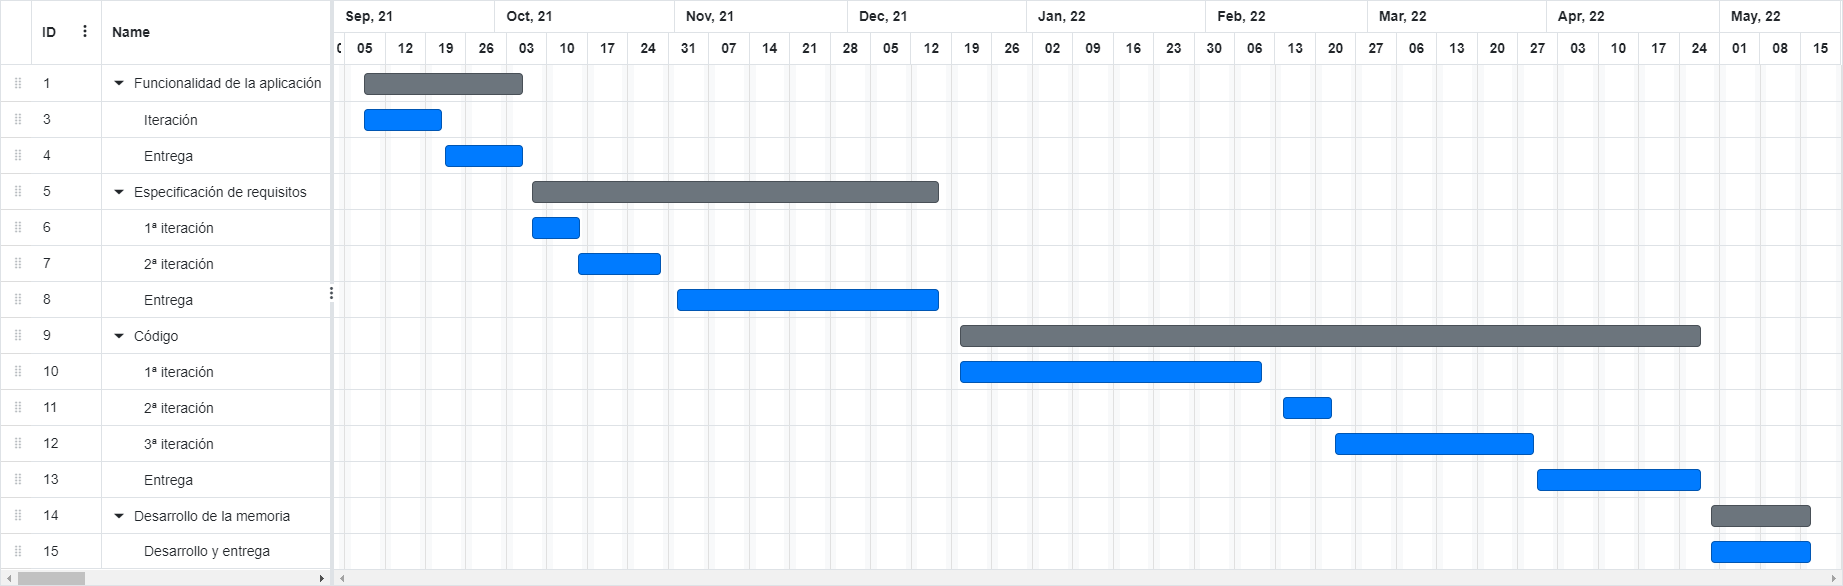
\includegraphics[width=\textwidth]{Images/gantt.png}
    \caption{Gantt chart of project planning}
    \label{fig:gantt}
\end{figure}

During the first phase, the main functionalities of the application were established. Once this phase was completed, the requirements were specified as well as the actors and modules that make up the application. Two iterations were carried out in order to establish the final requirements.

Subsequently, three code iterations were established, in each of which the different modules previously established (login, diet, current diet) were developed. After the code iterations, different white box tests were performed on the different use cases. In the last phase, the memory that complements the code was developed.

In order to carry out the different phases mentioned above, the team held meetings every Saturday, in order to establish the functionality to be developed during the week. At the same time, the meetings helped to know what the team members had done during the previous week, as well as to try to solve together the problems that arose.
\parindent=0em
% El comando "\chp" es como el "\chapter" pero mete "Chapter" en vez de "Capitulo"
\chp{1}{Introduction}

% addtocounter: necesario para tener el mismo número de \section que el de español ==> -2 porque hay 2 secciones en el capitulo 9
\addtocounter{section}{-4}

\pagenumbering{arabic}
\noindent
% \texttt{Lorem ipsum dolor sit amet, consectetuer ad}\\
This chapter will explain the motivation, objectives, work structure and work planning for this project.

\section{Motivation}
% When a person decides to perform any activity with the aim of improving their physical condition, either by increasing or decreasing their weight, they realize that one of the most important factors in achieving this goal is the planning of a healthy and balanced diet.

% For this purpose, complementary tools can be used to carry out this planning, to follow a balanced diet and to plan the different meals during the day.

% With the aim of helping all these users, it has been decided to develop an Android application, in which users will be allowed to follow other diets created. Using this application, the user's eating habits can be improved, keeping a count of calories consumed, understanding food labeling, consulting the nutritional information of the food or even elaborating diets to help the rest of the users.

% introducir el dominio
Every athlete needs to accompany his or her activity with an adequate diet, since nutrition is one of the factors on which physical performance depends. An adequate diet provides the necessary nutrients to maintain an optimal state of health, which translates into performance. Depending on how an athlete eats, you can see how food affects their performance, improving performance and recovery, limiting or even decreasing them, as poor nutrition can promote injuries and fatigue.

% plantear el problema
Currently, there are no mobile applications that can flexibly manage the diets that an athlete needs to follow in order to have a healthy diet that is appropriate to his or her profile. In addition, most of the existing diets on the Internet lack sources or studies that support them and do not have reliable feedback from users who have tried them.

% propuesta que planteamos
To solve these limitations, it has been decided to create an Android application that meets the needs of monitoring and control of diets. It is also possible to see the feedback of the athletes who have followed and evaluated the diet, playing the role of a social network and helping other athletes who are looking for similar goals. In addition, athletes can attach documents to the diets to provide additional information to support them.
\section{Objectives}
The main objective of this project is to develop an Android application that helps athletes to complement their physical activity, following a healthy and balanced diet to achieve the desired physical shape. It is also possible to interact with other athletes, creating diets that can be followed by other athletes or including comments and evaluations in them.

More specific objectives can be defined based on the main objective:
\begin{itemize}
    \item Allow an athlete to register in the application to discover and analyze all the diets in the application, and to update the weight and insert the daily steps, in order to keep a tally and visualize the progress in graphs.
    \item Allow athletes to follow a diet inserted from the application by any of the users, whether they are athletes or administrators.
    \item To offer the possibility to the athlete to evaluate the diet he/she is following, in order to help other athletes to decide and know which diets are being effective.
    \item Allow all athletes the ability to create one or more diets, detailing the foods that compose it, the recommended amount of each one of them and even publishing documentation that helps to follow the diet.
    \item Allow athletes to add foods to diets and have their nutritional information updated at all times.
\end{itemize}
\section{Organización de la memoria}
A continuación se describe de manera breve la estructura de la memoria:

\begin{itemize}
    \item \textbf{Capítulo 1:} en este capítulo se describe la motivación del trabajo, los objetivos y la estructura de la memoria.
    \item \textbf{Capítulo 2:} en este capítulo se estudian herramientas similares a la que se ha realizado en el trabajo.
    \item \textbf{Capítulo 3:} en este capítulo se describe la tecnología utilizada para implementar el proyecto.
    \item \textbf{Capítulo 4:} en este capítulo se definen los actores y casos de uso que se explicarán mediante tablas junto a sus requisitos.
    \item \textbf{Capítulo 5:} en este capítulo se explica el diagrama entidad relación en el que se ha basado el proyecto y la implementación de la base de datos.
    \item \textbf{Capítulo 6:} en este capítulo se explica la arquitectura de la aplicación y los patrones utilizados.
    \item \textbf{Capítulo 7:} en este capítulo se realiza un estudio sobre el diseño e implementación de los casos de uso más relevantes.
    \item \textbf{Capítulo 8:} en este capítulo se exponen las estadísticas aportadas por usuarios que han dado su opinión sobre el producto.
    \item \textbf{Capítulo 9:} en este capítulo se enumeran los casos de uso que se harán en un futuro explicándolos brevemente.
    \item \textbf{Capítulo 10:} en este capítulo se expone el trabajo realizado por cada uno de los autores.
    \item \textbf{Anexo I:} manual de usuario.
    \item \textbf{Anexo II:} preguntas de evaluación.

\end{itemize}

\section{Planning}
This part describes all the planning carried out during the development of this project, detailing the different meetings and iterations performed. In figure  \ref{fig:gantt} the following \textbf{\textit{Gantt}} diagram can be seen where the different phases of the project are indicated.
\begin{figure}[H]
    \centering
    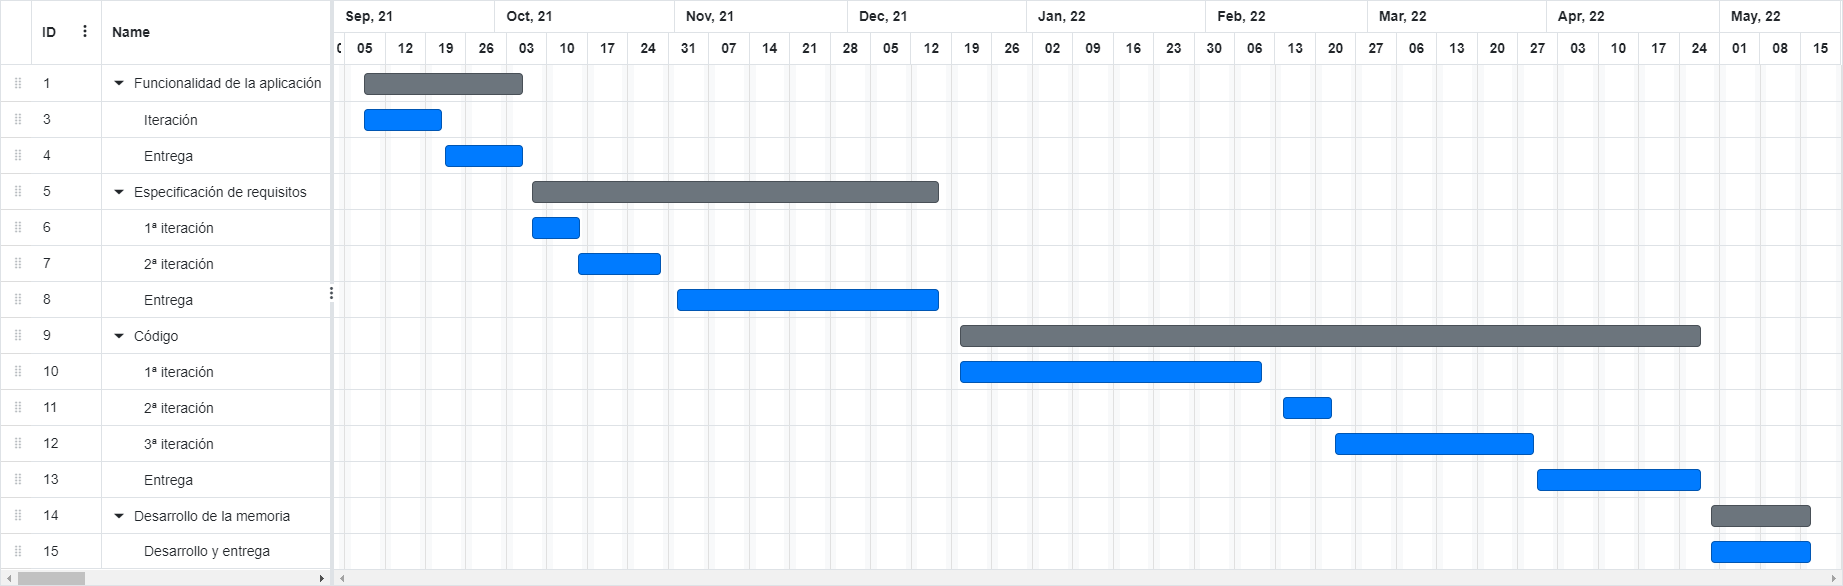
\includegraphics[width=\textwidth]{Images/gantt.png}
    \caption{Gantt chart of project planning}
    \label{fig:gantt}
\end{figure}

During the first phase, the main functionalities of the application were established. Once this phase was completed, the requirements were specified as well as the actors and modules that make up the application. Two iterations were carried out in order to establish the final requirements.

Subsequently, three code iterations were established, in each of which the different modules previously established (login, diet, current diet) were developed. After the code iterations, different white box tests were performed on the different use cases. In the last phase, the memory that complements the code was developed.

In order to carry out the different phases mentioned above, the team held meetings every Saturday, in order to establish the functionality to be developed during the week. At the same time, the meetings helped to know what the team members had done during the previous week, as well as to try to solve together the problems that arose.
\parindent=0em
% El comando "\chp" es como el "\chapter" pero mete "Chapter" en vez de "Capitulo"
\chp{1}{Introduction}

% addtocounter: necesario para tener el mismo número de \section que el de español ==> -2 porque hay 2 secciones en el capitulo 9
\addtocounter{section}{-4}

\pagenumbering{arabic}
\noindent
% \texttt{Lorem ipsum dolor sit amet, consectetuer ad}\\
This chapter will explain the motivation, objectives, work structure and work planning for this project.

\section{Motivation}
% When a person decides to perform any activity with the aim of improving their physical condition, either by increasing or decreasing their weight, they realize that one of the most important factors in achieving this goal is the planning of a healthy and balanced diet.

% For this purpose, complementary tools can be used to carry out this planning, to follow a balanced diet and to plan the different meals during the day.

% With the aim of helping all these users, it has been decided to develop an Android application, in which users will be allowed to follow other diets created. Using this application, the user's eating habits can be improved, keeping a count of calories consumed, understanding food labeling, consulting the nutritional information of the food or even elaborating diets to help the rest of the users.

% introducir el dominio
Every athlete needs to accompany his or her activity with an adequate diet, since nutrition is one of the factors on which physical performance depends. An adequate diet provides the necessary nutrients to maintain an optimal state of health, which translates into performance. Depending on how an athlete eats, you can see how food affects their performance, improving performance and recovery, limiting or even decreasing them, as poor nutrition can promote injuries and fatigue.

% plantear el problema
Currently, there are no mobile applications that can flexibly manage the diets that an athlete needs to follow in order to have a healthy diet that is appropriate to his or her profile. In addition, most of the existing diets on the Internet lack sources or studies that support them and do not have reliable feedback from users who have tried them.

% propuesta que planteamos
To solve these limitations, it has been decided to create an Android application that meets the needs of monitoring and control of diets. It is also possible to see the feedback of the athletes who have followed and evaluated the diet, playing the role of a social network and helping other athletes who are looking for similar goals. In addition, athletes can attach documents to the diets to provide additional information to support them.
\section{Objectives}
The main objective of this project is to develop an Android application that helps athletes to complement their physical activity, following a healthy and balanced diet to achieve the desired physical shape. It is also possible to interact with other athletes, creating diets that can be followed by other athletes or including comments and evaluations in them.

More specific objectives can be defined based on the main objective:
\begin{itemize}
    \item Allow an athlete to register in the application to discover and analyze all the diets in the application, and to update the weight and insert the daily steps, in order to keep a tally and visualize the progress in graphs.
    \item Allow athletes to follow a diet inserted from the application by any of the users, whether they are athletes or administrators.
    \item To offer the possibility to the athlete to evaluate the diet he/she is following, in order to help other athletes to decide and know which diets are being effective.
    \item Allow all athletes the ability to create one or more diets, detailing the foods that compose it, the recommended amount of each one of them and even publishing documentation that helps to follow the diet.
    \item Allow athletes to add foods to diets and have their nutritional information updated at all times.
\end{itemize}
\section{Organización de la memoria}
A continuación se describe de manera breve la estructura de la memoria:

\begin{itemize}
    \item \textbf{Capítulo 1:} en este capítulo se describe la motivación del trabajo, los objetivos y la estructura de la memoria.
    \item \textbf{Capítulo 2:} en este capítulo se estudian herramientas similares a la que se ha realizado en el trabajo.
    \item \textbf{Capítulo 3:} en este capítulo se describe la tecnología utilizada para implementar el proyecto.
    \item \textbf{Capítulo 4:} en este capítulo se definen los actores y casos de uso que se explicarán mediante tablas junto a sus requisitos.
    \item \textbf{Capítulo 5:} en este capítulo se explica el diagrama entidad relación en el que se ha basado el proyecto y la implementación de la base de datos.
    \item \textbf{Capítulo 6:} en este capítulo se explica la arquitectura de la aplicación y los patrones utilizados.
    \item \textbf{Capítulo 7:} en este capítulo se realiza un estudio sobre el diseño e implementación de los casos de uso más relevantes.
    \item \textbf{Capítulo 8:} en este capítulo se exponen las estadísticas aportadas por usuarios que han dado su opinión sobre el producto.
    \item \textbf{Capítulo 9:} en este capítulo se enumeran los casos de uso que se harán en un futuro explicándolos brevemente.
    \item \textbf{Capítulo 10:} en este capítulo se expone el trabajo realizado por cada uno de los autores.
    \item \textbf{Anexo I:} manual de usuario.
    \item \textbf{Anexo II:} preguntas de evaluación.

\end{itemize}

\section{Planning}
This part describes all the planning carried out during the development of this project, detailing the different meetings and iterations performed. In figure  \ref{fig:gantt} the following \textbf{\textit{Gantt}} diagram can be seen where the different phases of the project are indicated.
\begin{figure}[H]
    \centering
    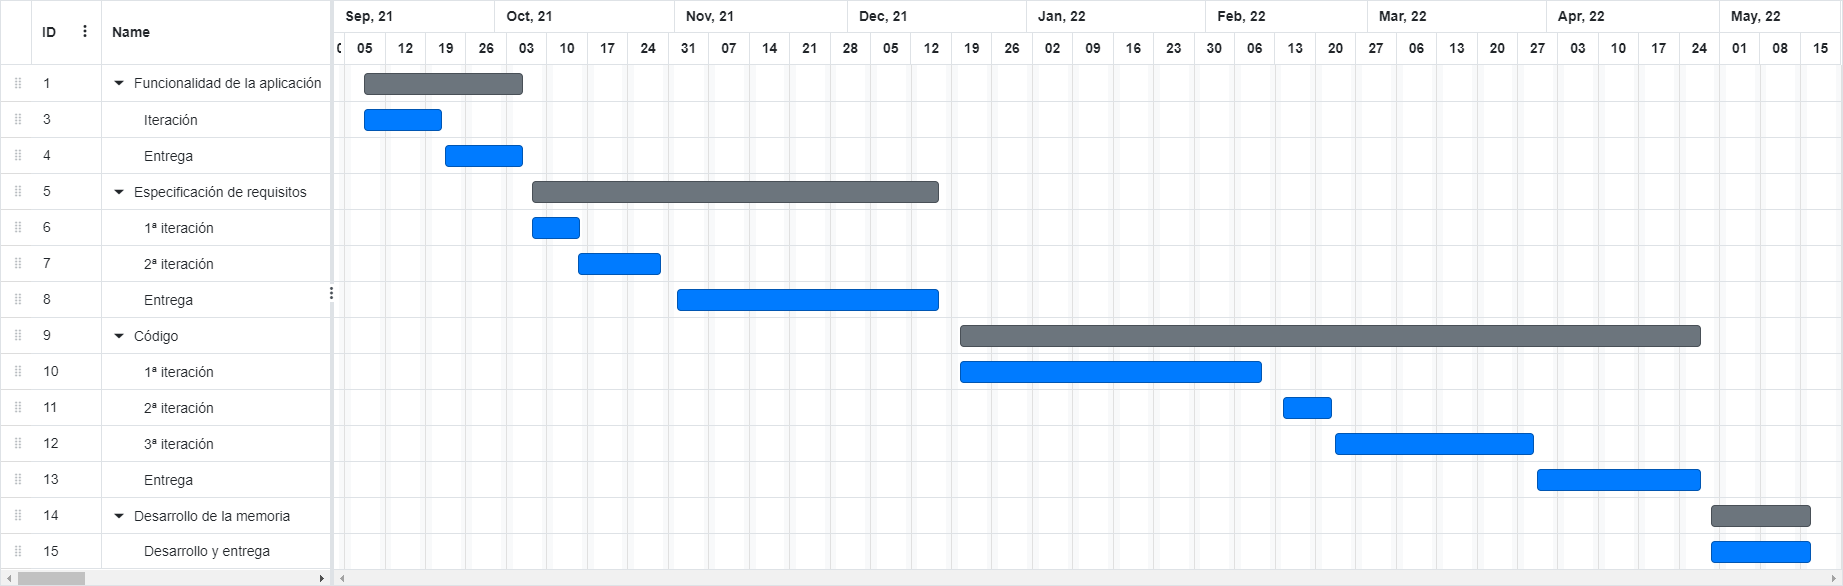
\includegraphics[width=\textwidth]{Images/gantt.png}
    \caption{Gantt chart of project planning}
    \label{fig:gantt}
\end{figure}

During the first phase, the main functionalities of the application were established. Once this phase was completed, the requirements were specified as well as the actors and modules that make up the application. Two iterations were carried out in order to establish the final requirements.

Subsequently, three code iterations were established, in each of which the different modules previously established (login, diet, current diet) were developed. After the code iterations, different white box tests were performed on the different use cases. In the last phase, the memory that complements the code was developed.

In order to carry out the different phases mentioned above, the team held meetings every Saturday, in order to establish the functionality to be developed during the week. At the same time, the meetings helped to know what the team members had done during the previous week, as well as to try to solve together the problems that arose.
\parindent=0em
% El comando "\chp" es como el "\chapter" pero mete "Chapter" en vez de "Capitulo"
\chp{1}{Introduction}

% addtocounter: necesario para tener el mismo número de \section que el de español ==> -2 porque hay 2 secciones en el capitulo 9
\addtocounter{section}{-4}

\pagenumbering{arabic}
\noindent
% \texttt{Lorem ipsum dolor sit amet, consectetuer ad}\\
This chapter will explain the motivation, objectives, work structure and work planning for this project.

\section{Motivation}
% When a person decides to perform any activity with the aim of improving their physical condition, either by increasing or decreasing their weight, they realize that one of the most important factors in achieving this goal is the planning of a healthy and balanced diet.

% For this purpose, complementary tools can be used to carry out this planning, to follow a balanced diet and to plan the different meals during the day.

% With the aim of helping all these users, it has been decided to develop an Android application, in which users will be allowed to follow other diets created. Using this application, the user's eating habits can be improved, keeping a count of calories consumed, understanding food labeling, consulting the nutritional information of the food or even elaborating diets to help the rest of the users.

% introducir el dominio
Every athlete needs to accompany his or her activity with an adequate diet, since nutrition is one of the factors on which physical performance depends. An adequate diet provides the necessary nutrients to maintain an optimal state of health, which translates into performance. Depending on how an athlete eats, you can see how food affects their performance, improving performance and recovery, limiting or even decreasing them, as poor nutrition can promote injuries and fatigue.

% plantear el problema
Currently, there are no mobile applications that can flexibly manage the diets that an athlete needs to follow in order to have a healthy diet that is appropriate to his or her profile. In addition, most of the existing diets on the Internet lack sources or studies that support them and do not have reliable feedback from users who have tried them.

% propuesta que planteamos
To solve these limitations, it has been decided to create an Android application that meets the needs of monitoring and control of diets. It is also possible to see the feedback of the athletes who have followed and evaluated the diet, playing the role of a social network and helping other athletes who are looking for similar goals. In addition, athletes can attach documents to the diets to provide additional information to support them.
\section{Objectives}
The main objective of this project is to develop an Android application that helps athletes to complement their physical activity, following a healthy and balanced diet to achieve the desired physical shape. It is also possible to interact with other athletes, creating diets that can be followed by other athletes or including comments and evaluations in them.

More specific objectives can be defined based on the main objective:
\begin{itemize}
    \item Allow an athlete to register in the application to discover and analyze all the diets in the application, and to update the weight and insert the daily steps, in order to keep a tally and visualize the progress in graphs.
    \item Allow athletes to follow a diet inserted from the application by any of the users, whether they are athletes or administrators.
    \item To offer the possibility to the athlete to evaluate the diet he/she is following, in order to help other athletes to decide and know which diets are being effective.
    \item Allow all athletes the ability to create one or more diets, detailing the foods that compose it, the recommended amount of each one of them and even publishing documentation that helps to follow the diet.
    \item Allow athletes to add foods to diets and have their nutritional information updated at all times.
\end{itemize}
\section{Organización de la memoria}
A continuación se describe de manera breve la estructura de la memoria:

\begin{itemize}
    \item \textbf{Capítulo 1:} en este capítulo se describe la motivación del trabajo, los objetivos y la estructura de la memoria.
    \item \textbf{Capítulo 2:} en este capítulo se estudian herramientas similares a la que se ha realizado en el trabajo.
    \item \textbf{Capítulo 3:} en este capítulo se describe la tecnología utilizada para implementar el proyecto.
    \item \textbf{Capítulo 4:} en este capítulo se definen los actores y casos de uso que se explicarán mediante tablas junto a sus requisitos.
    \item \textbf{Capítulo 5:} en este capítulo se explica el diagrama entidad relación en el que se ha basado el proyecto y la implementación de la base de datos.
    \item \textbf{Capítulo 6:} en este capítulo se explica la arquitectura de la aplicación y los patrones utilizados.
    \item \textbf{Capítulo 7:} en este capítulo se realiza un estudio sobre el diseño e implementación de los casos de uso más relevantes.
    \item \textbf{Capítulo 8:} en este capítulo se exponen las estadísticas aportadas por usuarios que han dado su opinión sobre el producto.
    \item \textbf{Capítulo 9:} en este capítulo se enumeran los casos de uso que se harán en un futuro explicándolos brevemente.
    \item \textbf{Capítulo 10:} en este capítulo se expone el trabajo realizado por cada uno de los autores.
    \item \textbf{Anexo I:} manual de usuario.
    \item \textbf{Anexo II:} preguntas de evaluación.

\end{itemize}

\section{Planning}
This part describes all the planning carried out during the development of this project, detailing the different meetings and iterations performed. In figure  \ref{fig:gantt} the following \textbf{\textit{Gantt}} diagram can be seen where the different phases of the project are indicated.
\begin{figure}[H]
    \centering
    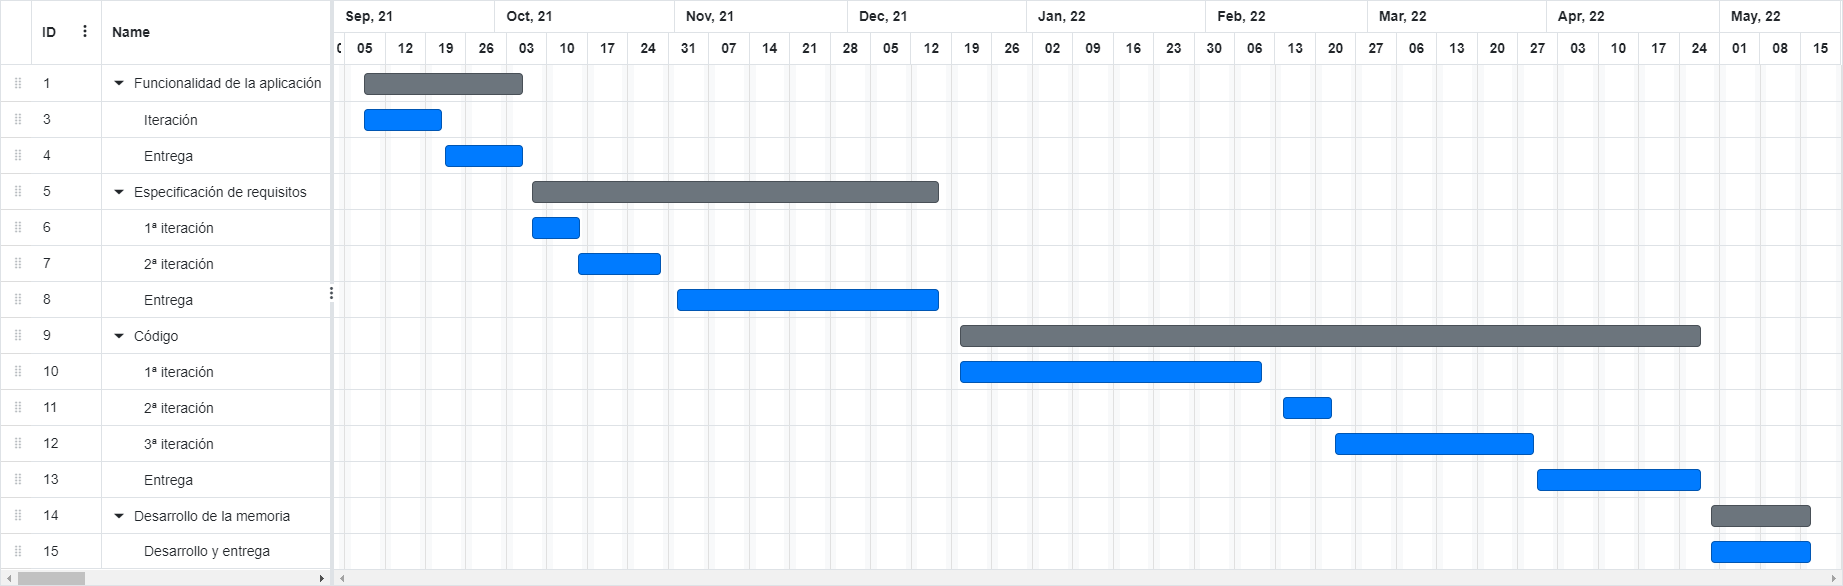
\includegraphics[width=\textwidth]{Images/gantt.png}
    \caption{Gantt chart of project planning}
    \label{fig:gantt}
\end{figure}

During the first phase, the main functionalities of the application were established. Once this phase was completed, the requirements were specified as well as the actors and modules that make up the application. Two iterations were carried out in order to establish the final requirements.

Subsequently, three code iterations were established, in each of which the different modules previously established (login, diet, current diet) were developed. After the code iterations, different white box tests were performed on the different use cases. In the last phase, the memory that complements the code was developed.

In order to carry out the different phases mentioned above, the team held meetings every Saturday, in order to establish the functionality to be developed during the week. At the same time, the meetings helped to know what the team members had done during the previous week, as well as to try to solve together the problems that arose.
\parindent=0em
% El comando "\chp" es como el "\chapter" pero mete "Chapter" en vez de "Capitulo"
\chp{1}{Introduction}

% addtocounter: necesario para tener el mismo número de \section que el de español ==> -2 porque hay 2 secciones en el capitulo 9
\addtocounter{section}{-4}

\pagenumbering{arabic}
\noindent
% \texttt{Lorem ipsum dolor sit amet, consectetuer ad}\\
This chapter will explain the motivation, objectives, work structure and work planning for this project.

\section{Motivation}
% When a person decides to perform any activity with the aim of improving their physical condition, either by increasing or decreasing their weight, they realize that one of the most important factors in achieving this goal is the planning of a healthy and balanced diet.

% For this purpose, complementary tools can be used to carry out this planning, to follow a balanced diet and to plan the different meals during the day.

% With the aim of helping all these users, it has been decided to develop an Android application, in which users will be allowed to follow other diets created. Using this application, the user's eating habits can be improved, keeping a count of calories consumed, understanding food labeling, consulting the nutritional information of the food or even elaborating diets to help the rest of the users.

% introducir el dominio
Every athlete needs to accompany his or her activity with an adequate diet, since nutrition is one of the factors on which physical performance depends. An adequate diet provides the necessary nutrients to maintain an optimal state of health, which translates into performance. Depending on how an athlete eats, you can see how food affects their performance, improving performance and recovery, limiting or even decreasing them, as poor nutrition can promote injuries and fatigue.

% plantear el problema
Currently, there are no mobile applications that can flexibly manage the diets that an athlete needs to follow in order to have a healthy diet that is appropriate to his or her profile. In addition, most of the existing diets on the Internet lack sources or studies that support them and do not have reliable feedback from users who have tried them.

% propuesta que planteamos
To solve these limitations, it has been decided to create an Android application that meets the needs of monitoring and control of diets. It is also possible to see the feedback of the athletes who have followed and evaluated the diet, playing the role of a social network and helping other athletes who are looking for similar goals. In addition, athletes can attach documents to the diets to provide additional information to support them.
\section{Objectives}
The main objective of this project is to develop an Android application that helps athletes to complement their physical activity, following a healthy and balanced diet to achieve the desired physical shape. It is also possible to interact with other athletes, creating diets that can be followed by other athletes or including comments and evaluations in them.

More specific objectives can be defined based on the main objective:
\begin{itemize}
    \item Allow an athlete to register in the application to discover and analyze all the diets in the application, and to update the weight and insert the daily steps, in order to keep a tally and visualize the progress in graphs.
    \item Allow athletes to follow a diet inserted from the application by any of the users, whether they are athletes or administrators.
    \item To offer the possibility to the athlete to evaluate the diet he/she is following, in order to help other athletes to decide and know which diets are being effective.
    \item Allow all athletes the ability to create one or more diets, detailing the foods that compose it, the recommended amount of each one of them and even publishing documentation that helps to follow the diet.
    \item Allow athletes to add foods to diets and have their nutritional information updated at all times.
\end{itemize}
\section{Organización de la memoria}
A continuación se describe de manera breve la estructura de la memoria:

\begin{itemize}
    \item \textbf{Capítulo 1:} en este capítulo se describe la motivación del trabajo, los objetivos y la estructura de la memoria.
    \item \textbf{Capítulo 2:} en este capítulo se estudian herramientas similares a la que se ha realizado en el trabajo.
    \item \textbf{Capítulo 3:} en este capítulo se describe la tecnología utilizada para implementar el proyecto.
    \item \textbf{Capítulo 4:} en este capítulo se definen los actores y casos de uso que se explicarán mediante tablas junto a sus requisitos.
    \item \textbf{Capítulo 5:} en este capítulo se explica el diagrama entidad relación en el que se ha basado el proyecto y la implementación de la base de datos.
    \item \textbf{Capítulo 6:} en este capítulo se explica la arquitectura de la aplicación y los patrones utilizados.
    \item \textbf{Capítulo 7:} en este capítulo se realiza un estudio sobre el diseño e implementación de los casos de uso más relevantes.
    \item \textbf{Capítulo 8:} en este capítulo se exponen las estadísticas aportadas por usuarios que han dado su opinión sobre el producto.
    \item \textbf{Capítulo 9:} en este capítulo se enumeran los casos de uso que se harán en un futuro explicándolos brevemente.
    \item \textbf{Capítulo 10:} en este capítulo se expone el trabajo realizado por cada uno de los autores.
    \item \textbf{Anexo I:} manual de usuario.
    \item \textbf{Anexo II:} preguntas de evaluación.

\end{itemize}

\section{Planning}
This part describes all the planning carried out during the development of this project, detailing the different meetings and iterations performed. In figure  \ref{fig:gantt} the following \textbf{\textit{Gantt}} diagram can be seen where the different phases of the project are indicated.
\begin{figure}[H]
    \centering
    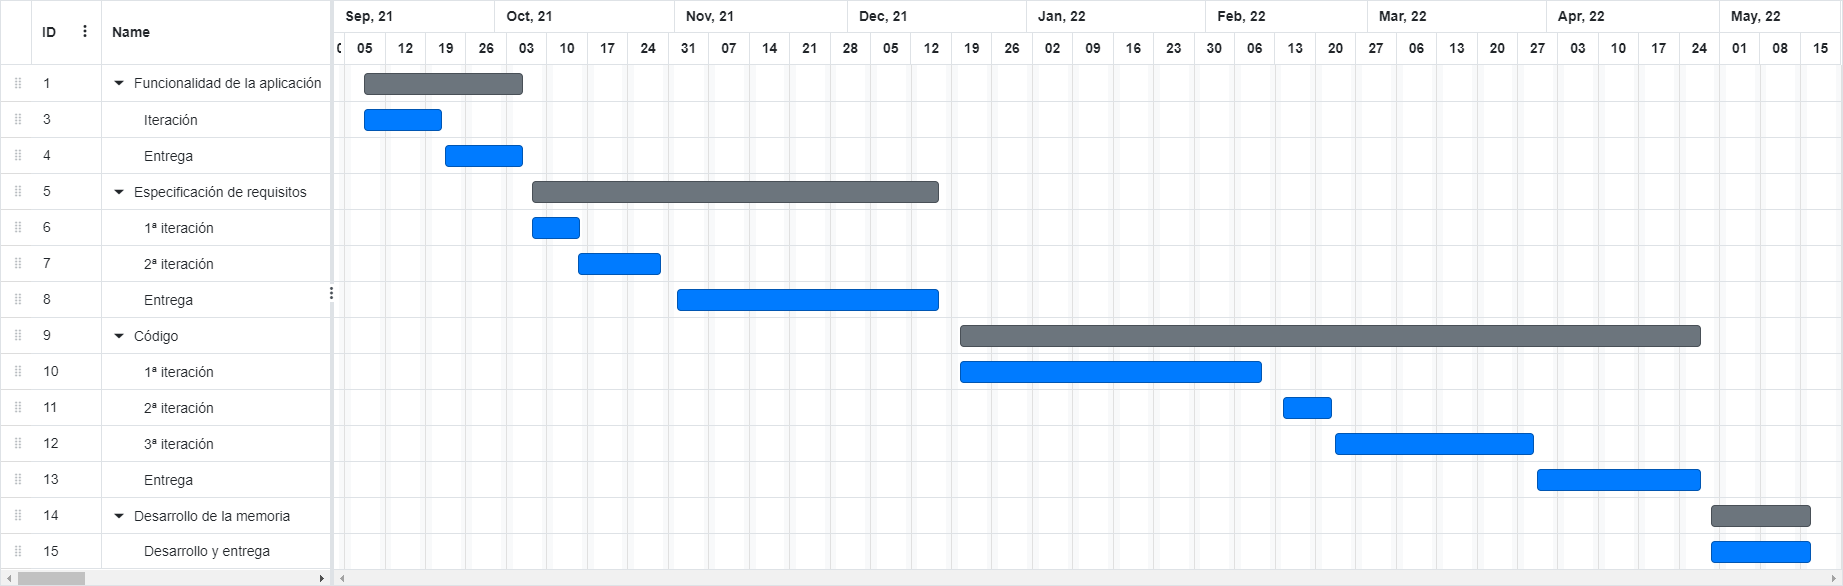
\includegraphics[width=\textwidth]{Images/gantt.png}
    \caption{Gantt chart of project planning}
    \label{fig:gantt}
\end{figure}

During the first phase, the main functionalities of the application were established. Once this phase was completed, the requirements were specified as well as the actors and modules that make up the application. Two iterations were carried out in order to establish the final requirements.

Subsequently, three code iterations were established, in each of which the different modules previously established (login, diet, current diet) were developed. After the code iterations, different white box tests were performed on the different use cases. In the last phase, the memory that complements the code was developed.

In order to carry out the different phases mentioned above, the team held meetings every Saturday, in order to establish the functionality to be developed during the week. At the same time, the meetings helped to know what the team members had done during the previous week, as well as to try to solve together the problems that arose.
\parindent=0em
% El comando "\chp" es como el "\chapter" pero mete "Chapter" en vez de "Capitulo"
\chp{1}{Introduction}

% addtocounter: necesario para tener el mismo número de \section que el de español ==> -2 porque hay 2 secciones en el capitulo 9
\addtocounter{section}{-4}

\pagenumbering{arabic}
\noindent
% \texttt{Lorem ipsum dolor sit amet, consectetuer ad}\\
This chapter will explain the motivation, objectives, work structure and work planning for this project.

\section{Motivation}
% When a person decides to perform any activity with the aim of improving their physical condition, either by increasing or decreasing their weight, they realize that one of the most important factors in achieving this goal is the planning of a healthy and balanced diet.

% For this purpose, complementary tools can be used to carry out this planning, to follow a balanced diet and to plan the different meals during the day.

% With the aim of helping all these users, it has been decided to develop an Android application, in which users will be allowed to follow other diets created. Using this application, the user's eating habits can be improved, keeping a count of calories consumed, understanding food labeling, consulting the nutritional information of the food or even elaborating diets to help the rest of the users.

% introducir el dominio
Every athlete needs to accompany his or her activity with an adequate diet, since nutrition is one of the factors on which physical performance depends. An adequate diet provides the necessary nutrients to maintain an optimal state of health, which translates into performance. Depending on how an athlete eats, you can see how food affects their performance, improving performance and recovery, limiting or even decreasing them, as poor nutrition can promote injuries and fatigue.

% plantear el problema
Currently, there are no mobile applications that can flexibly manage the diets that an athlete needs to follow in order to have a healthy diet that is appropriate to his or her profile. In addition, most of the existing diets on the Internet lack sources or studies that support them and do not have reliable feedback from users who have tried them.

% propuesta que planteamos
To solve these limitations, it has been decided to create an Android application that meets the needs of monitoring and control of diets. It is also possible to see the feedback of the athletes who have followed and evaluated the diet, playing the role of a social network and helping other athletes who are looking for similar goals. In addition, athletes can attach documents to the diets to provide additional information to support them.
\section{Objectives}
The main objective of this project is to develop an Android application that helps athletes to complement their physical activity, following a healthy and balanced diet to achieve the desired physical shape. It is also possible to interact with other athletes, creating diets that can be followed by other athletes or including comments and evaluations in them.

More specific objectives can be defined based on the main objective:
\begin{itemize}
    \item Allow an athlete to register in the application to discover and analyze all the diets in the application, and to update the weight and insert the daily steps, in order to keep a tally and visualize the progress in graphs.
    \item Allow athletes to follow a diet inserted from the application by any of the users, whether they are athletes or administrators.
    \item To offer the possibility to the athlete to evaluate the diet he/she is following, in order to help other athletes to decide and know which diets are being effective.
    \item Allow all athletes the ability to create one or more diets, detailing the foods that compose it, the recommended amount of each one of them and even publishing documentation that helps to follow the diet.
    \item Allow athletes to add foods to diets and have their nutritional information updated at all times.
\end{itemize}
\section{Organización de la memoria}
A continuación se describe de manera breve la estructura de la memoria:

\begin{itemize}
    \item \textbf{Capítulo 1:} en este capítulo se describe la motivación del trabajo, los objetivos y la estructura de la memoria.
    \item \textbf{Capítulo 2:} en este capítulo se estudian herramientas similares a la que se ha realizado en el trabajo.
    \item \textbf{Capítulo 3:} en este capítulo se describe la tecnología utilizada para implementar el proyecto.
    \item \textbf{Capítulo 4:} en este capítulo se definen los actores y casos de uso que se explicarán mediante tablas junto a sus requisitos.
    \item \textbf{Capítulo 5:} en este capítulo se explica el diagrama entidad relación en el que se ha basado el proyecto y la implementación de la base de datos.
    \item \textbf{Capítulo 6:} en este capítulo se explica la arquitectura de la aplicación y los patrones utilizados.
    \item \textbf{Capítulo 7:} en este capítulo se realiza un estudio sobre el diseño e implementación de los casos de uso más relevantes.
    \item \textbf{Capítulo 8:} en este capítulo se exponen las estadísticas aportadas por usuarios que han dado su opinión sobre el producto.
    \item \textbf{Capítulo 9:} en este capítulo se enumeran los casos de uso que se harán en un futuro explicándolos brevemente.
    \item \textbf{Capítulo 10:} en este capítulo se expone el trabajo realizado por cada uno de los autores.
    \item \textbf{Anexo I:} manual de usuario.
    \item \textbf{Anexo II:} preguntas de evaluación.

\end{itemize}

\section{Planning}
This part describes all the planning carried out during the development of this project, detailing the different meetings and iterations performed. In figure  \ref{fig:gantt} the following \textbf{\textit{Gantt}} diagram can be seen where the different phases of the project are indicated.
\begin{figure}[H]
    \centering
    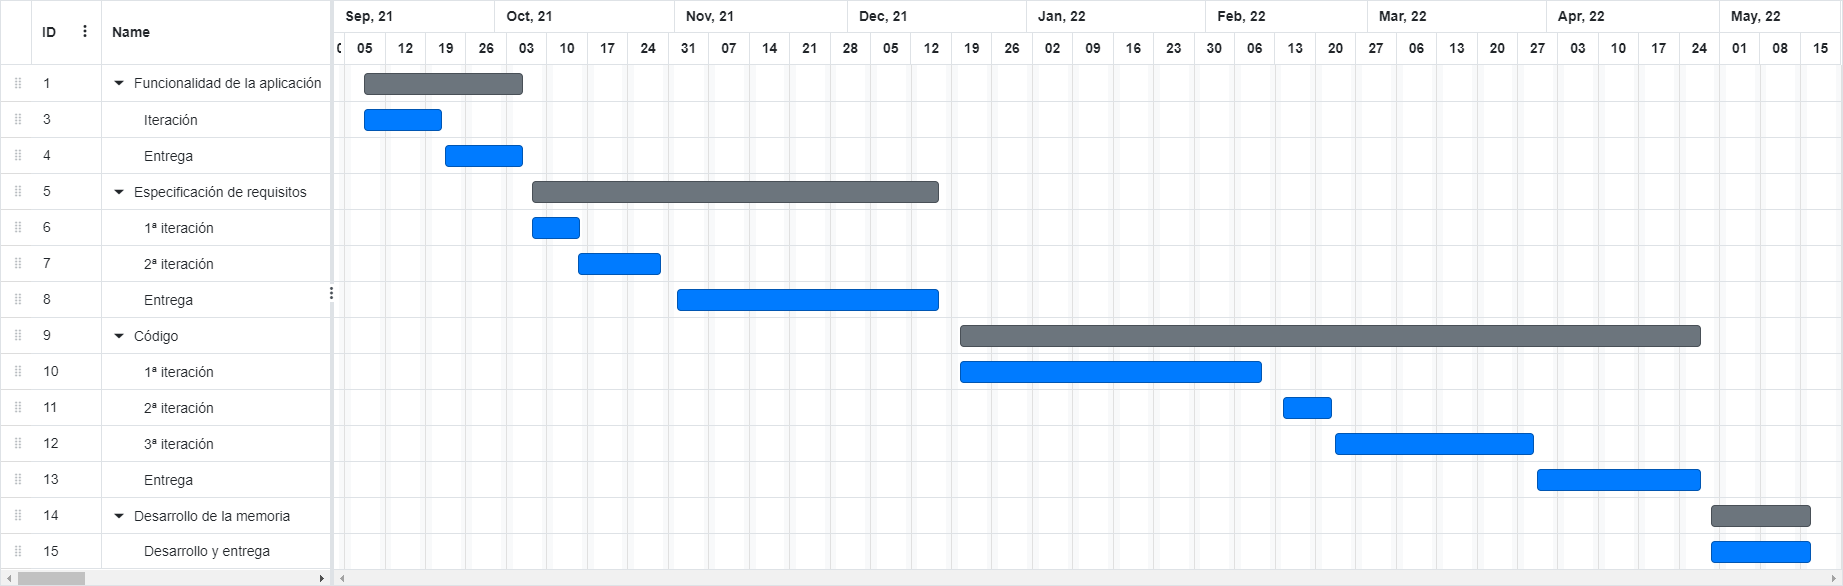
\includegraphics[width=\textwidth]{Images/gantt.png}
    \caption{Gantt chart of project planning}
    \label{fig:gantt}
\end{figure}

During the first phase, the main functionalities of the application were established. Once this phase was completed, the requirements were specified as well as the actors and modules that make up the application. Two iterations were carried out in order to establish the final requirements.

Subsequently, three code iterations were established, in each of which the different modules previously established (login, diet, current diet) were developed. After the code iterations, different white box tests were performed on the different use cases. In the last phase, the memory that complements the code was developed.

In order to carry out the different phases mentioned above, the team held meetings every Saturday, in order to establish the functionality to be developed during the week. At the same time, the meetings helped to know what the team members had done during the previous week, as well as to try to solve together the problems that arose.
\parindent=0em
% El comando "\chp" es como el "\chapter" pero mete "Chapter" en vez de "Capitulo"
\chp{1}{Introduction}

% addtocounter: necesario para tener el mismo número de \section que el de español ==> -2 porque hay 2 secciones en el capitulo 9
\addtocounter{section}{-4}

\pagenumbering{arabic}
\noindent
% \texttt{Lorem ipsum dolor sit amet, consectetuer ad}\\
This chapter will explain the motivation, objectives, work structure and work planning for this project.

\section{Motivation}
% When a person decides to perform any activity with the aim of improving their physical condition, either by increasing or decreasing their weight, they realize that one of the most important factors in achieving this goal is the planning of a healthy and balanced diet.

% For this purpose, complementary tools can be used to carry out this planning, to follow a balanced diet and to plan the different meals during the day.

% With the aim of helping all these users, it has been decided to develop an Android application, in which users will be allowed to follow other diets created. Using this application, the user's eating habits can be improved, keeping a count of calories consumed, understanding food labeling, consulting the nutritional information of the food or even elaborating diets to help the rest of the users.

% introducir el dominio
Every athlete needs to accompany his or her activity with an adequate diet, since nutrition is one of the factors on which physical performance depends. An adequate diet provides the necessary nutrients to maintain an optimal state of health, which translates into performance. Depending on how an athlete eats, you can see how food affects their performance, improving performance and recovery, limiting or even decreasing them, as poor nutrition can promote injuries and fatigue.

% plantear el problema
Currently, there are no mobile applications that can flexibly manage the diets that an athlete needs to follow in order to have a healthy diet that is appropriate to his or her profile. In addition, most of the existing diets on the Internet lack sources or studies that support them and do not have reliable feedback from users who have tried them.

% propuesta que planteamos
To solve these limitations, it has been decided to create an Android application that meets the needs of monitoring and control of diets. It is also possible to see the feedback of the athletes who have followed and evaluated the diet, playing the role of a social network and helping other athletes who are looking for similar goals. In addition, athletes can attach documents to the diets to provide additional information to support them.
\section{Objectives}
The main objective of this project is to develop an Android application that helps athletes to complement their physical activity, following a healthy and balanced diet to achieve the desired physical shape. It is also possible to interact with other athletes, creating diets that can be followed by other athletes or including comments and evaluations in them.

More specific objectives can be defined based on the main objective:
\begin{itemize}
    \item Allow an athlete to register in the application to discover and analyze all the diets in the application, and to update the weight and insert the daily steps, in order to keep a tally and visualize the progress in graphs.
    \item Allow athletes to follow a diet inserted from the application by any of the users, whether they are athletes or administrators.
    \item To offer the possibility to the athlete to evaluate the diet he/she is following, in order to help other athletes to decide and know which diets are being effective.
    \item Allow all athletes the ability to create one or more diets, detailing the foods that compose it, the recommended amount of each one of them and even publishing documentation that helps to follow the diet.
    \item Allow athletes to add foods to diets and have their nutritional information updated at all times.
\end{itemize}
\section{Organización de la memoria}
A continuación se describe de manera breve la estructura de la memoria:

\begin{itemize}
    \item \textbf{Capítulo 1:} en este capítulo se describe la motivación del trabajo, los objetivos y la estructura de la memoria.
    \item \textbf{Capítulo 2:} en este capítulo se estudian herramientas similares a la que se ha realizado en el trabajo.
    \item \textbf{Capítulo 3:} en este capítulo se describe la tecnología utilizada para implementar el proyecto.
    \item \textbf{Capítulo 4:} en este capítulo se definen los actores y casos de uso que se explicarán mediante tablas junto a sus requisitos.
    \item \textbf{Capítulo 5:} en este capítulo se explica el diagrama entidad relación en el que se ha basado el proyecto y la implementación de la base de datos.
    \item \textbf{Capítulo 6:} en este capítulo se explica la arquitectura de la aplicación y los patrones utilizados.
    \item \textbf{Capítulo 7:} en este capítulo se realiza un estudio sobre el diseño e implementación de los casos de uso más relevantes.
    \item \textbf{Capítulo 8:} en este capítulo se exponen las estadísticas aportadas por usuarios que han dado su opinión sobre el producto.
    \item \textbf{Capítulo 9:} en este capítulo se enumeran los casos de uso que se harán en un futuro explicándolos brevemente.
    \item \textbf{Capítulo 10:} en este capítulo se expone el trabajo realizado por cada uno de los autores.
    \item \textbf{Anexo I:} manual de usuario.
    \item \textbf{Anexo II:} preguntas de evaluación.

\end{itemize}

\section{Planning}
This part describes all the planning carried out during the development of this project, detailing the different meetings and iterations performed. In figure  \ref{fig:gantt} the following \textbf{\textit{Gantt}} diagram can be seen where the different phases of the project are indicated.
\begin{figure}[H]
    \centering
    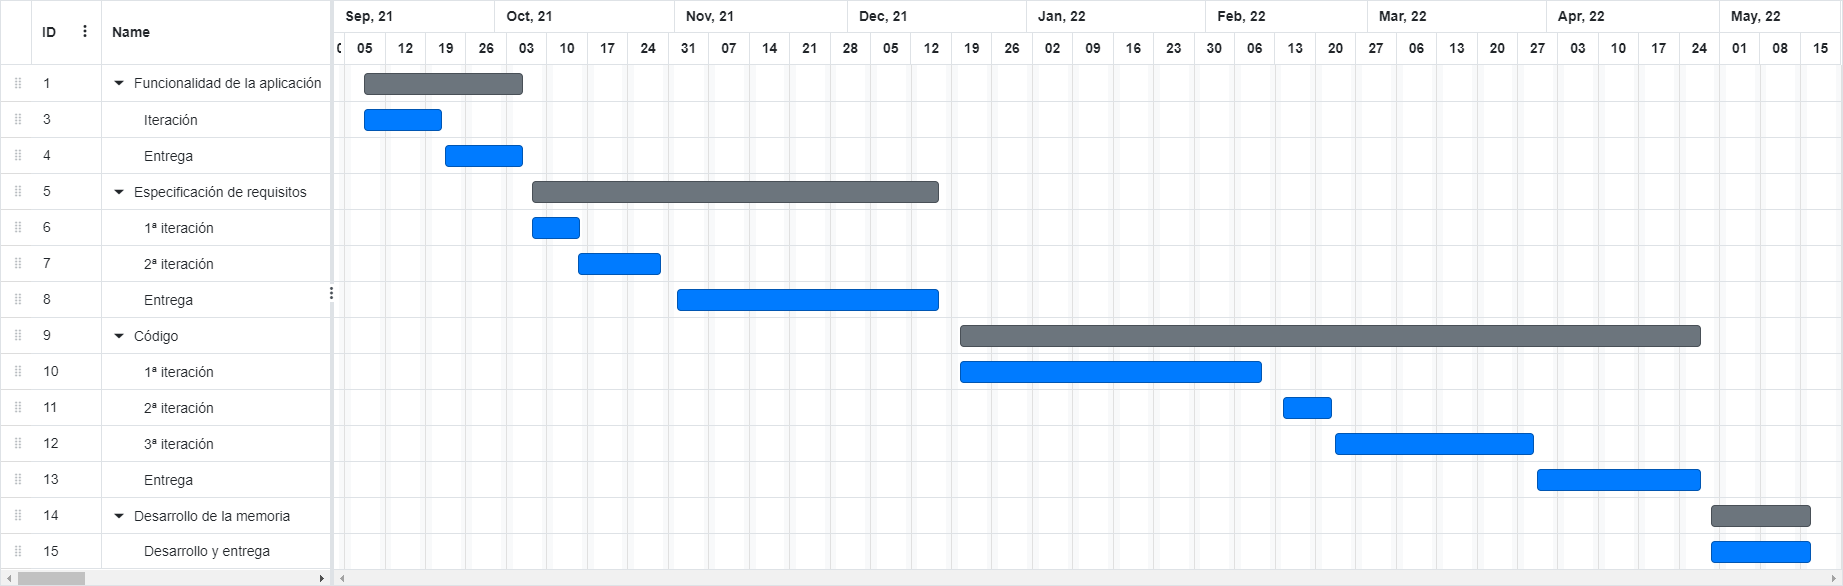
\includegraphics[width=\textwidth]{Images/gantt.png}
    \caption{Gantt chart of project planning}
    \label{fig:gantt}
\end{figure}

During the first phase, the main functionalities of the application were established. Once this phase was completed, the requirements were specified as well as the actors and modules that make up the application. Two iterations were carried out in order to establish the final requirements.

Subsequently, three code iterations were established, in each of which the different modules previously established (login, diet, current diet) were developed. After the code iterations, different white box tests were performed on the different use cases. In the last phase, the memory that complements the code was developed.

In order to carry out the different phases mentioned above, the team held meetings every Saturday, in order to establish the functionality to be developed during the week. At the same time, the meetings helped to know what the team members had done during the previous week, as well as to try to solve together the problems that arose.
\parindent=0em
% El comando "\chp" es como el "\chapter" pero mete "Chapter" en vez de "Capitulo"
\chp{1}{Introduction}

% addtocounter: necesario para tener el mismo número de \section que el de español ==> -2 porque hay 2 secciones en el capitulo 9
\addtocounter{section}{-4}

\pagenumbering{arabic}
\noindent
% \texttt{Lorem ipsum dolor sit amet, consectetuer ad}\\
This chapter will explain the motivation, objectives, work structure and work planning for this project.

\section{Motivation}
% When a person decides to perform any activity with the aim of improving their physical condition, either by increasing or decreasing their weight, they realize that one of the most important factors in achieving this goal is the planning of a healthy and balanced diet.

% For this purpose, complementary tools can be used to carry out this planning, to follow a balanced diet and to plan the different meals during the day.

% With the aim of helping all these users, it has been decided to develop an Android application, in which users will be allowed to follow other diets created. Using this application, the user's eating habits can be improved, keeping a count of calories consumed, understanding food labeling, consulting the nutritional information of the food or even elaborating diets to help the rest of the users.

% introducir el dominio
Every athlete needs to accompany his or her activity with an adequate diet, since nutrition is one of the factors on which physical performance depends. An adequate diet provides the necessary nutrients to maintain an optimal state of health, which translates into performance. Depending on how an athlete eats, you can see how food affects their performance, improving performance and recovery, limiting or even decreasing them, as poor nutrition can promote injuries and fatigue.

% plantear el problema
Currently, there are no mobile applications that can flexibly manage the diets that an athlete needs to follow in order to have a healthy diet that is appropriate to his or her profile. In addition, most of the existing diets on the Internet lack sources or studies that support them and do not have reliable feedback from users who have tried them.

% propuesta que planteamos
To solve these limitations, it has been decided to create an Android application that meets the needs of monitoring and control of diets. It is also possible to see the feedback of the athletes who have followed and evaluated the diet, playing the role of a social network and helping other athletes who are looking for similar goals. In addition, athletes can attach documents to the diets to provide additional information to support them.
\section{Objectives}
The main objective of this project is to develop an Android application that helps athletes to complement their physical activity, following a healthy and balanced diet to achieve the desired physical shape. It is also possible to interact with other athletes, creating diets that can be followed by other athletes or including comments and evaluations in them.

More specific objectives can be defined based on the main objective:
\begin{itemize}
    \item Allow an athlete to register in the application to discover and analyze all the diets in the application, and to update the weight and insert the daily steps, in order to keep a tally and visualize the progress in graphs.
    \item Allow athletes to follow a diet inserted from the application by any of the users, whether they are athletes or administrators.
    \item To offer the possibility to the athlete to evaluate the diet he/she is following, in order to help other athletes to decide and know which diets are being effective.
    \item Allow all athletes the ability to create one or more diets, detailing the foods that compose it, the recommended amount of each one of them and even publishing documentation that helps to follow the diet.
    \item Allow athletes to add foods to diets and have their nutritional information updated at all times.
\end{itemize}
\section{Organización de la memoria}
A continuación se describe de manera breve la estructura de la memoria:

\begin{itemize}
    \item \textbf{Capítulo 1:} en este capítulo se describe la motivación del trabajo, los objetivos y la estructura de la memoria.
    \item \textbf{Capítulo 2:} en este capítulo se estudian herramientas similares a la que se ha realizado en el trabajo.
    \item \textbf{Capítulo 3:} en este capítulo se describe la tecnología utilizada para implementar el proyecto.
    \item \textbf{Capítulo 4:} en este capítulo se definen los actores y casos de uso que se explicarán mediante tablas junto a sus requisitos.
    \item \textbf{Capítulo 5:} en este capítulo se explica el diagrama entidad relación en el que se ha basado el proyecto y la implementación de la base de datos.
    \item \textbf{Capítulo 6:} en este capítulo se explica la arquitectura de la aplicación y los patrones utilizados.
    \item \textbf{Capítulo 7:} en este capítulo se realiza un estudio sobre el diseño e implementación de los casos de uso más relevantes.
    \item \textbf{Capítulo 8:} en este capítulo se exponen las estadísticas aportadas por usuarios que han dado su opinión sobre el producto.
    \item \textbf{Capítulo 9:} en este capítulo se enumeran los casos de uso que se harán en un futuro explicándolos brevemente.
    \item \textbf{Capítulo 10:} en este capítulo se expone el trabajo realizado por cada uno de los autores.
    \item \textbf{Anexo I:} manual de usuario.
    \item \textbf{Anexo II:} preguntas de evaluación.

\end{itemize}

\section{Planning}
This part describes all the planning carried out during the development of this project, detailing the different meetings and iterations performed. In figure  \ref{fig:gantt} the following \textbf{\textit{Gantt}} diagram can be seen where the different phases of the project are indicated.
\begin{figure}[H]
    \centering
    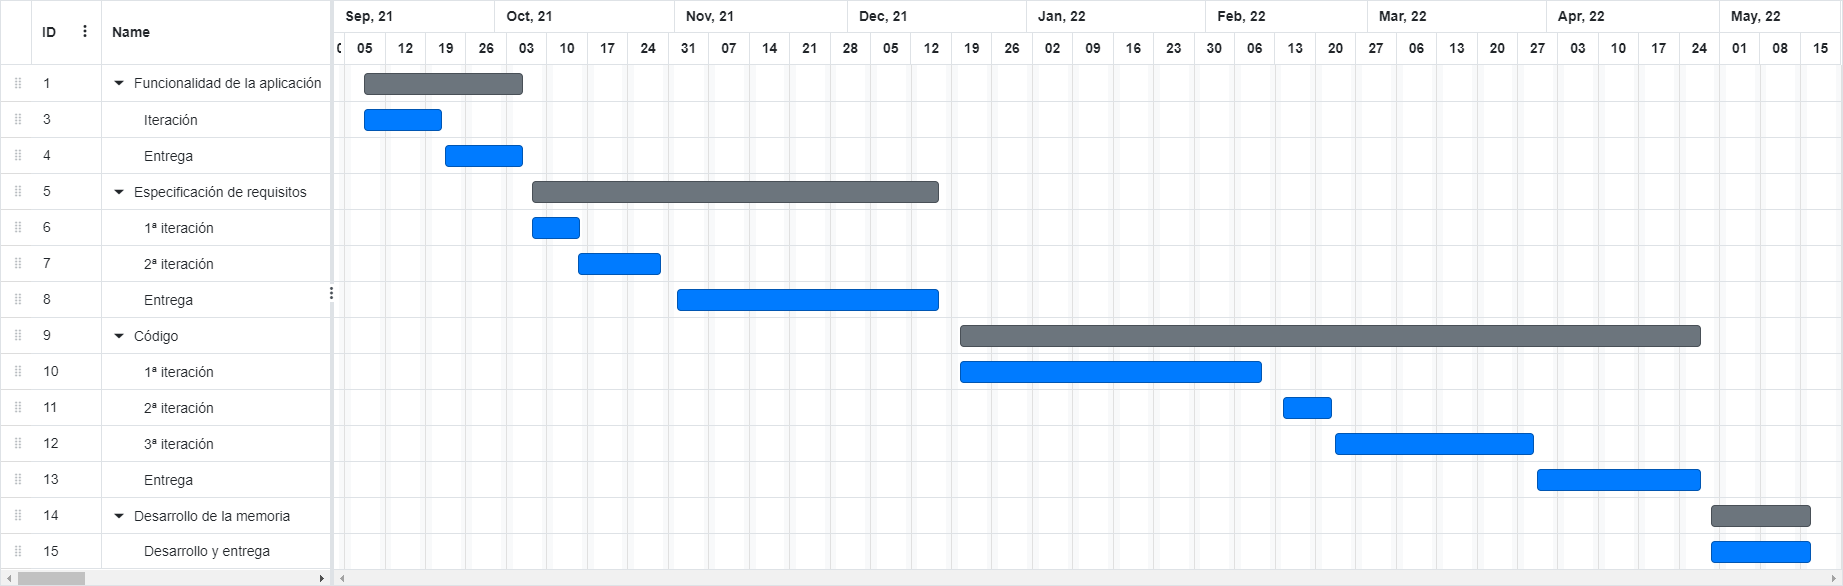
\includegraphics[width=\textwidth]{Images/gantt.png}
    \caption{Gantt chart of project planning}
    \label{fig:gantt}
\end{figure}

During the first phase, the main functionalities of the application were established. Once this phase was completed, the requirements were specified as well as the actors and modules that make up the application. Two iterations were carried out in order to establish the final requirements.

Subsequently, three code iterations were established, in each of which the different modules previously established (login, diet, current diet) were developed. After the code iterations, different white box tests were performed on the different use cases. In the last phase, the memory that complements the code was developed.

In order to carry out the different phases mentioned above, the team held meetings every Saturday, in order to establish the functionality to be developed during the week. At the same time, the meetings helped to know what the team members had done during the previous week, as well as to try to solve together the problems that arose.
\chapter{Conclusiones y trabajo futuro}
\noindent

\section{Conclusiones}
En este proyecto se ha realizado una aplicación que ayuda a gestionar la dieta de un deportista, pudiendo elegir una dieta entre las creadas por otros usuarios. 

Los deportistas pueden crear dietas que posteriormente pueden ser seguidas por otros usuarios. Además los deportistas, tienen la posibilidad de consultar la información detallada de cada uno de los alimentos que deben de consumir durante la realización de la dieta. A su vez, se pueden subir documentos explicativos para que el deportista que sigue la dieta conozca la finalidad cada alimento dentro de la dieta, pudiendo aportar mayor información al usuario.

Se puede valorar la dieta actual para que otros deportistas tenga referencias de ella, pudiendo a su vez, hacer comentarios sobre la dieta seguida.

% A pesar de que los integrantes no habían trabajado previamente con Android, ni habían desarrollado aplicaciones similares para dispositivos móviles, se considera que el servicio desarrollado aporta a los usuarios de la aplicación el valor que se había establecido al principio de la realización del proyecto, cumpliendo con los objetivos planteados al inicio.

En el siguiente enlace se puede ver y descargar, desde el repositorio de GitHub, el código del proyecto así como la aplicación ejecutable: \url{https://github.com/csegundo/Diet-Now}.

\section{Trabajo futuro}
% A continuación se van a describir una serie de implementaciones que se podrían añadir a la aplicación con el objetivo de mejorar la experiencia del usuario durante el uso de la misma.
A continuación se van a describir una serie de ideas de trabajo futuro que se podrían añadir a la aplicación con el objetivo de mejorar la experiencia del usuario durante el uso de la misma.

\begin{itemize}
    % \item \textbf{Modo oscuro:} la aplicación actualmente está implementada con el tema claro, el cual aparece configurado por defecto en numerosas aplicaciones. Son varias las motivaciones que nos pueden llevar a implementar esta mejora, destacando principalmente las siguientes.
    % \begin{enumerate}
    %     \item Comodidad visual: establecer un fondo oscuro en la aplicación como un color negro, gris o azul, disminuye el esfuerzo visual evitando que los ojos sufran de cansancio o fatiga. Además permite que se adapten con mayor facilidad a espacios con poca luminosidad.
    %     \item Ahorro de batería: en la mayoría de dispositivos móviles, el modo oscuro puede ayudar a reducir la batería entre un 14\% y un 60\%, dependiendo del brillo de la pantalla.
    % \end{enumerate}
    
    \item \textbf{Barra inferior de navegación:} el objetivo principal de esta implementación es la mejora de la experiencia del usuario, permitiéndole una navegación más sencilla e intuitiva entre las diferentes vistas añadiendo en la zona inferior de la pantalla un menú con una serie de iconos.% En la Figura \ref{fig:app_bottom_bars} se muestra un \textit{mockup} de dicho menú en dos vistas diferentes de la aplicación.
    % \begin{figure}[H]
    %     \centering
    %     \subfigure[Vista de la dieta actual]{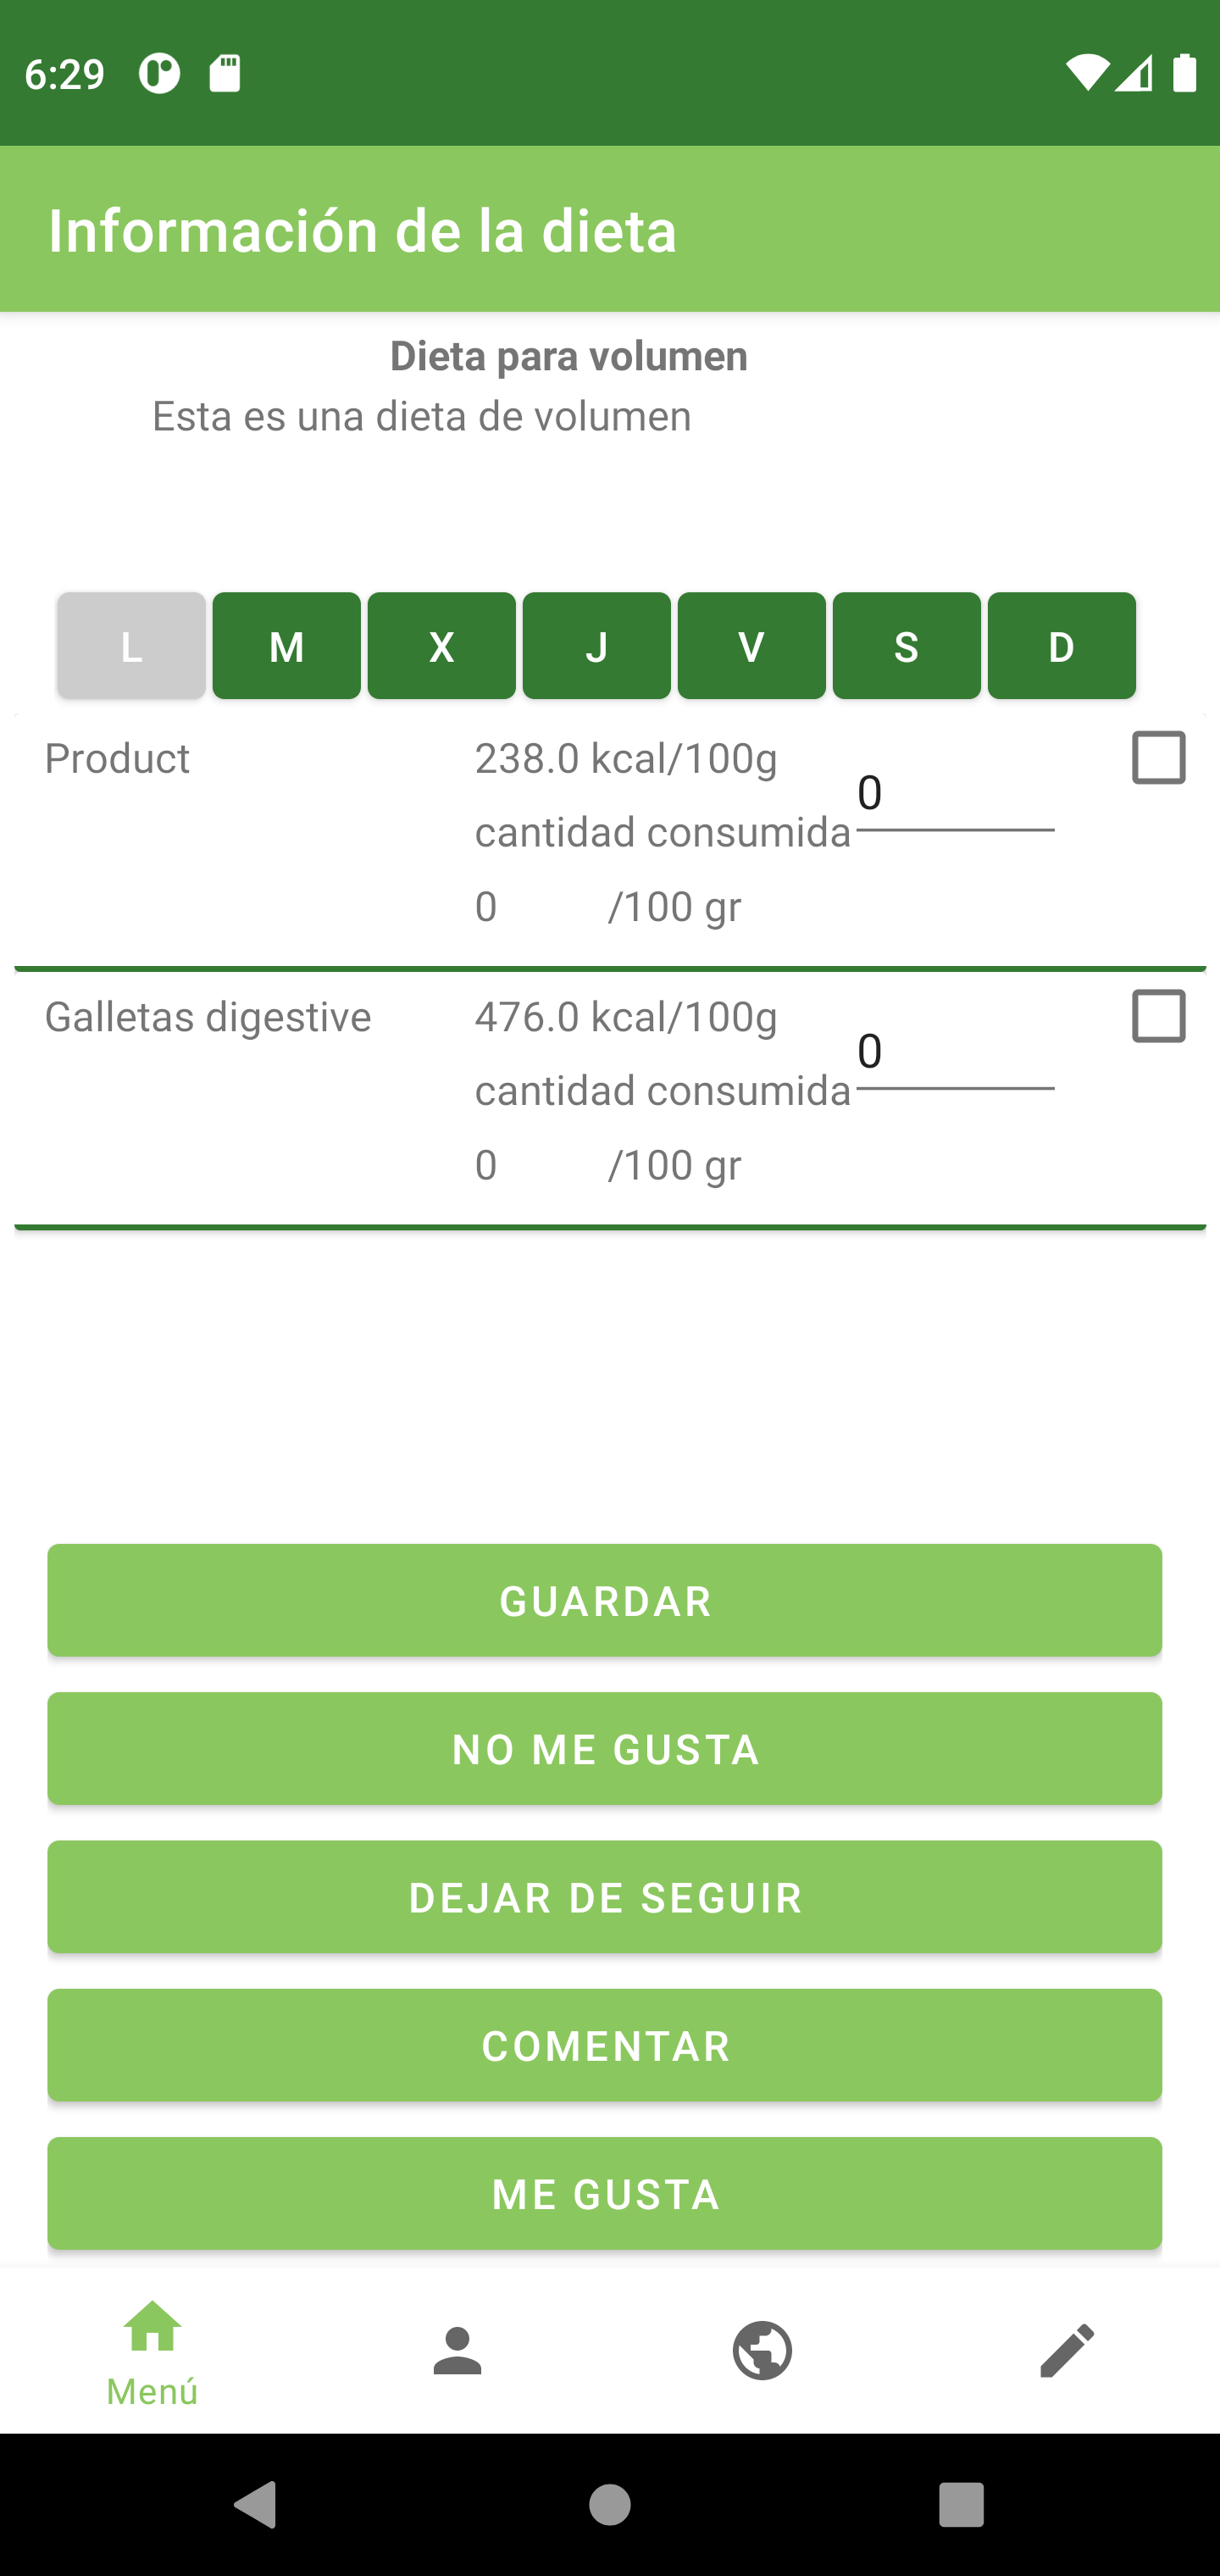
\includegraphics[width=0.45\textwidth]{Images/Capitulo9/bottomBar1.png}}
    %     \subfigure[Vista del perfil del deportista]{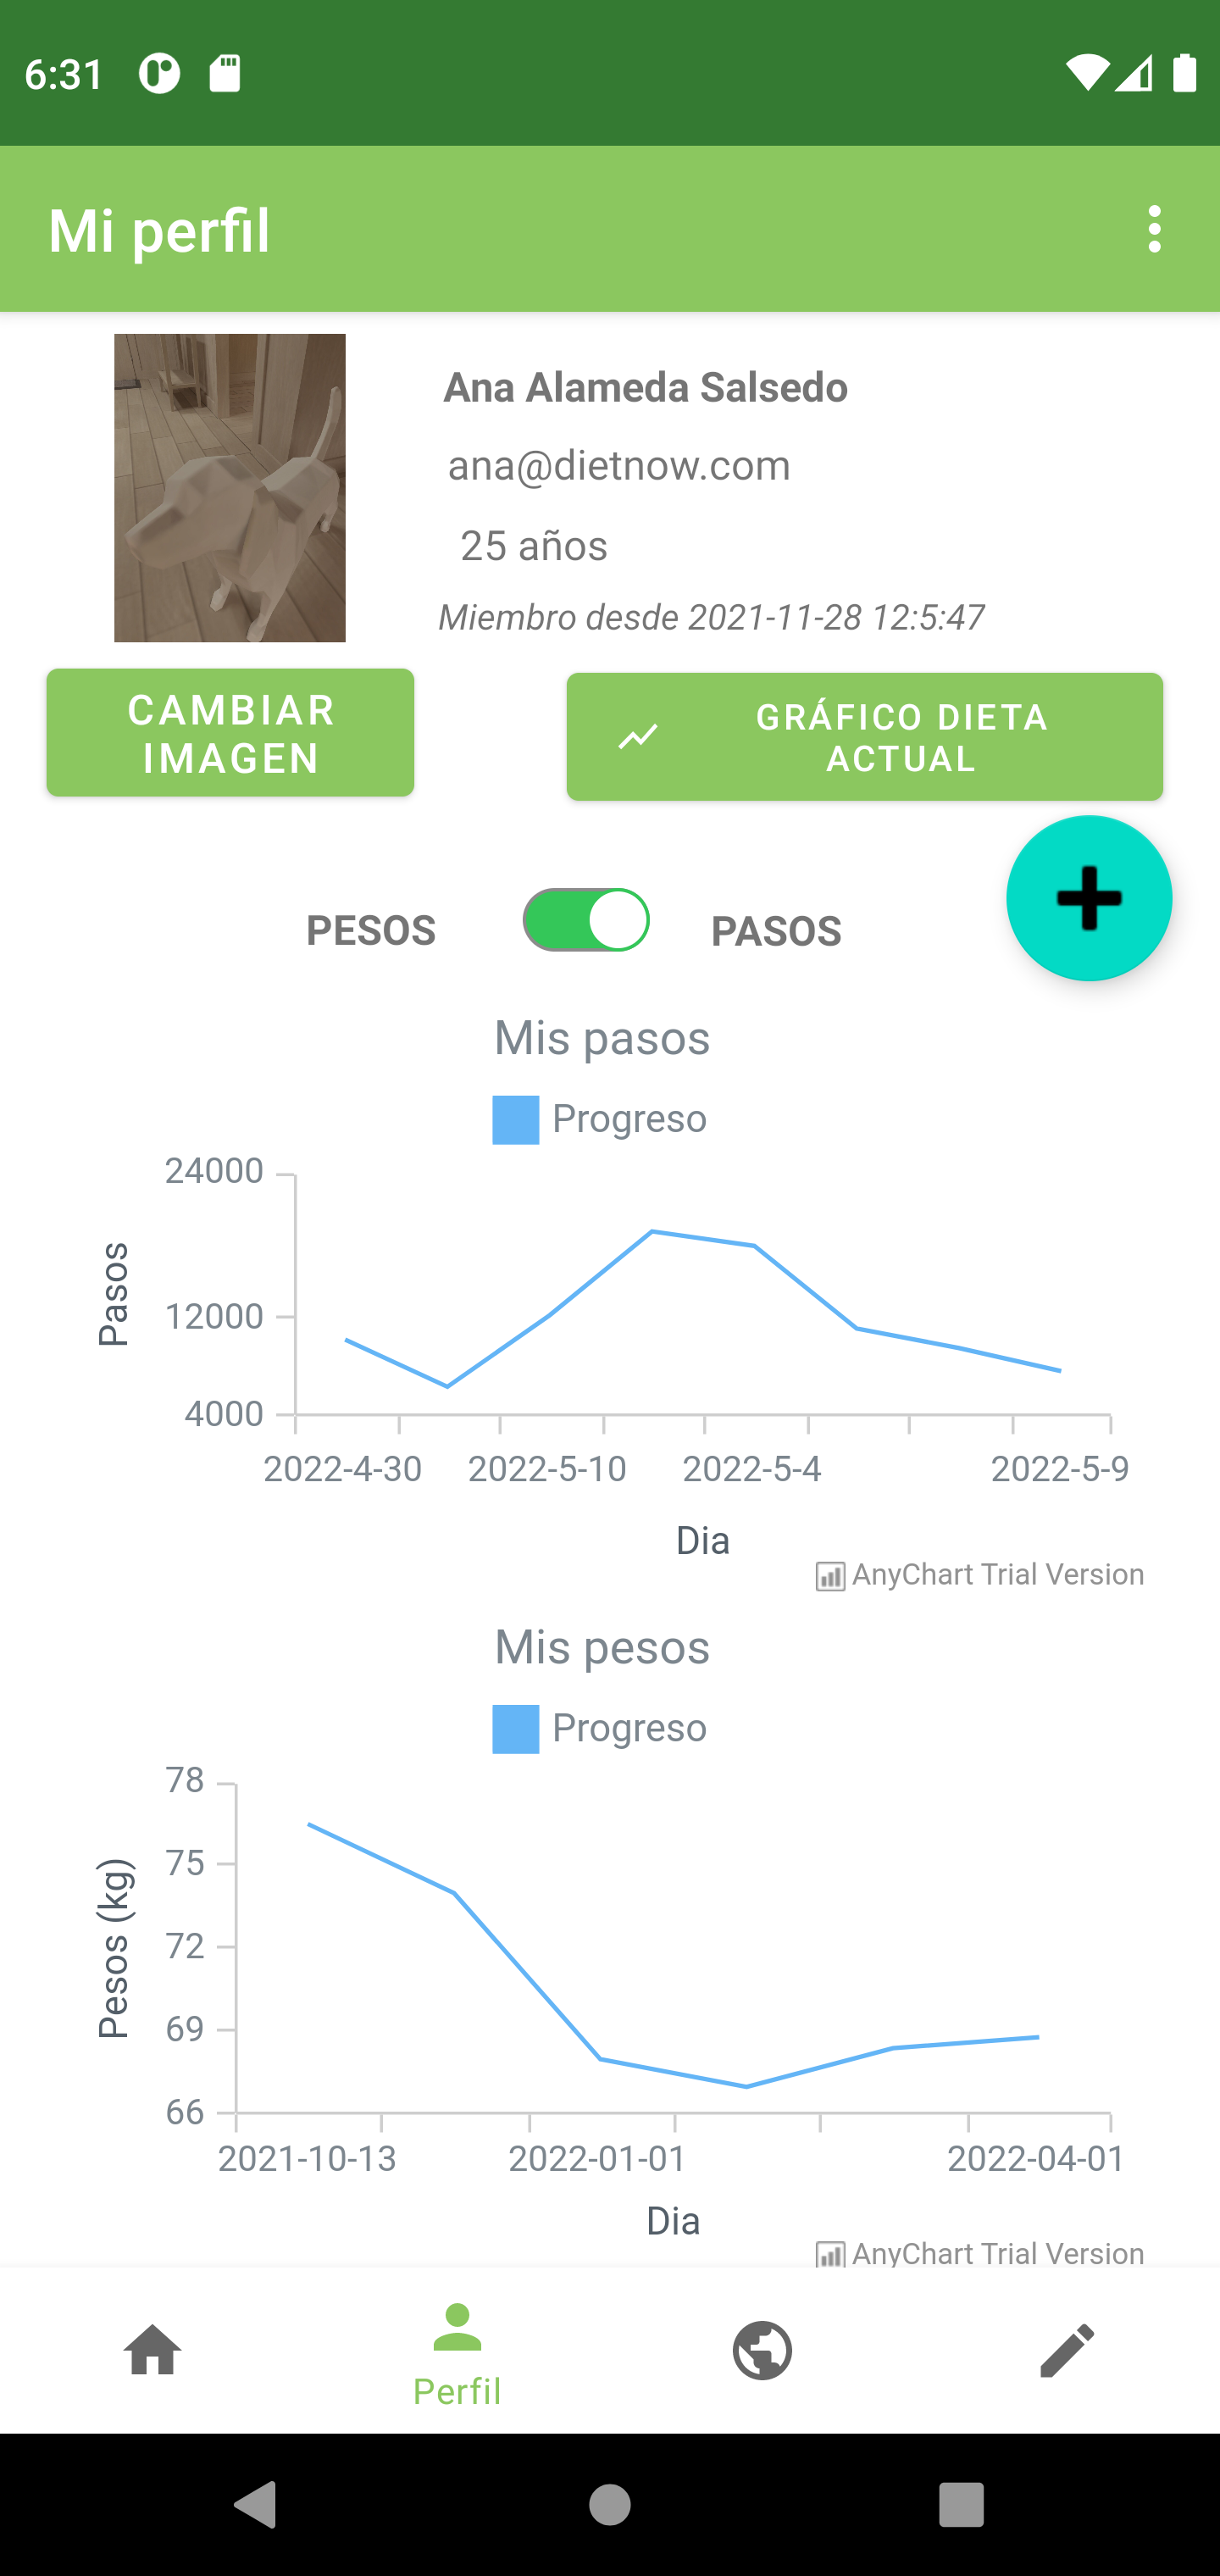
\includegraphics[width=0.45\textwidth]{Images/Capitulo9/bottomBar2.png}}
    %     \caption{\textit{Mockups} del menú inferior en diferentes vistas}
    %     \label{fig:app_bottom_bars}
    % \end{figure}
    
    % \item \textbf{Desplegar los servidores de \textit{Node.js} y \textit{Spring}:} para que la aplicación pueda llegar a todos los públicos, se podría desplegar tanto el servidor de \textit{Node.js} (que se encarga de llamar a la API de \textit{OpenFoodFacts}) como el servidor de \textit{Spring} (encargado de cambiar los campos del módulo de \textit{Firebase Authentication} y explicado anteriormente en la sección \ref{google_firebase_tools}). Una opción sería desplegar estos servidores en \textbf{\textit{Heroku}} \cite{heroku}, una plataforma como servicio (\textit{PaaS}) que nos permitiría realizar llamadas a estas APIs desde cualquier dispositivo ya que se encuentran en la nube y no de forma local.
    
    \item \textbf{Inicio de sesión con una cuenta de Google o Facebook:} para mejorar la usabilidad de la aplicación, se podría implementar esta nueva funcionalidad de inicio de sesión con una cuenta de Google o Facebook. Además del beneficio ya mencionado, podría aumentar considerablemente el número de usuarios en la aplicación debido a que la mayoría de usuarios de Facebook utilizan un dispositivo móvil, como se muestra en la Figura \ref{fig:fb_users}.
    \begin{figure}[H]
        \centering
        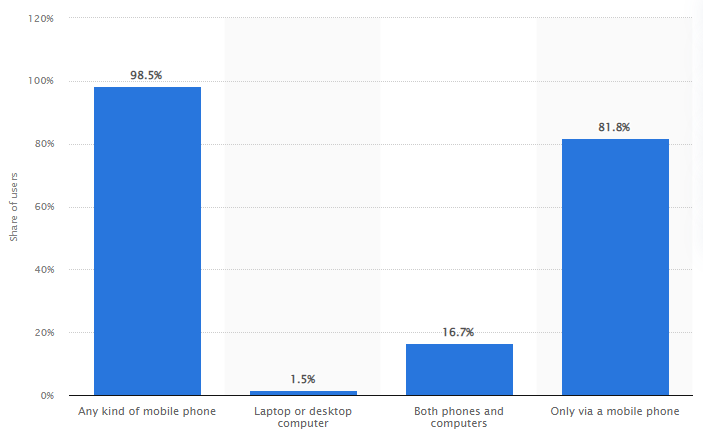
\includegraphics[width=\textwidth]{Images/Capitulo9/fbUsers.png}
        \caption{Dispositivos utilizados para iniciar sesión en Facebook en Enero de 2022 \cite{mobile_max_users}}
        \label{fig:fb_users}
    \end{figure}
    
    \item \textbf{Restablecer contraseña:} actualmente la aplicación no dispone de un sistema de recuperación de contraseña en el caso de que el usuario no recuerde la misma. Esta implementación facilitaría al usuario recuperar el acceso a su cuenta cuando olvida la contraseña, añadiendo un nuevo botón en la pantalla de inicio de sesión que envía un correo electrónico al email del usuario para que éste pueda restablecer la contraseña desde un enlace.
    
    \item \textbf{Añadir alimentos en grupo de comidas:} dar la posibilidad al deportista de añadir alimentos a una dieta en cada una de las cinco comidas que se realizan a lo largo del día. Cuando se va a añadir un alimento a una dieta, el usuario especifica si ese alimento pertenece al desayuno, comida, merienda...
    
    \item \textbf{Compartir dietas:} permitir a los usuarios que usen la aplicación la posibilidad de compartir mediante otras redes sociales o de mensajería las diferentes dietas insertadas en la aplicación.
    
    \item \textbf{Conexión con pulseras inteligentes:} ofrecer la posibilidad al usuario de conectar una pulsera o reloj inteligente a la aplicación. Mediante esta conexión, se pueden recopilar datos como el número de pasos caminados durante el día e introducirlos de forma automática en la cuenta del usuario para que se muestren en la gráfica de los pasos.
    
    \item \textbf{Conectar la gestión de dietas con asistente Alexa o Google:} permitir a los usuarios que deseen crear una dieta la posibilidad de hacerlo mediante voz. Esta herramienta se podría utilizar también para generar una compra mediante el asistente de Alexa o Google con los productos almacenados de una dieta.
    
\end{itemize}
% El comando "\chp" es como el "\chapter" pero mete "Chapter" en vez de "Capitulo"
\chp{9}{Conclusions and future work}
\noindent

% addtocounter: necesario para tener el mismo número de \section que el de español ==> -2 porque hay 2 secciones en el capitulo 9 - igual para las imágenes
\addtocounter{section}{-2}
\addtocounter{figure}{-1}

\section{Conclusions}
In this project we have developed an application that helps to manage the diet of an athlete, being able to choose a diet among those created by other users. 

Athletes can create diets that can later be followed by other users. In addition, athletes have the possibility to consult the detailed information of each of the foods that they should consume during the diet. At the same time, explanatory documents can be uploaded so that the athlete who follows the diet knows the purpose of each food within the diet, being able to provide more information to the user.

The current diet can be evaluated so that other athletes have references of it, being able, in turn, to comment on the diet followed.

% Despite the fact that the members had not previously worked with Android, nor had they developed similar applications for mobile devices, it is considered that the service developed provides the application users with the value that had been established at the beginning of the project, fulfilling the objectives set at the beginning.

In the following link you can view and download, from the GitHub repository, the code of the project as well as the executable application: \url{https://github.com/csegundo/Diet-Now}.

\section{Future work}
% The following is a description of a series of implementations that could be added to the application in order to improve the user's experience while using it.
The following are a number of ideas for future work that could be added to the application in order to improve the user's experience while using the application.

\begin{itemize}
    % \item \textbf{Dark mode:} the application is currently implemented with the clear theme, which is configured by default in many applications. There are several motivations that may lead us to implement this improvement, highlighting mainly the following.
    % \begin{enumerate}
    %     \item Visual comfort: setting a dark background in the application, such as black, gray or blue, reduces eye strain and prevents eye strain and fatigue. It also allows them to adapt more easily to dimly lit spaces.
    %     \item Battery saving: Battery saving: On most mobile devices, dark mode can help reduce battery life by 14\% to 60\%, depending on screen brightness.
    % \end{enumerate}
    
    \item \textbf{Bottom navigation bar:} the main objective of this implementation is to improve the user experience, allowing an easier and more intuitive navigation between the different views by adding a menu with a series of icons at the bottom of the screen.% In Figure \ref{fig:app_bottom_bars_en} a \textit{mockup} of this menu is shown in two different views of the application.
    % \begin{figure}[H]
    %     \centering
    %     \subfigure[View of the current diet]{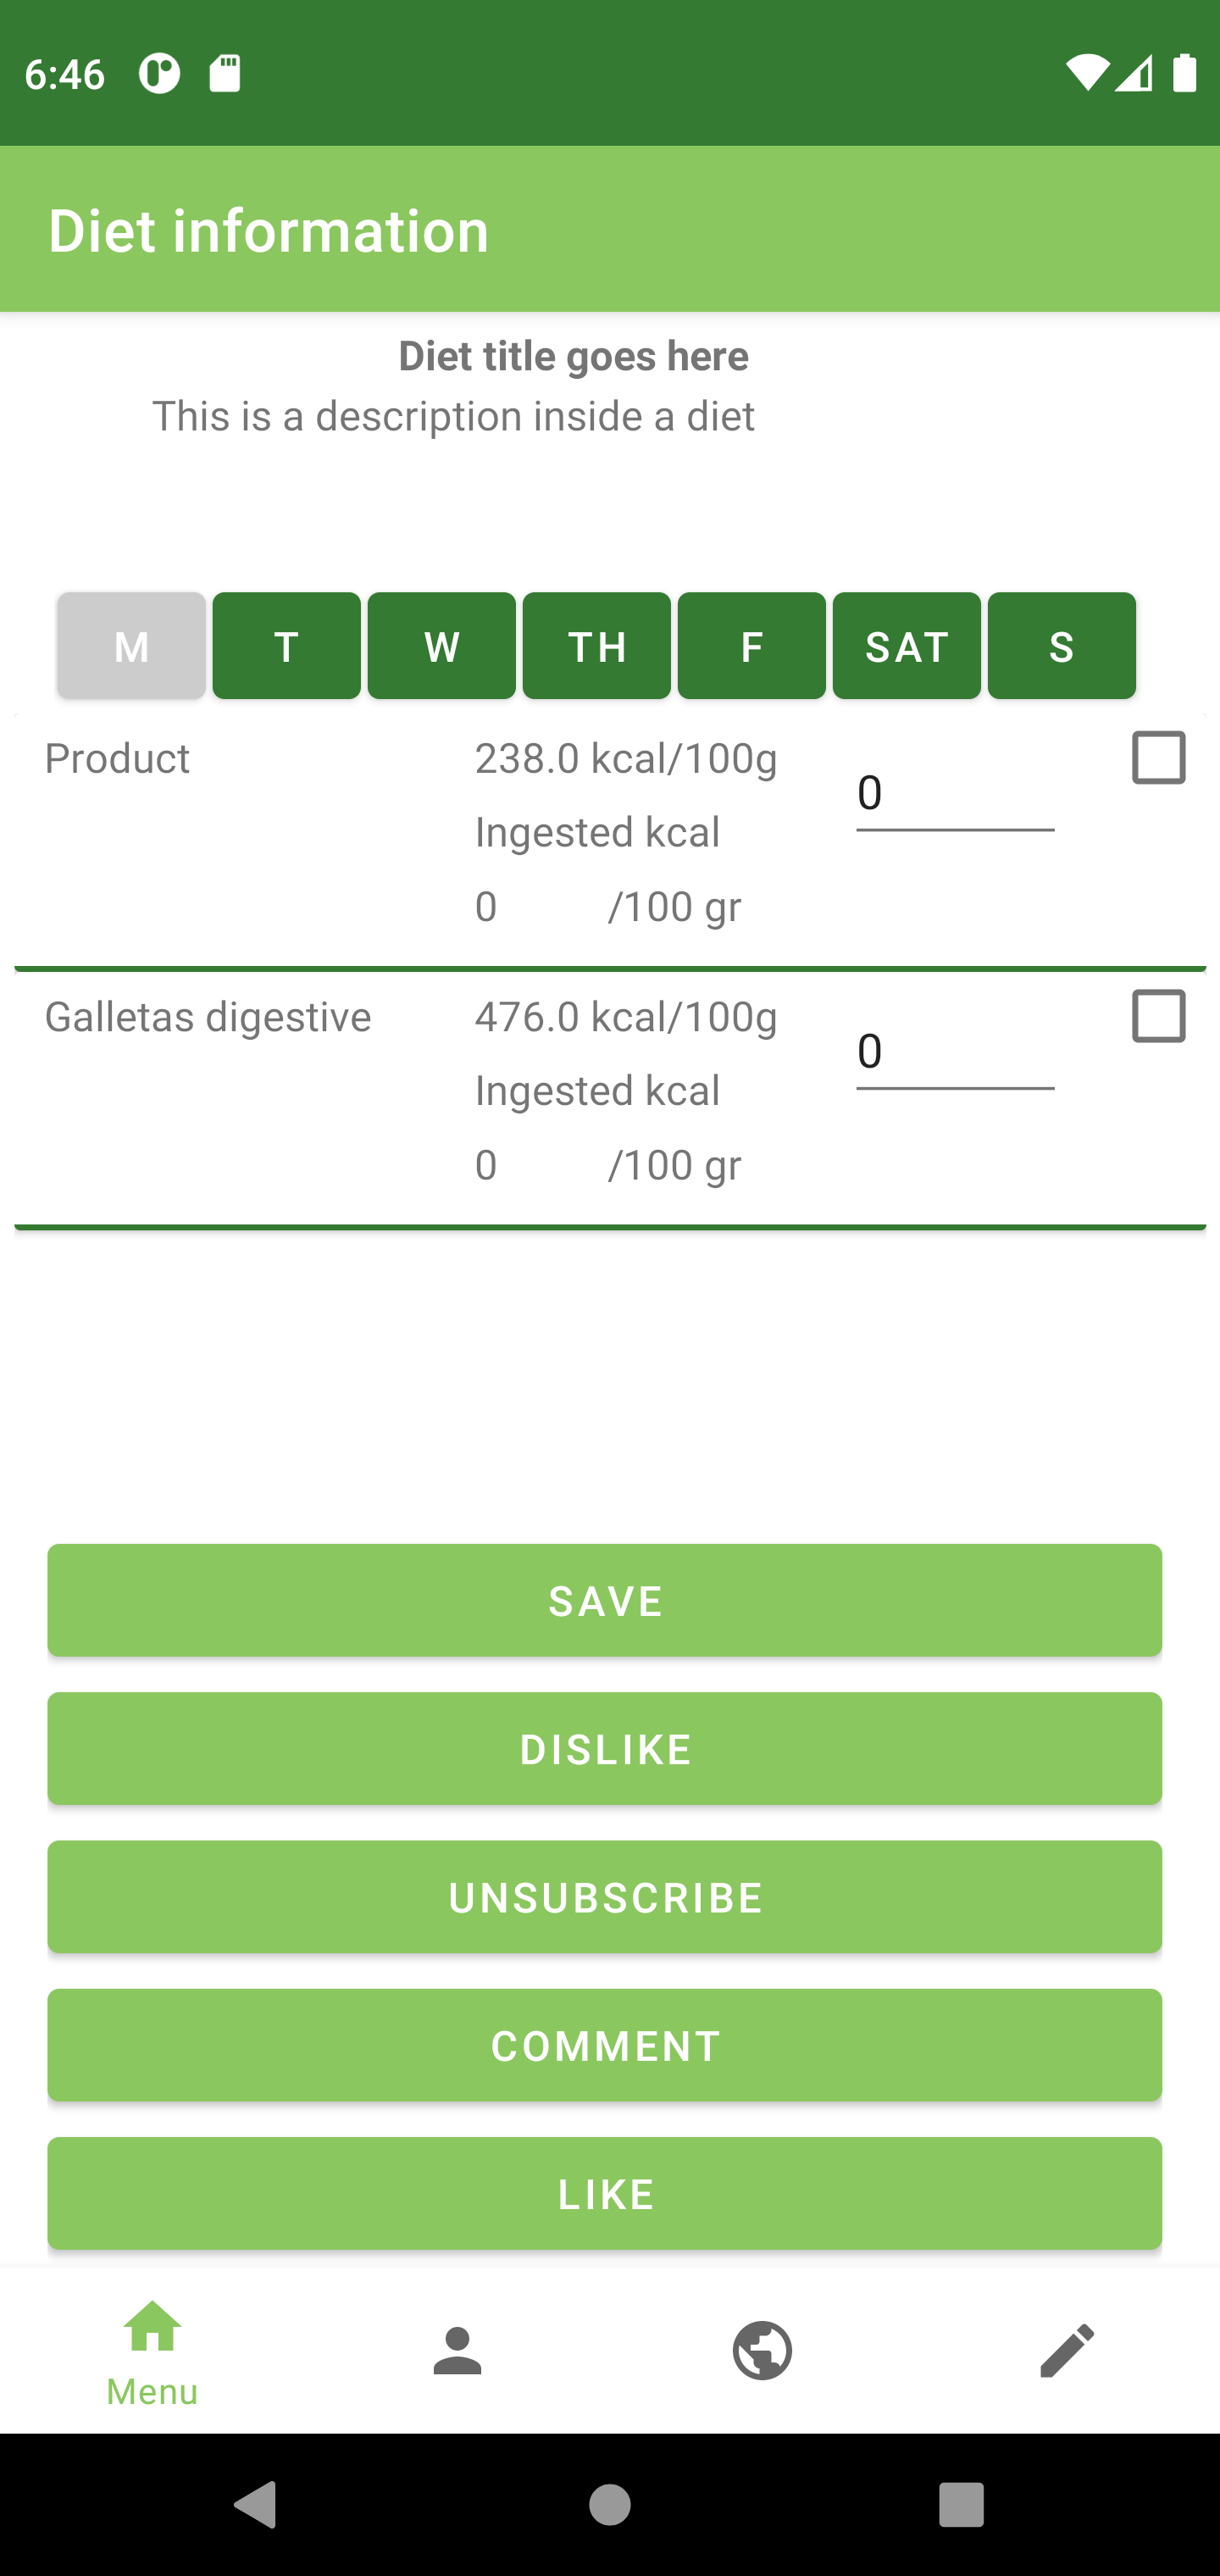
\includegraphics[width=0.45\textwidth]{Images/Capitulo9/bottomBar1_en.png}}
    %     \subfigure[Athlete profile view]{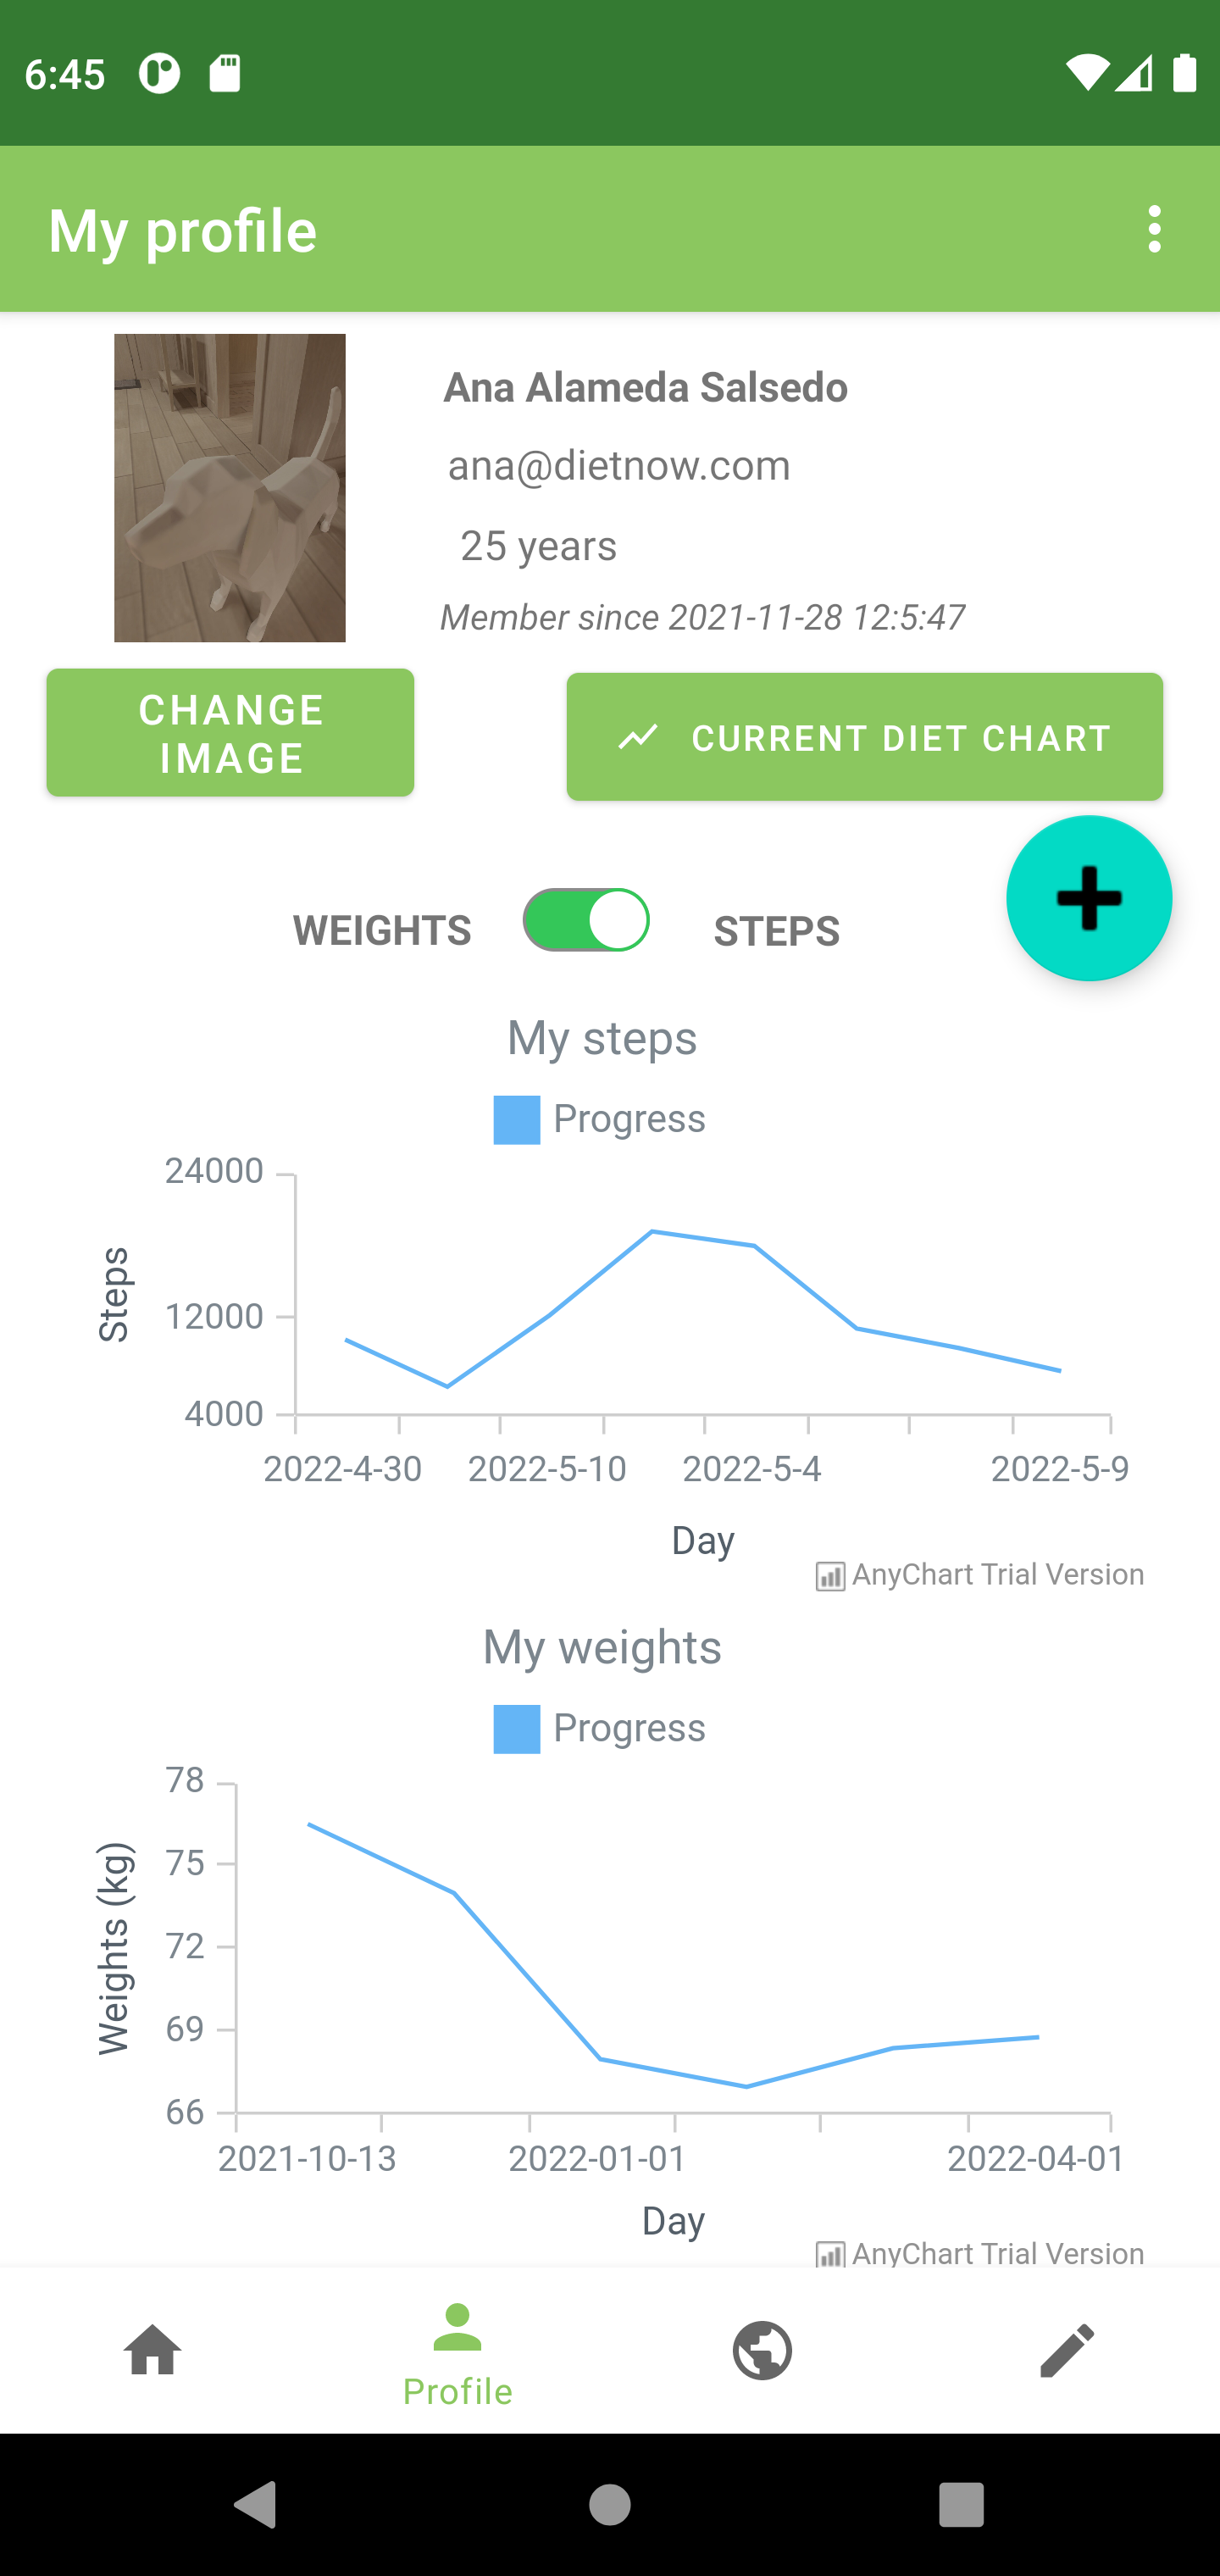
\includegraphics[width=0.45\textwidth]{Images/Capitulo9/bottomBar2_en.png}}
    %     \caption{\textit{Mockups} of the bottom menu in different views}
    %     \label{fig:app_bottom_bars_en}
    % \end{figure}
    
    % \item \textbf{Deploy the servers of \textit{Node.js} and \textit{Spring}:} to enable the application to reach all audiences, it could be possible to deploy both the \textit{Node.js} (which is responsible for calling the API of \textit{OpenFoodFacts}) as the server of \textit{Spring} (in charge of changing the fields of the \textit{Firebase Authentication} module explained above in the section \ref{google_firebase_tools}). One option would be to deploy these servers on \textbf{\textit{Heroku}}, a platform as a service (\textit{PaaS}) that would allow us to make calls to these APIs from any device since they are in the cloud and not locally.
    
    \item \textbf{Signing in with a Google or Facebook account:} to improve the usability of the application, this new functionality of logging in with a Google or Facebook account could be implemented. In addition to the benefit already mentioned, it could considerably increase the number of users in the application due to the fact that most Facebook users use a mobile device, as shown in Fig. \ref{fig:fb_users}.
    \begin{figure}[H]
        \centering
        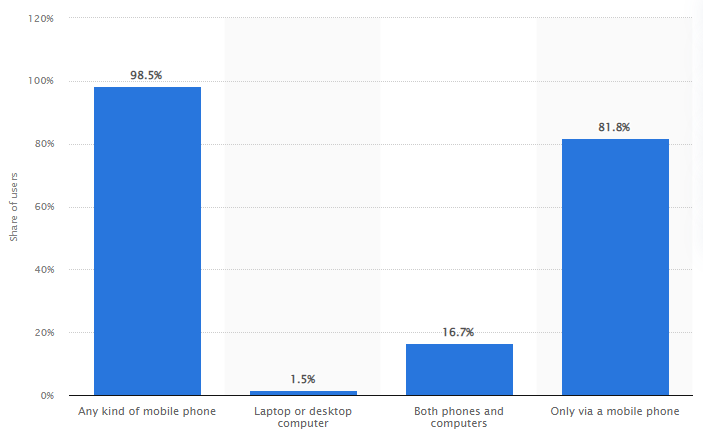
\includegraphics[width=\textwidth]{Images/Capitulo9/fbUsers.png}
        \caption{Devices used to log in to Facebook in January 2022 \cite{mobile_max_users}}
        \label{fig:fb_users}
    \end{figure}
    % https://www.statista.com/statistics/377808/distribution-of-facebook-users-by-device/
    
    \item \textbf{Reset password:} currently the application does not have a password recovery system in case the user does not remember the password. This implementation would make it easier for the user to regain access to their account when they forget their password by adding a new button on the login screen that sends an email to the user's email so that the user can reset the password from a link.
    
    \item \textbf{Adding foods in food groups:} give the athlete the possibility to add food to a diet in each of the five meals that are eaten throughout the day. When a food is to be added to a diet, the user specifies whether that food belongs to breakfast, lunch, afternoon snack...
    
    \item \textbf{Share diets:} allow users who use the application the possibility of sharing through other social or messaging networks all different diets they inserted into the application.
    
    \item \textbf{Connection with smart watches:} offer the possibility for the user to connect a wristband or smartwatch to the application. Through this connection, data such as the number of steps walked during the day can be collected and automatically entered into the user's account to be displayed on the step graph.
    
    \item \textbf{Connect diet management with Alexa or Google assistant:} allow users who create a diet the possibility of doing so by voice commands. This tool could also be used to generate a purchase through the Alexa or Google assistant with the stored products of a diet.
\end{itemize}
\parindent=0em
% El comando "\chp" es como el "\chapter" pero mete "Chapter" en vez de "Capitulo"
\chp{1}{Introduction}

% addtocounter: necesario para tener el mismo número de \section que el de español ==> -2 porque hay 2 secciones en el capitulo 9
\addtocounter{section}{-4}

\pagenumbering{arabic}
\noindent
% \texttt{Lorem ipsum dolor sit amet, consectetuer ad}\\
This chapter will explain the motivation, objectives, work structure and work planning for this project.

\section{Motivation}
% When a person decides to perform any activity with the aim of improving their physical condition, either by increasing or decreasing their weight, they realize that one of the most important factors in achieving this goal is the planning of a healthy and balanced diet.

% For this purpose, complementary tools can be used to carry out this planning, to follow a balanced diet and to plan the different meals during the day.

% With the aim of helping all these users, it has been decided to develop an Android application, in which users will be allowed to follow other diets created. Using this application, the user's eating habits can be improved, keeping a count of calories consumed, understanding food labeling, consulting the nutritional information of the food or even elaborating diets to help the rest of the users.

% introducir el dominio
Every athlete needs to accompany his or her activity with an adequate diet, since nutrition is one of the factors on which physical performance depends. An adequate diet provides the necessary nutrients to maintain an optimal state of health, which translates into performance. Depending on how an athlete eats, you can see how food affects their performance, improving performance and recovery, limiting or even decreasing them, as poor nutrition can promote injuries and fatigue.

% plantear el problema
Currently, there are no mobile applications that can flexibly manage the diets that an athlete needs to follow in order to have a healthy diet that is appropriate to his or her profile. In addition, most of the existing diets on the Internet lack sources or studies that support them and do not have reliable feedback from users who have tried them.

% propuesta que planteamos
To solve these limitations, it has been decided to create an Android application that meets the needs of monitoring and control of diets. It is also possible to see the feedback of the athletes who have followed and evaluated the diet, playing the role of a social network and helping other athletes who are looking for similar goals. In addition, athletes can attach documents to the diets to provide additional information to support them.
\section{Objectives}
The main objective of this project is to develop an Android application that helps athletes to complement their physical activity, following a healthy and balanced diet to achieve the desired physical shape. It is also possible to interact with other athletes, creating diets that can be followed by other athletes or including comments and evaluations in them.

More specific objectives can be defined based on the main objective:
\begin{itemize}
    \item Allow an athlete to register in the application to discover and analyze all the diets in the application, and to update the weight and insert the daily steps, in order to keep a tally and visualize the progress in graphs.
    \item Allow athletes to follow a diet inserted from the application by any of the users, whether they are athletes or administrators.
    \item To offer the possibility to the athlete to evaluate the diet he/she is following, in order to help other athletes to decide and know which diets are being effective.
    \item Allow all athletes the ability to create one or more diets, detailing the foods that compose it, the recommended amount of each one of them and even publishing documentation that helps to follow the diet.
    \item Allow athletes to add foods to diets and have their nutritional information updated at all times.
\end{itemize}
\section{Organización de la memoria}
A continuación se describe de manera breve la estructura de la memoria:

\begin{itemize}
    \item \textbf{Capítulo 1:} en este capítulo se describe la motivación del trabajo, los objetivos y la estructura de la memoria.
    \item \textbf{Capítulo 2:} en este capítulo se estudian herramientas similares a la que se ha realizado en el trabajo.
    \item \textbf{Capítulo 3:} en este capítulo se describe la tecnología utilizada para implementar el proyecto.
    \item \textbf{Capítulo 4:} en este capítulo se definen los actores y casos de uso que se explicarán mediante tablas junto a sus requisitos.
    \item \textbf{Capítulo 5:} en este capítulo se explica el diagrama entidad relación en el que se ha basado el proyecto y la implementación de la base de datos.
    \item \textbf{Capítulo 6:} en este capítulo se explica la arquitectura de la aplicación y los patrones utilizados.
    \item \textbf{Capítulo 7:} en este capítulo se realiza un estudio sobre el diseño e implementación de los casos de uso más relevantes.
    \item \textbf{Capítulo 8:} en este capítulo se exponen las estadísticas aportadas por usuarios que han dado su opinión sobre el producto.
    \item \textbf{Capítulo 9:} en este capítulo se enumeran los casos de uso que se harán en un futuro explicándolos brevemente.
    \item \textbf{Capítulo 10:} en este capítulo se expone el trabajo realizado por cada uno de los autores.
    \item \textbf{Anexo I:} manual de usuario.
    \item \textbf{Anexo II:} preguntas de evaluación.

\end{itemize}

\section{Planning}
This part describes all the planning carried out during the development of this project, detailing the different meetings and iterations performed. In figure  \ref{fig:gantt} the following \textbf{\textit{Gantt}} diagram can be seen where the different phases of the project are indicated.
\begin{figure}[H]
    \centering
    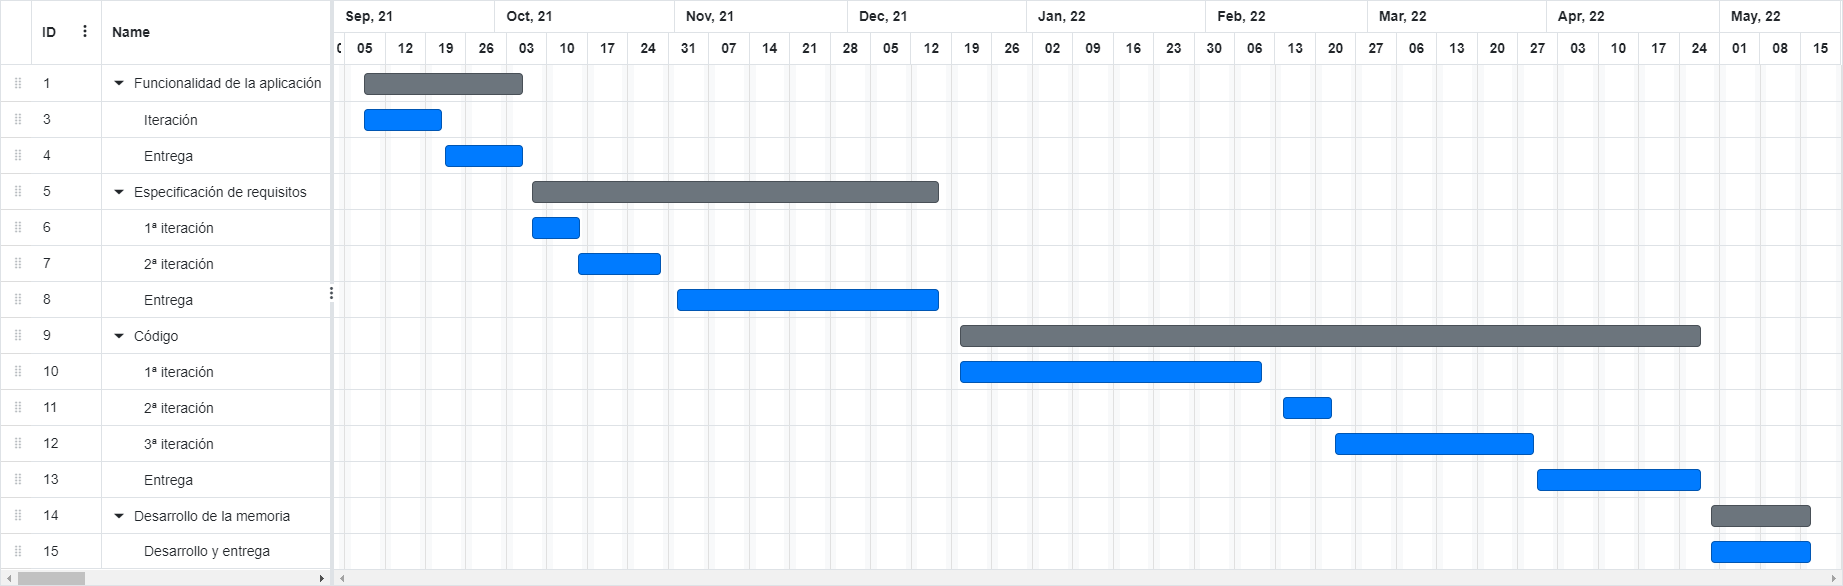
\includegraphics[width=\textwidth]{Images/gantt.png}
    \caption{Gantt chart of project planning}
    \label{fig:gantt}
\end{figure}

During the first phase, the main functionalities of the application were established. Once this phase was completed, the requirements were specified as well as the actors and modules that make up the application. Two iterations were carried out in order to establish the final requirements.

Subsequently, three code iterations were established, in each of which the different modules previously established (login, diet, current diet) were developed. After the code iterations, different white box tests were performed on the different use cases. In the last phase, the memory that complements the code was developed.

In order to carry out the different phases mentioned above, the team held meetings every Saturday, in order to establish the functionality to be developed during the week. At the same time, the meetings helped to know what the team members had done during the previous week, as well as to try to solve together the problems that arose.

%%%%%%%%%%%%%%%%%%%%%%%%%%%%%%%%%%%%%%%%%%% Parte 3 - BIB y licencia
\biblioTFG{11}
\printglossaries

\parte{B}{Anexos}
% % RESETEAR LOS CONTADORES PARA LOS ANEXOS
\setcounter{chapter}{1}
\setcounter{section}{0}
%%%%%%%%

\anx{I}{Guía de instalación}
\noindent
La aplicación en su conjunto, como se ha mencionado en anteriores puntos de esta memoria, consta de varios sistemas, desde la lógica de la aplicación hasta las llamadas a las diferentes APIs que ésta usa.

Para cada uno de estos sistemas, es necesario una configuración y despliegue específicos, es por ello que en este anexo se muestra cómo proceder a desplegar todos los entornos necesarios para el correcto funcionamiento de la aplicación.

\section{Instalación y despliegue del servidor Spring Boot}
Como ya se mencionó en el capítulo \ref{spring_boot_tool}, las peticiones que los administradores mandan a los endpoints de la API en Spring se utilizan tanto para la creación de nuevos usuarios como para realizar cambios en el correo electrónico y/o contraseña de éstos.

% AÑADIR AQUI REFERENCIAS A LA BIBLIOGRAFIA DE MAVEN Y GRADLE
En primer lugar cabe destacar que para desplegar el servidor de Spring se puede utilizar Maven o Gradle.\\
\textbf{\textit{Maven}} \cite{maven} ha sido y es una de las herramientas más populares para la gestión y construcción de proyectos en Java, utilizando conceptos provenientes de Apache Ant. La configuración de un proyecto utilizando Maven se basa en un fichero \texttt{.xml} en el cual se declaran los diferentes requerimientos (como las dependencias) para la construcción.\\
Por otro lado, \textbf{\textit{Gradle}} \cite{gradle} es una herramienta de automatización de compilación de código abierto que no emplea lenguaje XML como Maven, sino que se basa en un lenguaje específico del dominio (DSL) basado en Groovy \cite{groovy}.\\
Existen algunas diferencias entre Maven y Gradle, como el tiempo de construcción que en Gradle es más corto y rápido que en Maven; o los scripts, Maven utiliza XML lo que hace que los scripts sean más largos en comparación con los de Gradle, que son más cortos y limpios. Son estas las razones principales por las que se ha decidido emplear Gradle para la compilación, por lo que las instrucciones se realizarán basándose en la utilización de Gradle.

Para proceder al despliegue de este servidor es necesario tener localmente el proyecto de Spring, que se puede conseguir clonando el repositorio de este proyecto. Posteriormente, es necesario tener instalada la versión más reciente de Gradle y se deberá de añadir a las variables de entorno.\\
Luego se deben de añadir las dependencias necesarias de Google Firebase para el correcto funcionamiento, quedando un script similar al mostrado en la Figura \ref{fig:gradle_script}.

\begin{figure}[H]
    \centering
    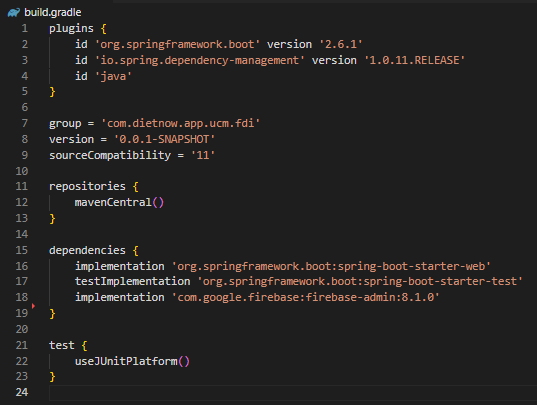
\includegraphics[width=0.8\textwidth]{Images/Annexes/gradle.png}
    \caption{Script de Gradle}
    \label{fig:gradle_script}
\end{figure}

Para compilar y ejecutar el servidor de Spring se deberá ejecutar el comando ``\texttt{gradlew bootRun}``, el cuál mostrará una salida como la de la Figura \ref{fig:gradle}:
\begin{figure}[H]
    \centering
    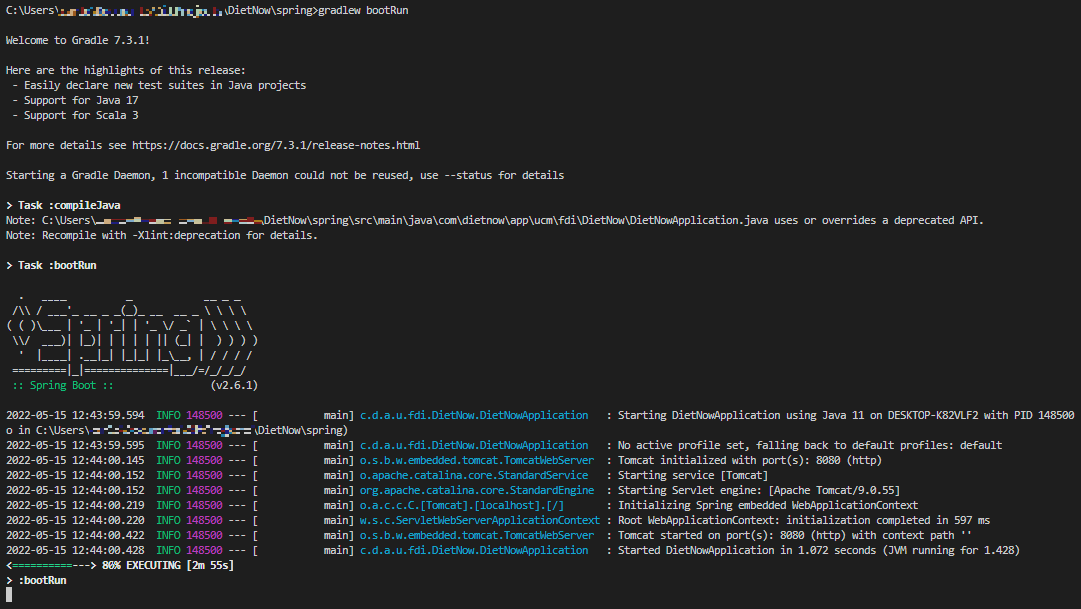
\includegraphics[width=\textwidth]{Images/Annexes/gradle_commandline.png}
    \caption{Ejecución de Gradle}
    \label{fig:gradle}
\end{figure}



\section{Instalación y despliegue del servidor Node.js}
El despliegue de este servidor es necesario para poder obtener la información nutricional de los diferentes alimentos dado el código de barras del mismo.

% AÑADIR AQUI REFERENCIAS A LA BIBLIOGRAFIA DE NODE
Para poder ejecutar y desplegar este servidor, es necesario tener instalada una versión actualizada de Node.js. En este caso no es necesaria ninguna dependencia externa adicional ya que las peticiones que se solicitan a la API de Open Food Facts se realizan mediante el módulo \texttt{https} ya implementado en Node.js por defecto. Para tener de forma local este proyecto de Node.js, se puede conseguir clonando el repositorio de este proyecto.

Posteriormente y, en la raíz del proyecto de Node.js, se deberá de ejecutar por línea de comandos en la terminar el comando ``\texttt{node index.js}``.\\
Para comprobar el correcto despliegue, se puede realizar una petición a esta API accediendo a la url ``\texttt{http://localhost:3000/dietnow/api/product/?barcode=XXXXXXXX}`` en el navegador para obtener la información nutricional del producto solicitado mediante el código de barras especificado, produciendo una salida similar a la mostrada en la Figura \ref{fig:node}.

\begin{figure}[H]
    \centering
    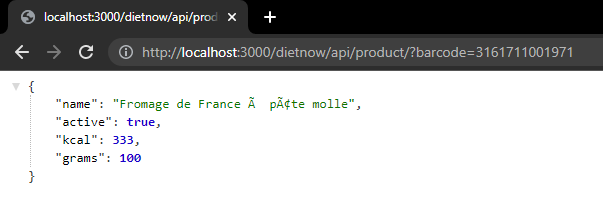
\includegraphics[width=\textwidth]{Images/Annexes/node.png}
    \caption{Producto solicitado a la API de Node.js}
    \label{fig:node}
\end{figure}
% RESETEAR LOS CONTADORES PARA LOS ANEXOS
\setcounter{chapter}{2}
\setcounter{section}{0}
\setcounter{figure}{0}
%%%%%%%%

\anx{I}{Guía del usuario}
\noindent
Una vez instalada y abierta la aplicación se hace visible el menú de inicio de sesión se puede iniciar sesión o registrarse. Como se muestra en el figura \ref{fig:vista_registrarse}, en caso de disponer de una cuenta ya creada se introduce el correo electrónico y la contraseña con la que se creó la cuenta para iniciar sesión y en caso de no tener cuenta el botón ``Registrarse`` ofrece la posibilidad de rellenar un formulario y crear así una cuenta.

\begin{figure}[H]
    \centering
    \subfigure[Vista de iniciar sesión]{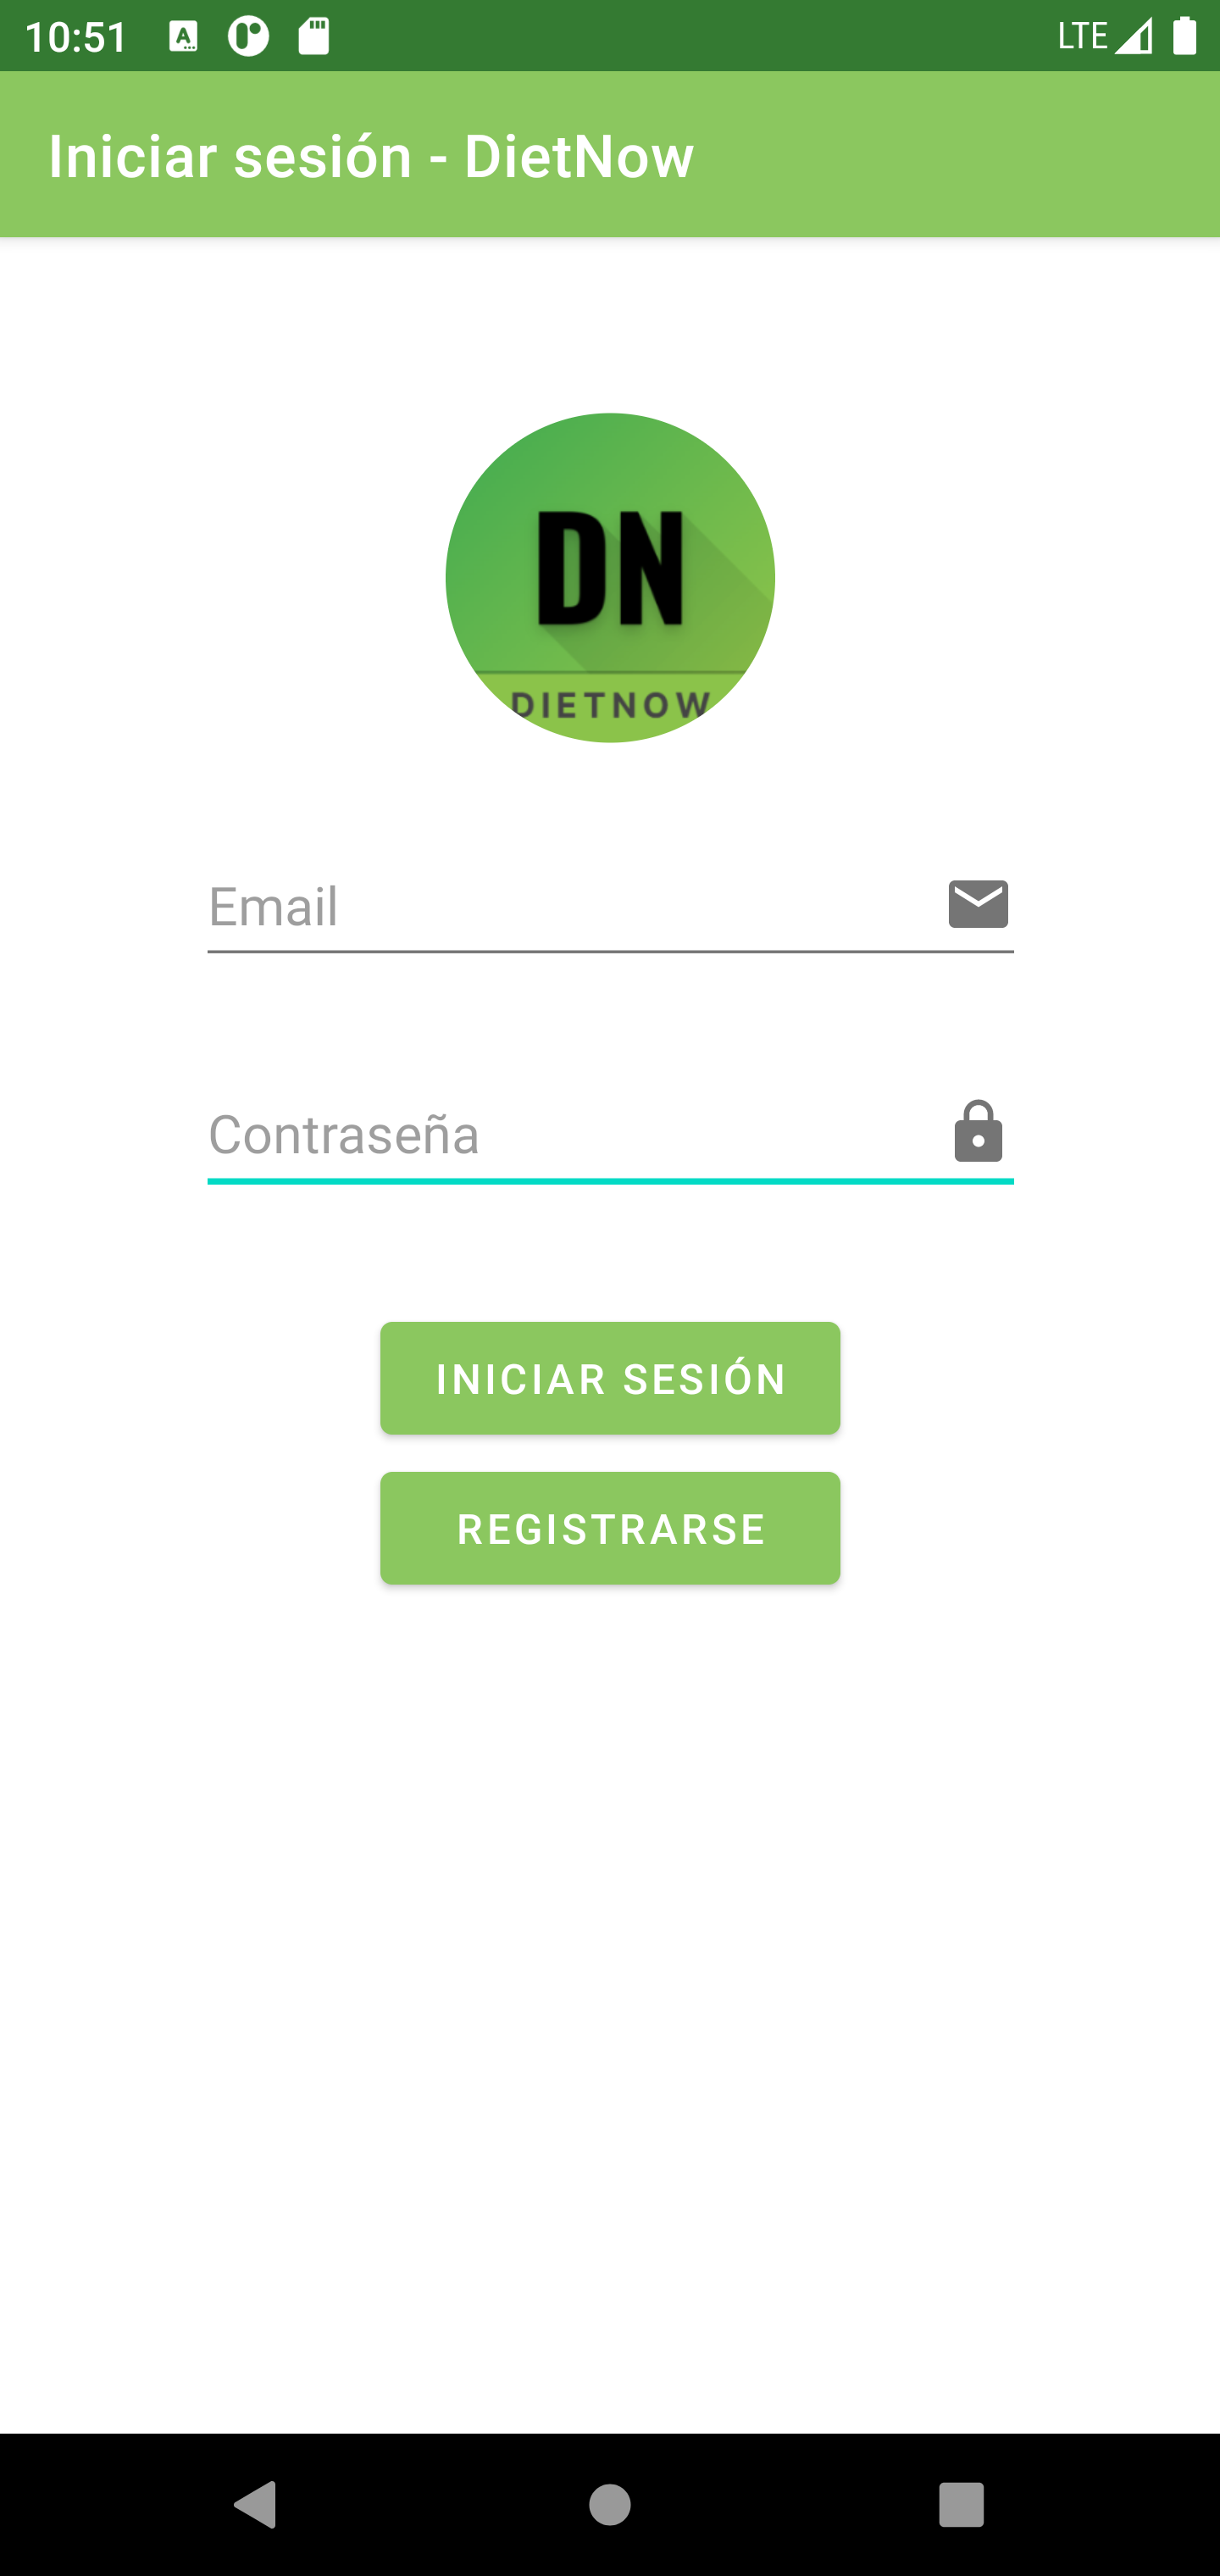
\includegraphics[width=0.4\textwidth]{Images/Annexes/Iniciar_sesion.png}}
    \subfigure[Vista de registro]{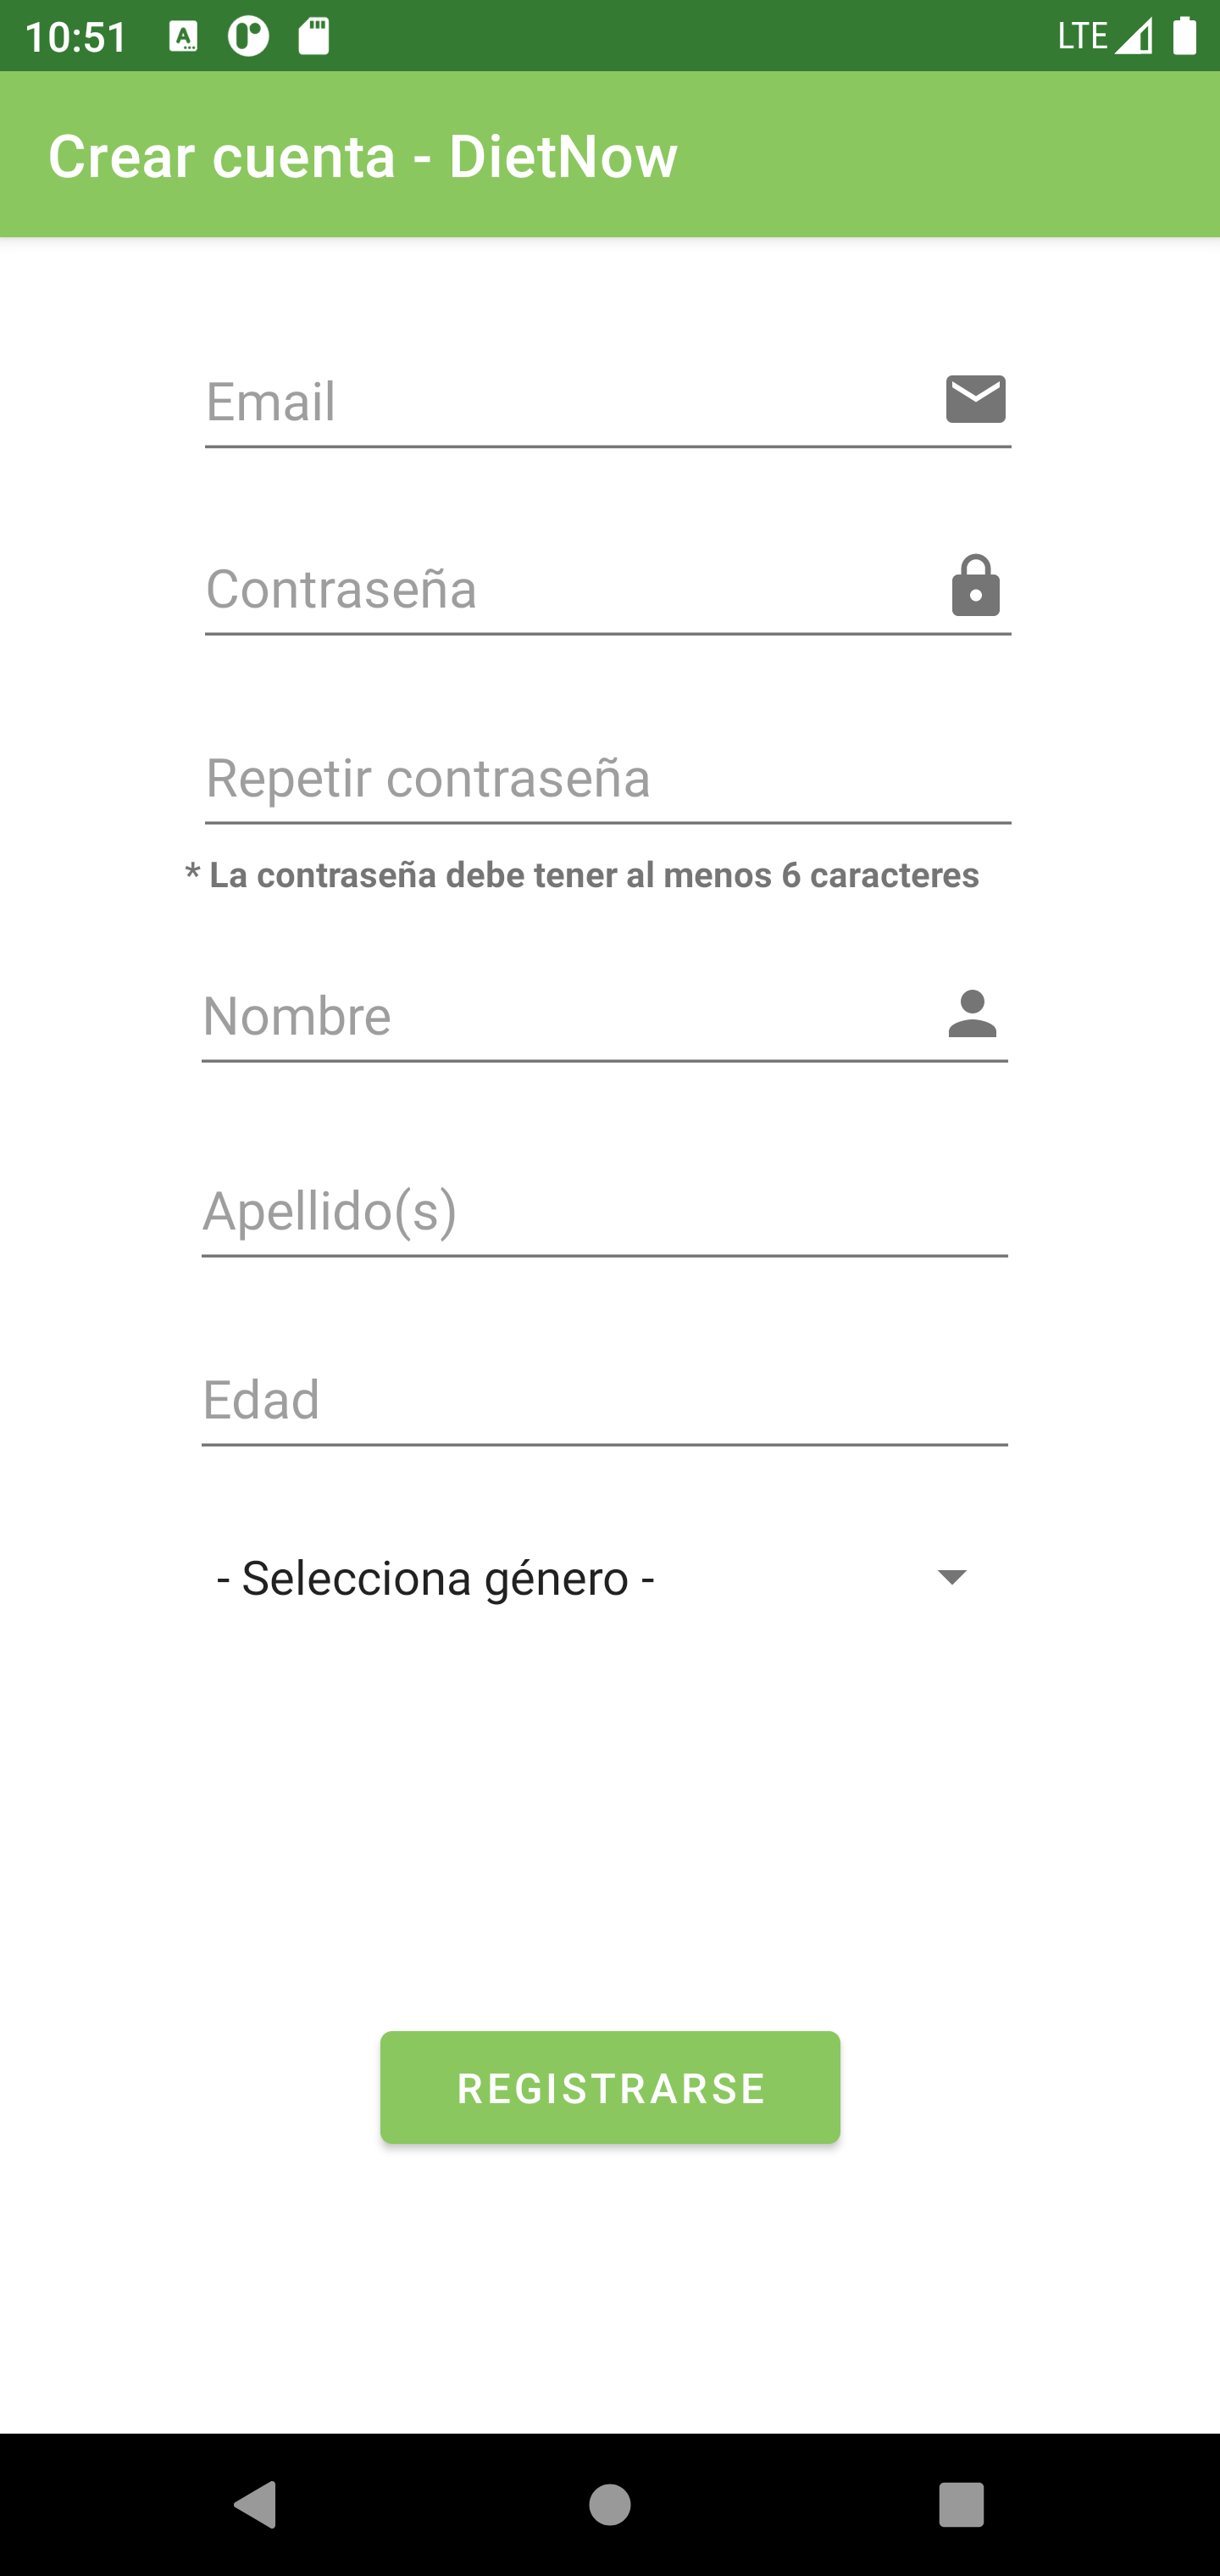
\includegraphics[width=0.4\textwidth]{Images/Annexes/Registrarse.png}}
    \caption{Vistas de la aplicación}
    \label{fig:vista_registrarse}
\end{figure}

Cuando se accede a la aplicación lo primero que aparece es el menú principal \ref{fig:vista_principal}, que en función del rol que tenga el usuario verá más o menos opciones, desde este menú se puede acceder a todas las funcionalidades de la aplicación siempre y cuando se tengan los permisos para ello. Los roles son Usuario y Administrador.

\begin{figure}[H]
    \centering
    \subfigure[Menú principal deportistas]{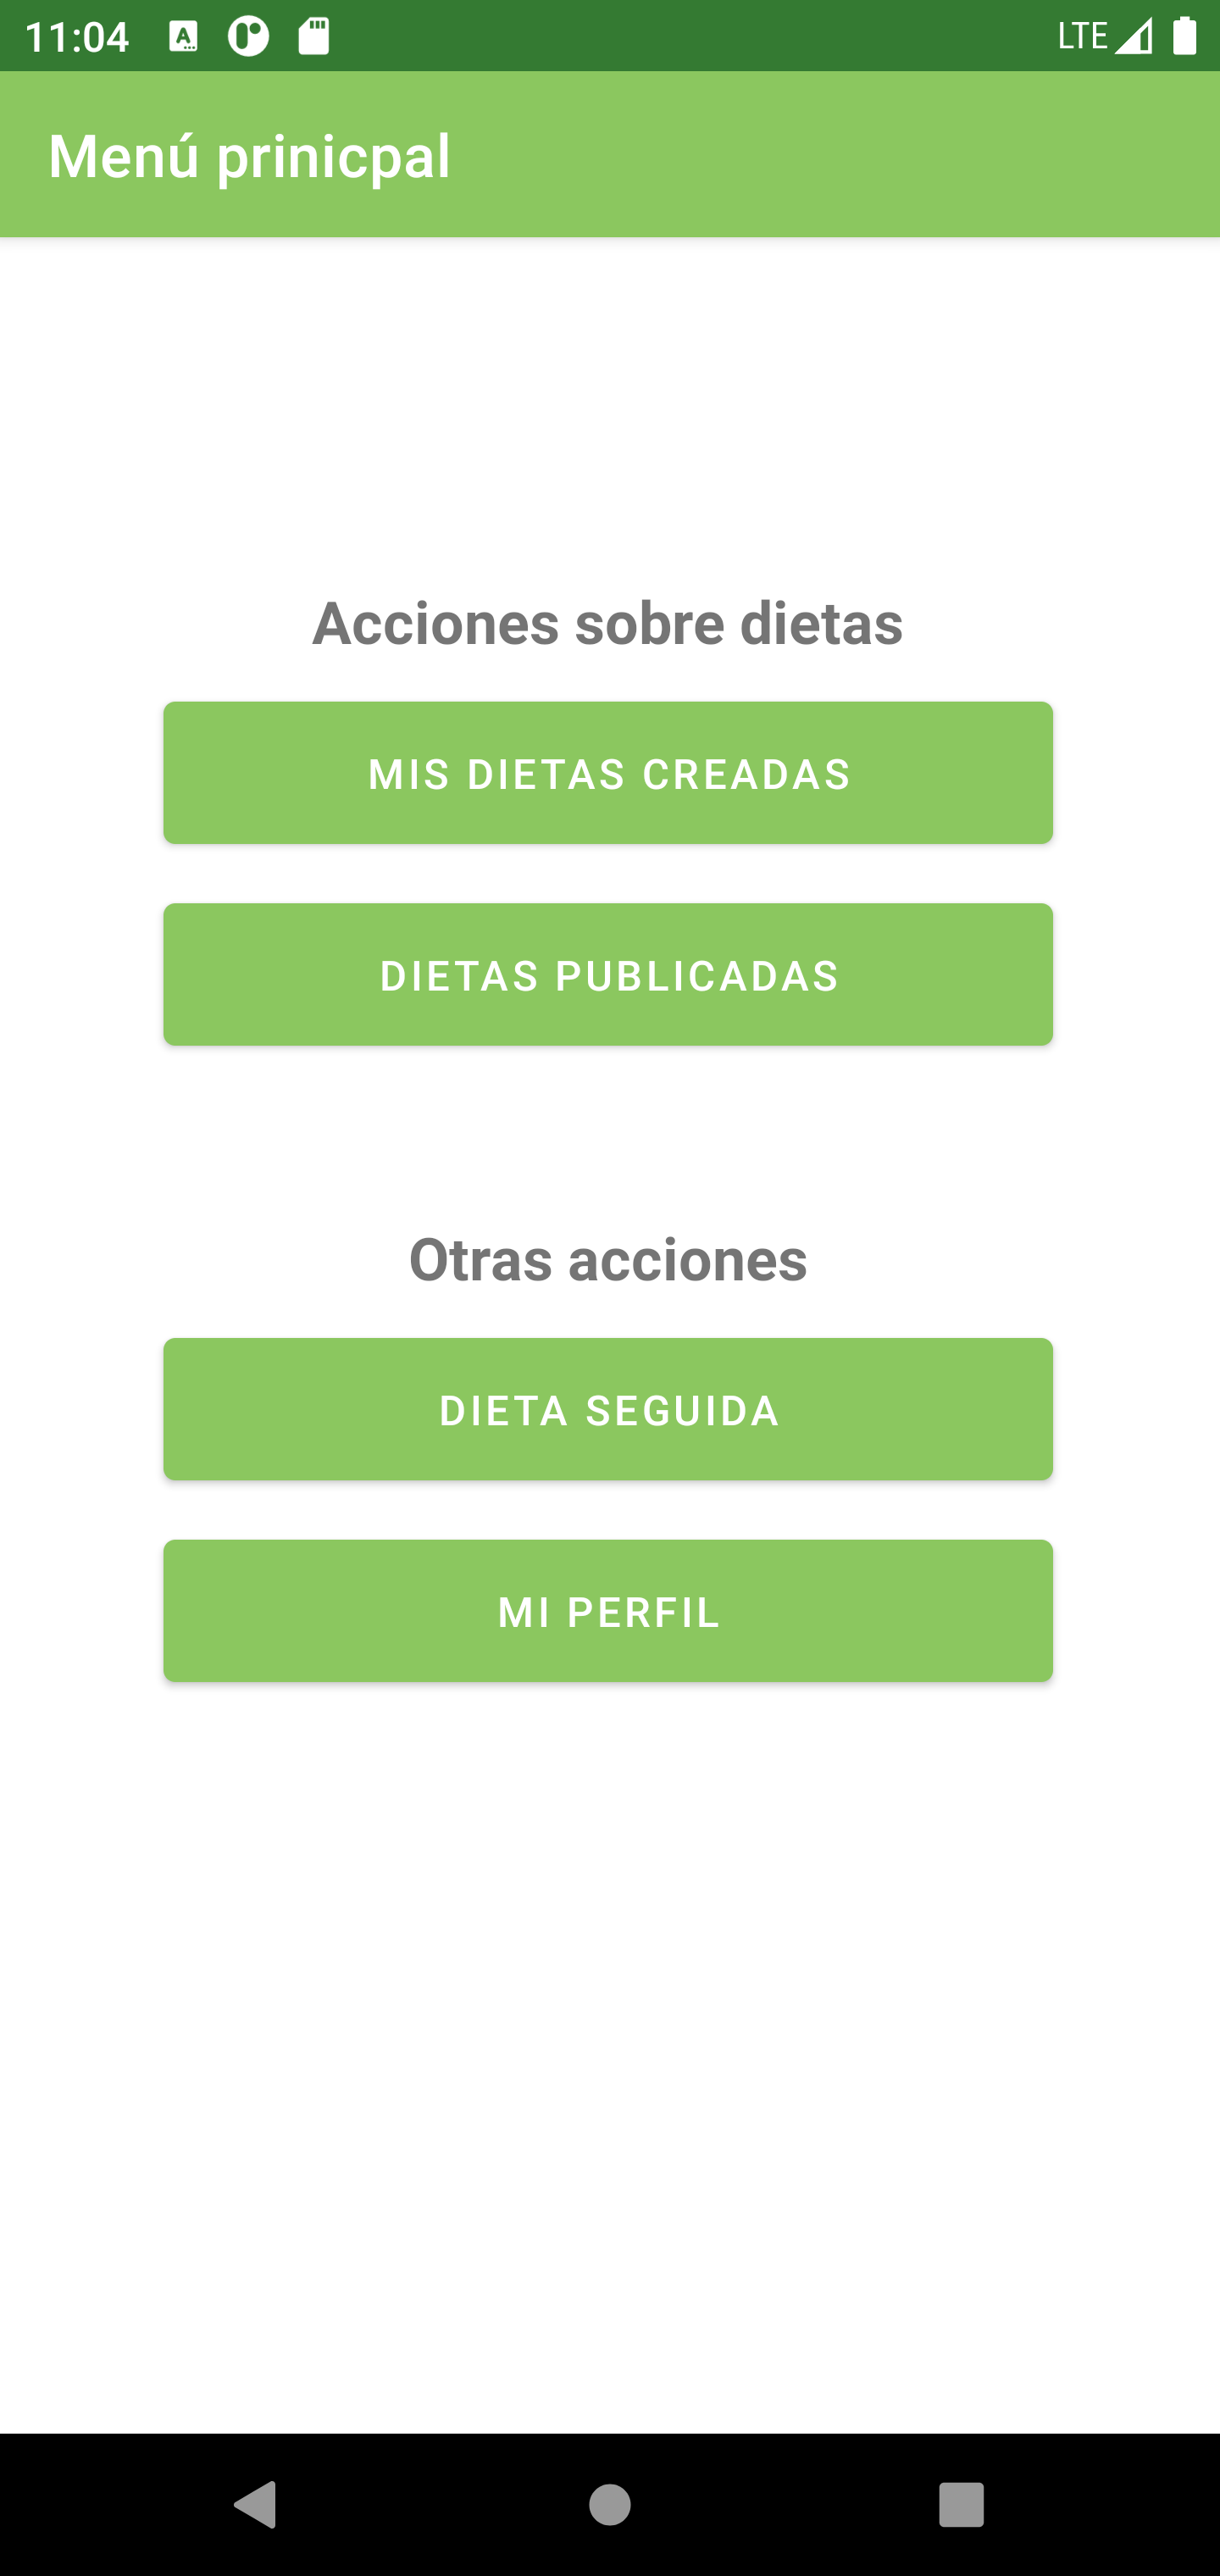
\includegraphics[width=0.4\textwidth]{Images/Annexes/Menu_usuarios.png}}
    \subfigure[Menú principal administradores]{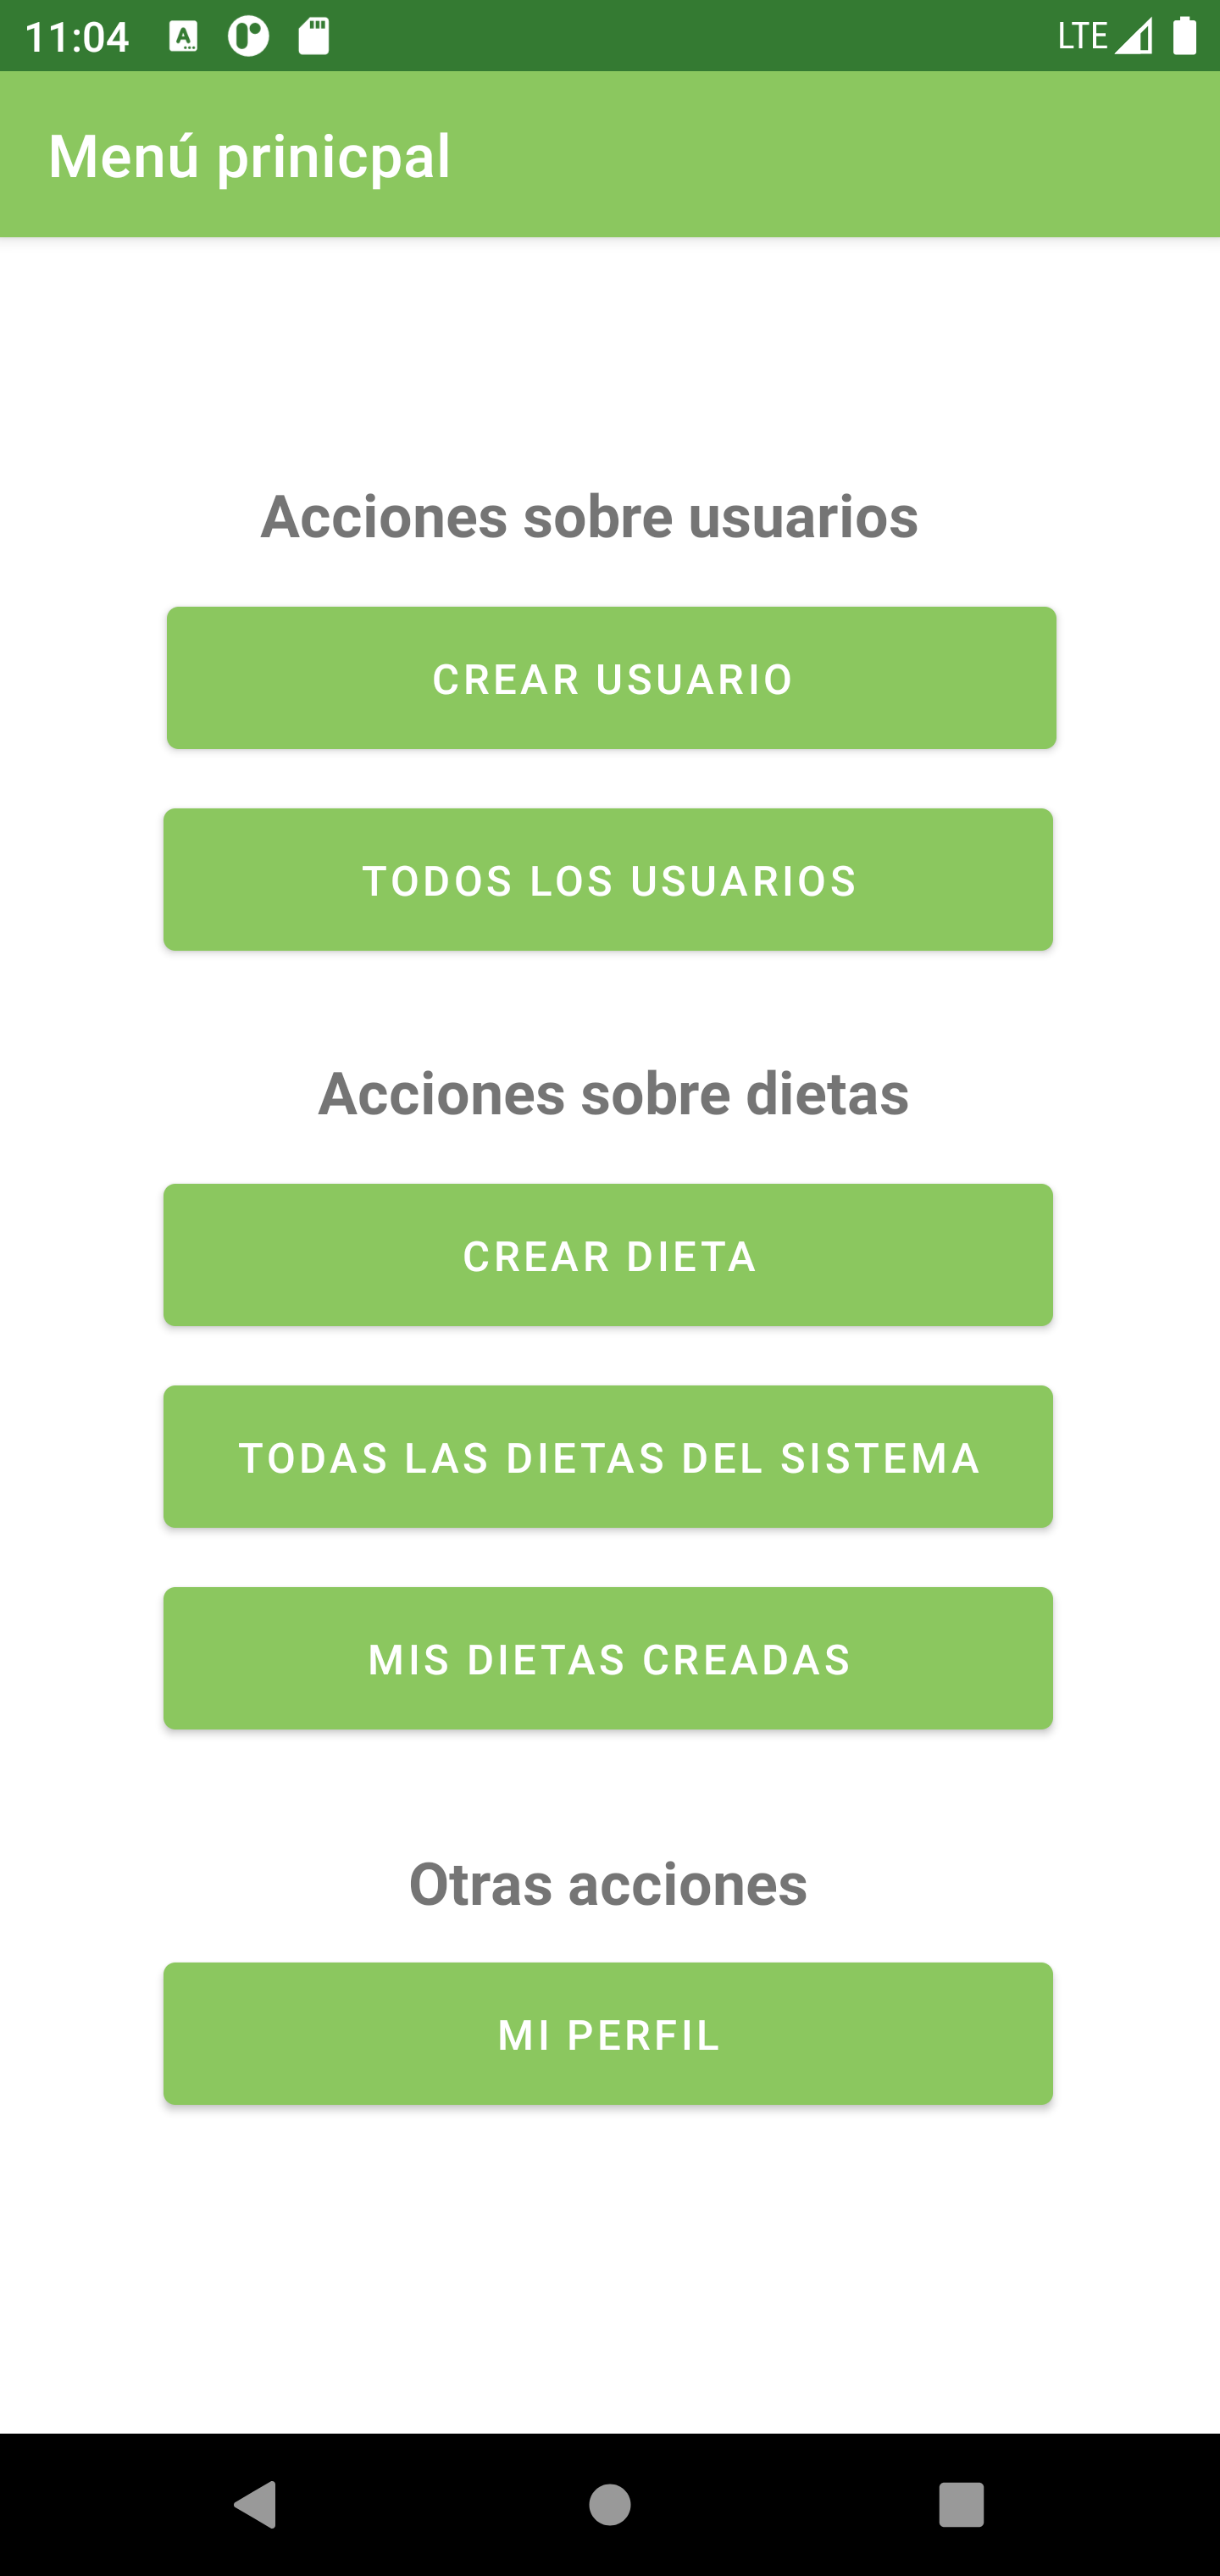
\includegraphics[width=0.4\textwidth]{Images/Annexes/Menu_administradores.png}}
    \caption{Menú principal de la aplicación}
    \label{fig:vista_principal}
\end{figure}


\section{Usuarios}
El grueso de la aplicación tiene este rol, los módulos a los que pueden acceder son todos los de dieta y perfil.
\subsection{Mis dietas creadas} \label{user_my_created_diets}
Si el usuario pulsa mis dietas creadas verá un listado de dietas que ha creado, como se muestra en la figura \ref{fig:mis_dietas}, si no ha creado ninguna o es un nuevo usuario no verá ninguna dieta. En caso de tener dietas el usuario podrá ver el detalle de cada una pulsando en el botón ``Ver dieta``, crear una dieta nueva pulsando el botón con símbolo ``$+$`` ubicado en la esquina inferior derecha o filtrar las dietas con un buscador dinámico que se activa al pulsar la lupa que se encuentra arriba del todo.

\begin{figure}[H]
    \centering
    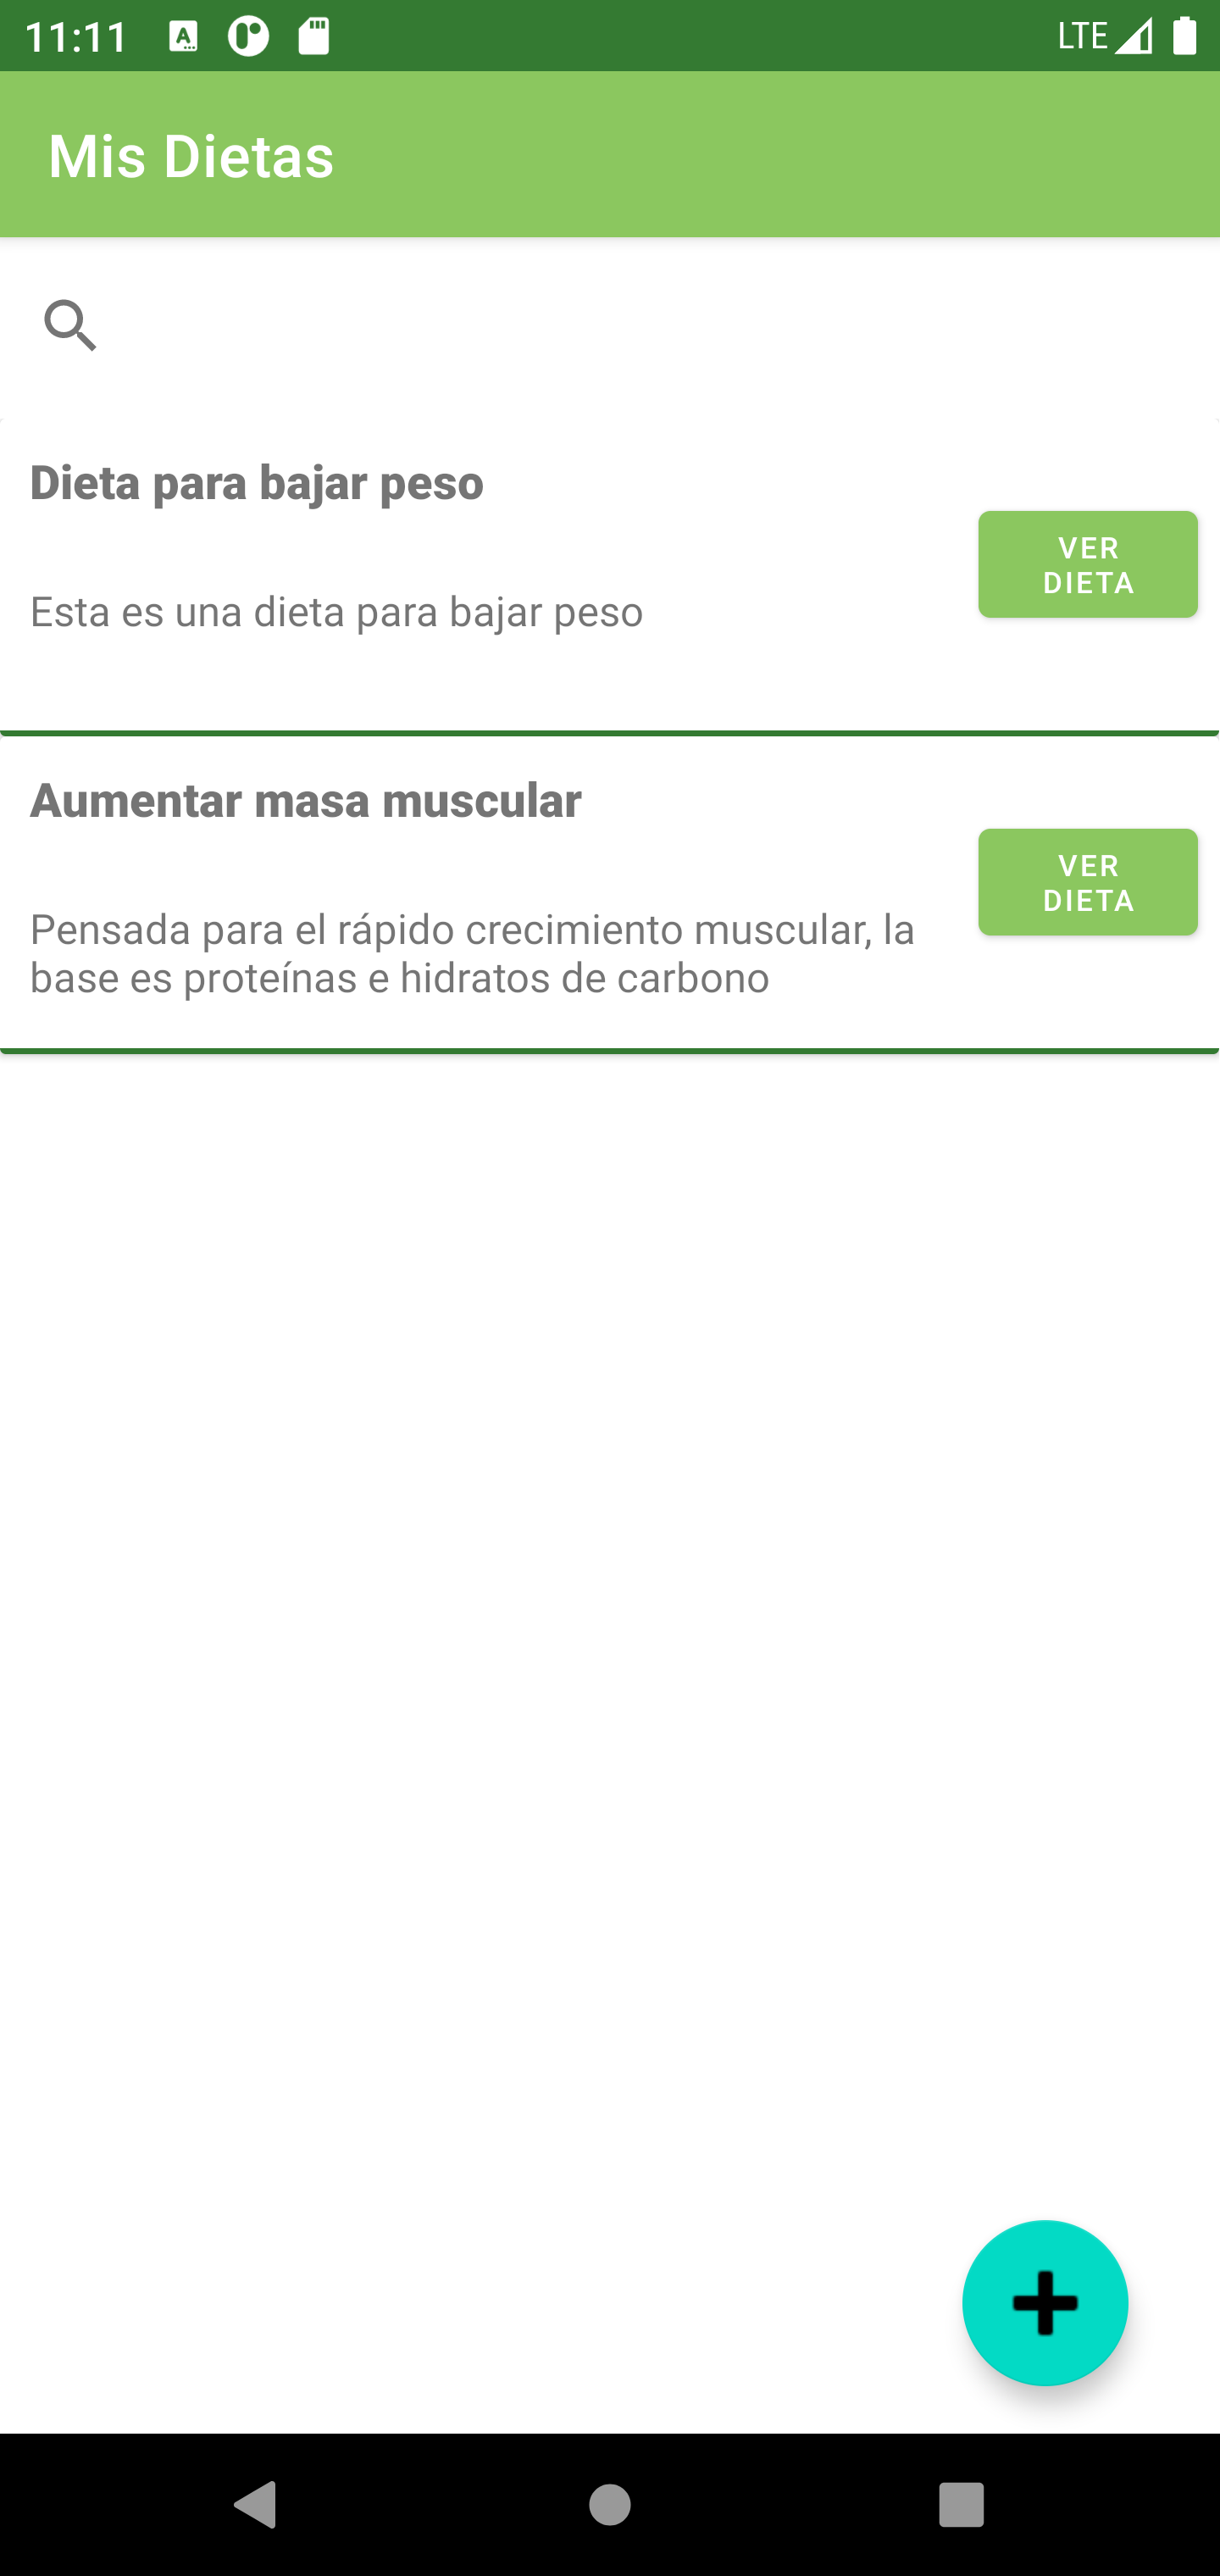
\includegraphics[width=0.5\textwidth]{Images/Annexes/mis_dietas.png}
    \caption{Vista detallada de un documento de una dieta}
    \label{fig:mis_dietas}
\end{figure}

Al presionar “ver dieta” el usuario accede la información detallada de la dieta \ref{fig:mis_dietas_info} y al ser su autor puede editar o eliminar la dieta,  publicarla para el resto de los usuarios o despublicarla si ya estaba publicada. Si la dieta está publicada aparecerá la opción de acceder a los comentarios de la dieta.
\begin{figure}[H]
    \centering
    \subfigure{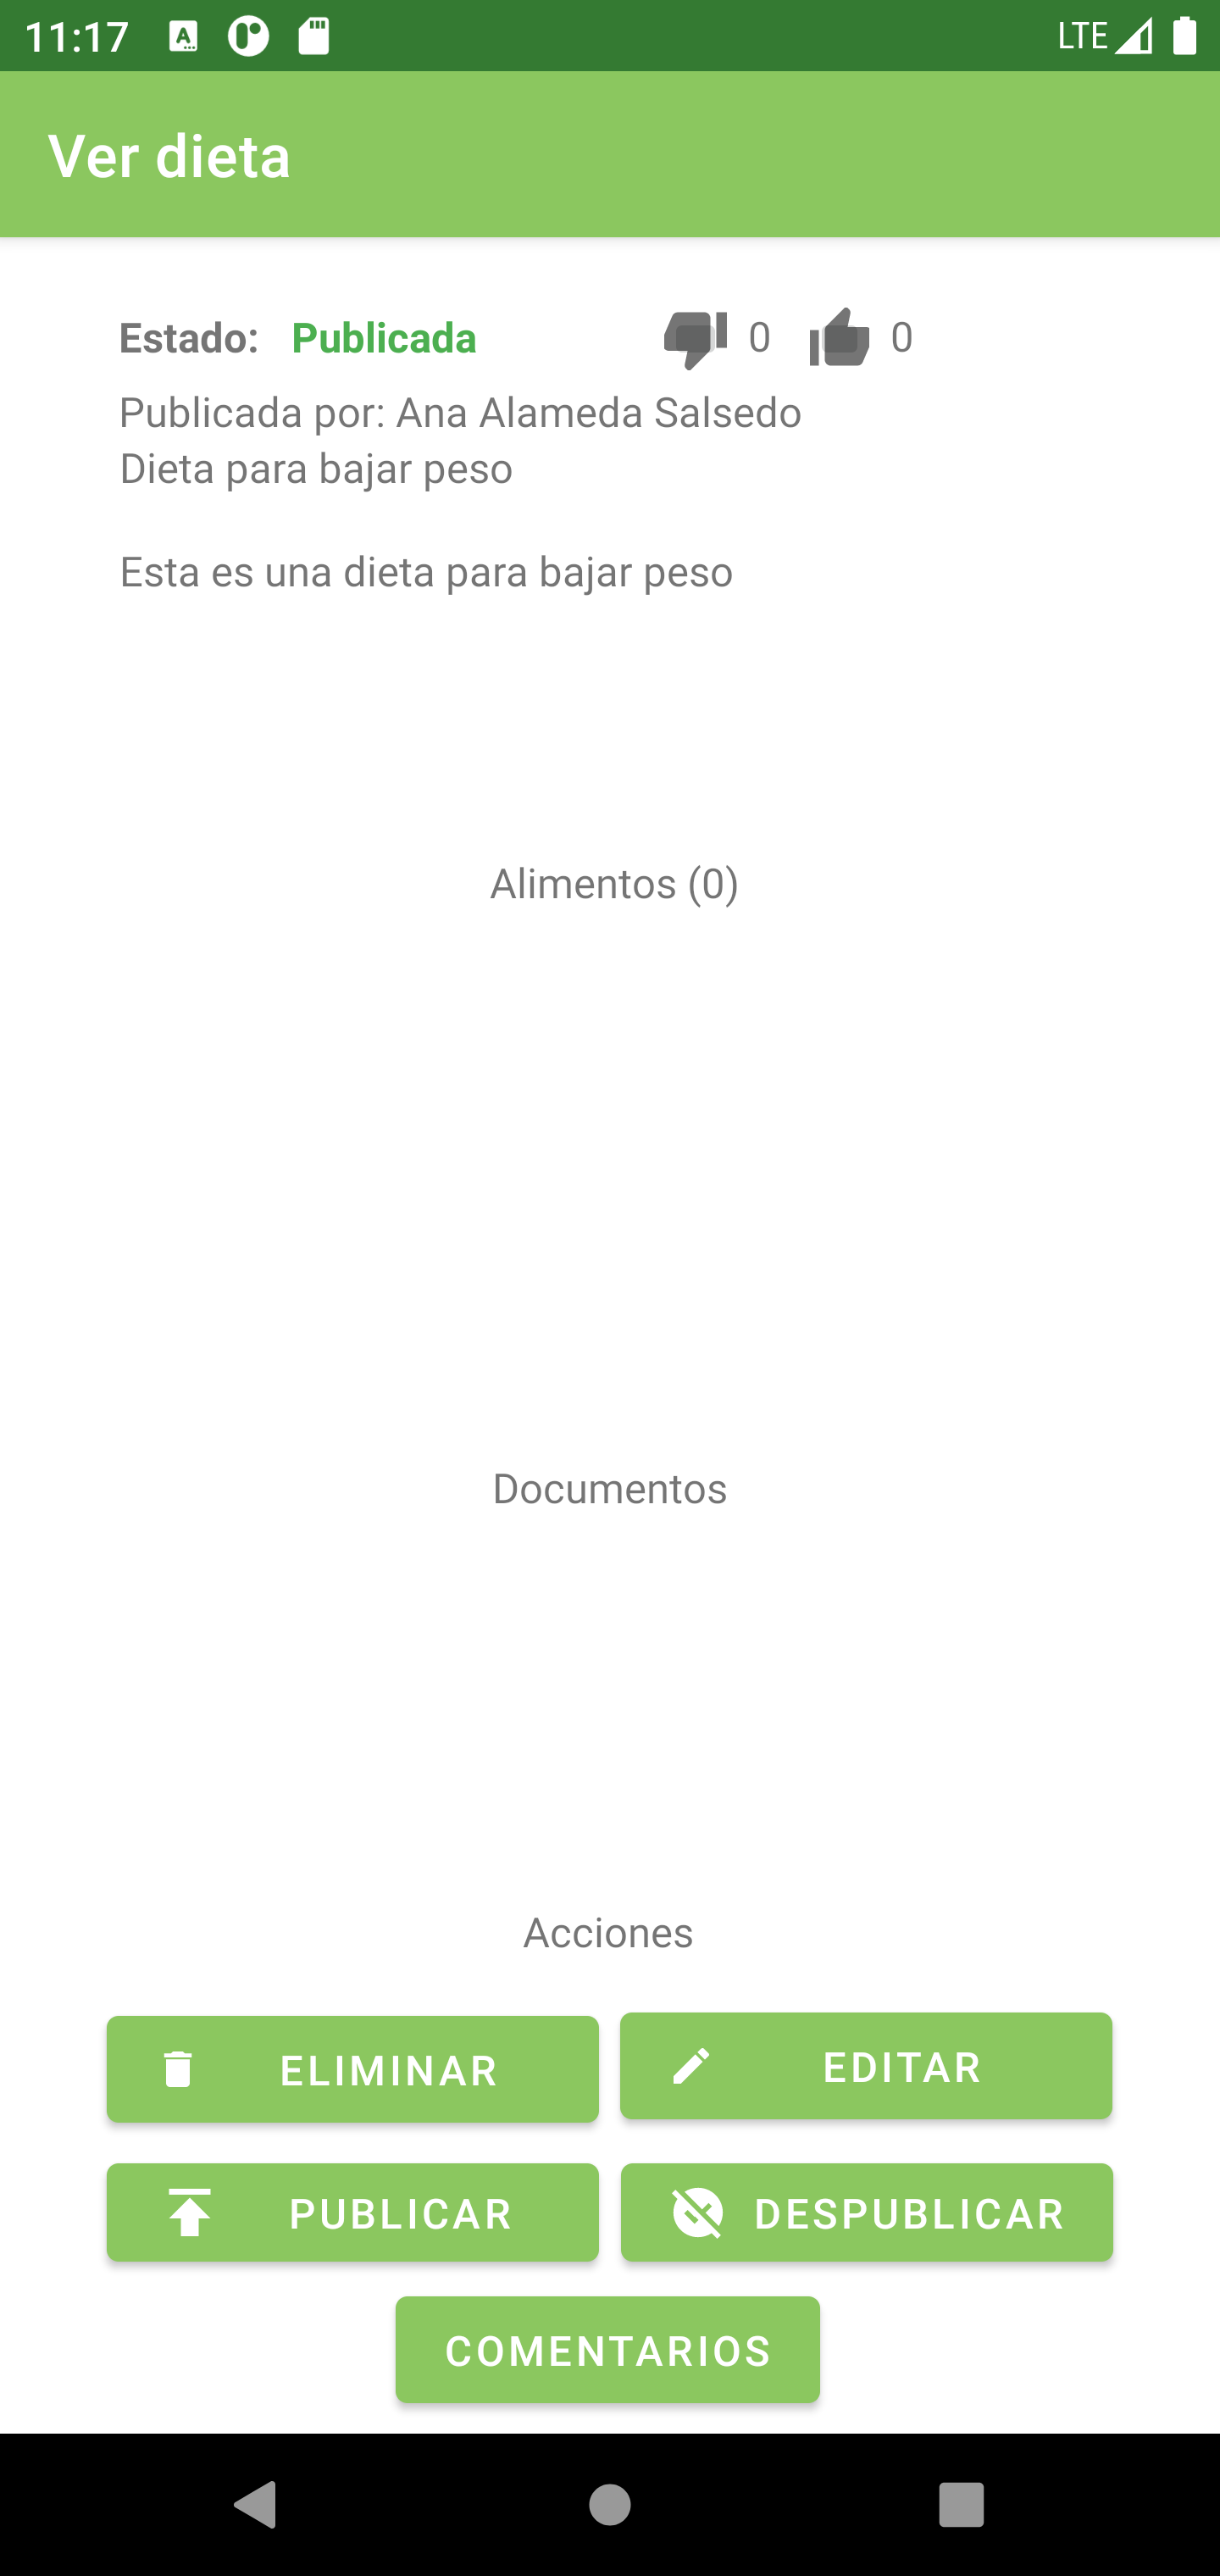
\includegraphics[width=0.4\textwidth]{Images/Annexes/ver_dieta_publicada.png}}
    \subfigure{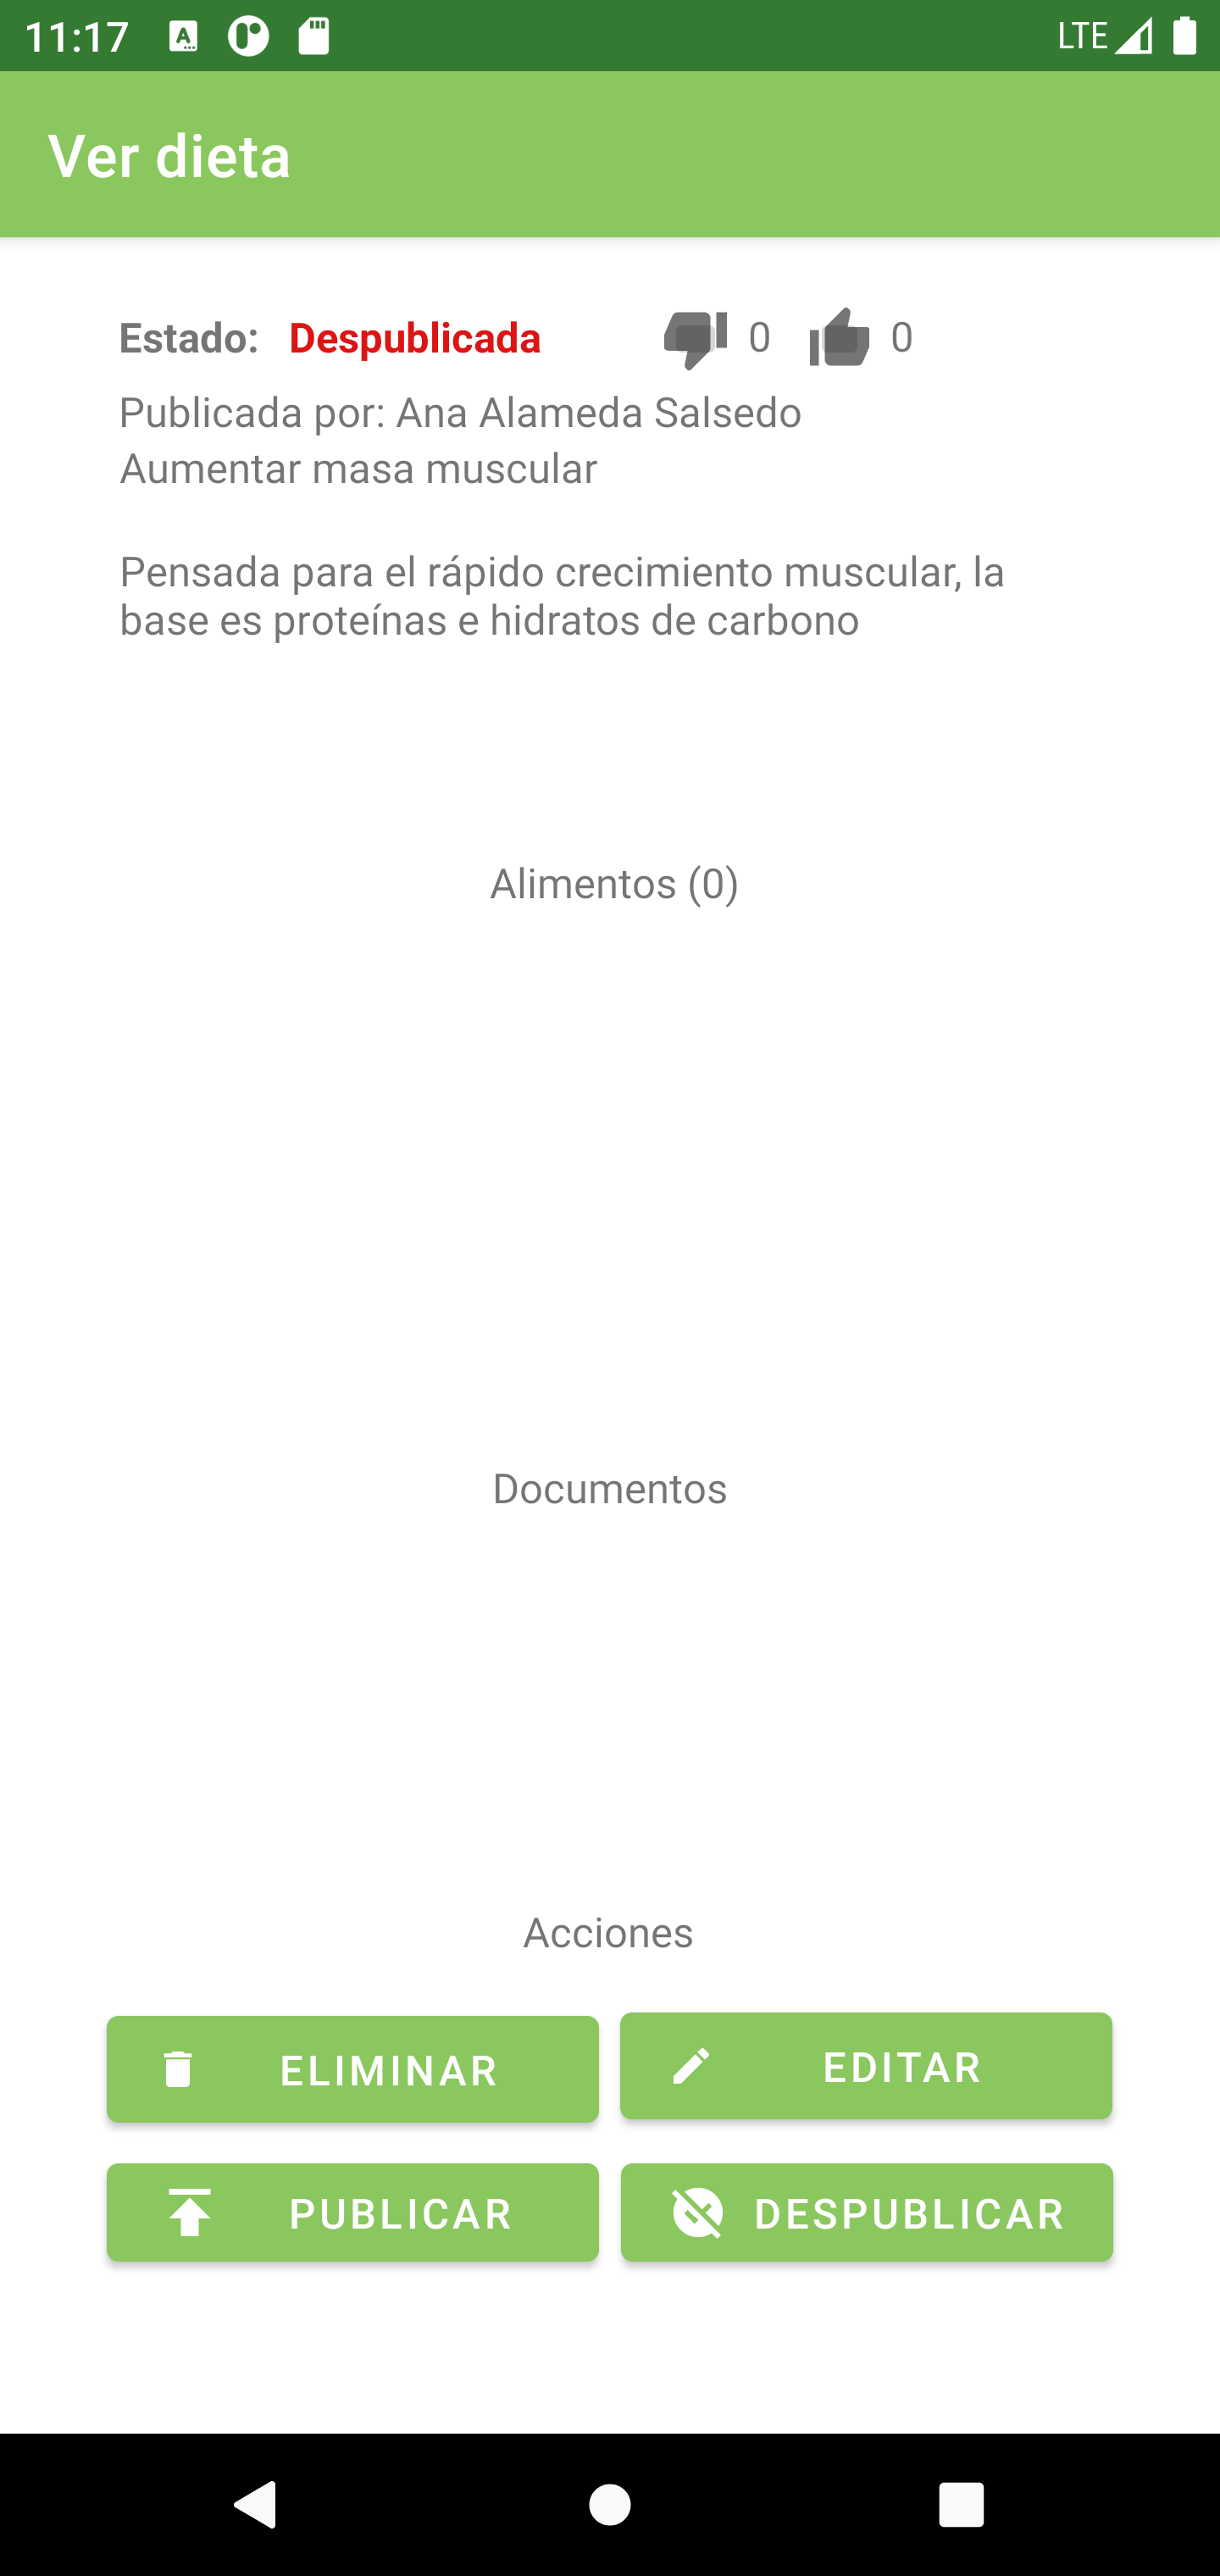
\includegraphics[width=0.4\textwidth]{Images/Annexes/ver_dieta_despublicada.png}}
    \caption{Una dieta publicada y despublicada}
    \label{fig:mis_dietas_info}
\end{figure}

Si el usuario presiona editar podrá añadir alimentos a la dieta y/o subir documentos en formato PDF con información que el usuario considere necesaria para la dieta como por ejemplo aportar estudios que la respalden.

Para añadir un alimento el usuario dispone de varias formas, como se muestra en la figura \ref{fig:añadir_alimentos} , desde la cámara, en cuyo caso deberá escanear el código de barras del alimento o manualmente ya sea escribiendo el código de barras o escribiendo los datos del alimento campo por campo.
\begin{figure}[H]
    \centering
    \subfigure[Añadir manualmente]{\includegraphics[width=0.4\textwidth]{Images/Annexes/añadir_alimentos.png}}
    \subfigure[Añadir con cámara]{\includegraphics[width=0.4\textwidth]{Images/Annexes/añadir_alimentos_camara.jpg}}
    \caption{Vista de añadir alimentos a una dieta}
    \label{fig:añadir_alimentos}
\end{figure}


\subsection{Dietas publicadas}
Cuando el usuario accede a las dietas publicadas \ref{fig:dietas_publicadas} podrá visualizar todas las dietas que los usuarios de DietNow han creado y publicado para que estén al alcance de todos, el usuario dispondrá de un buscador dinámico en la parte de arriba para poder filtrar rápidamente las dietas por palabras clave. 

Para cada dieta publicada podrá visualizar el número de ``Me gusta`` que tiene y el número de visualizaciones y al presionar el botón ``ver dieta`` podrá visualizar el contenido de la dieta además de empezar a seguirla presionando el botón con forma de estrella o abrir la sección de comentarios para leer los comentarios y/o dejar el suyo propio.
\begin{figure}[H]
    \centering
    \subfigure[Todas las dietas publicadas]{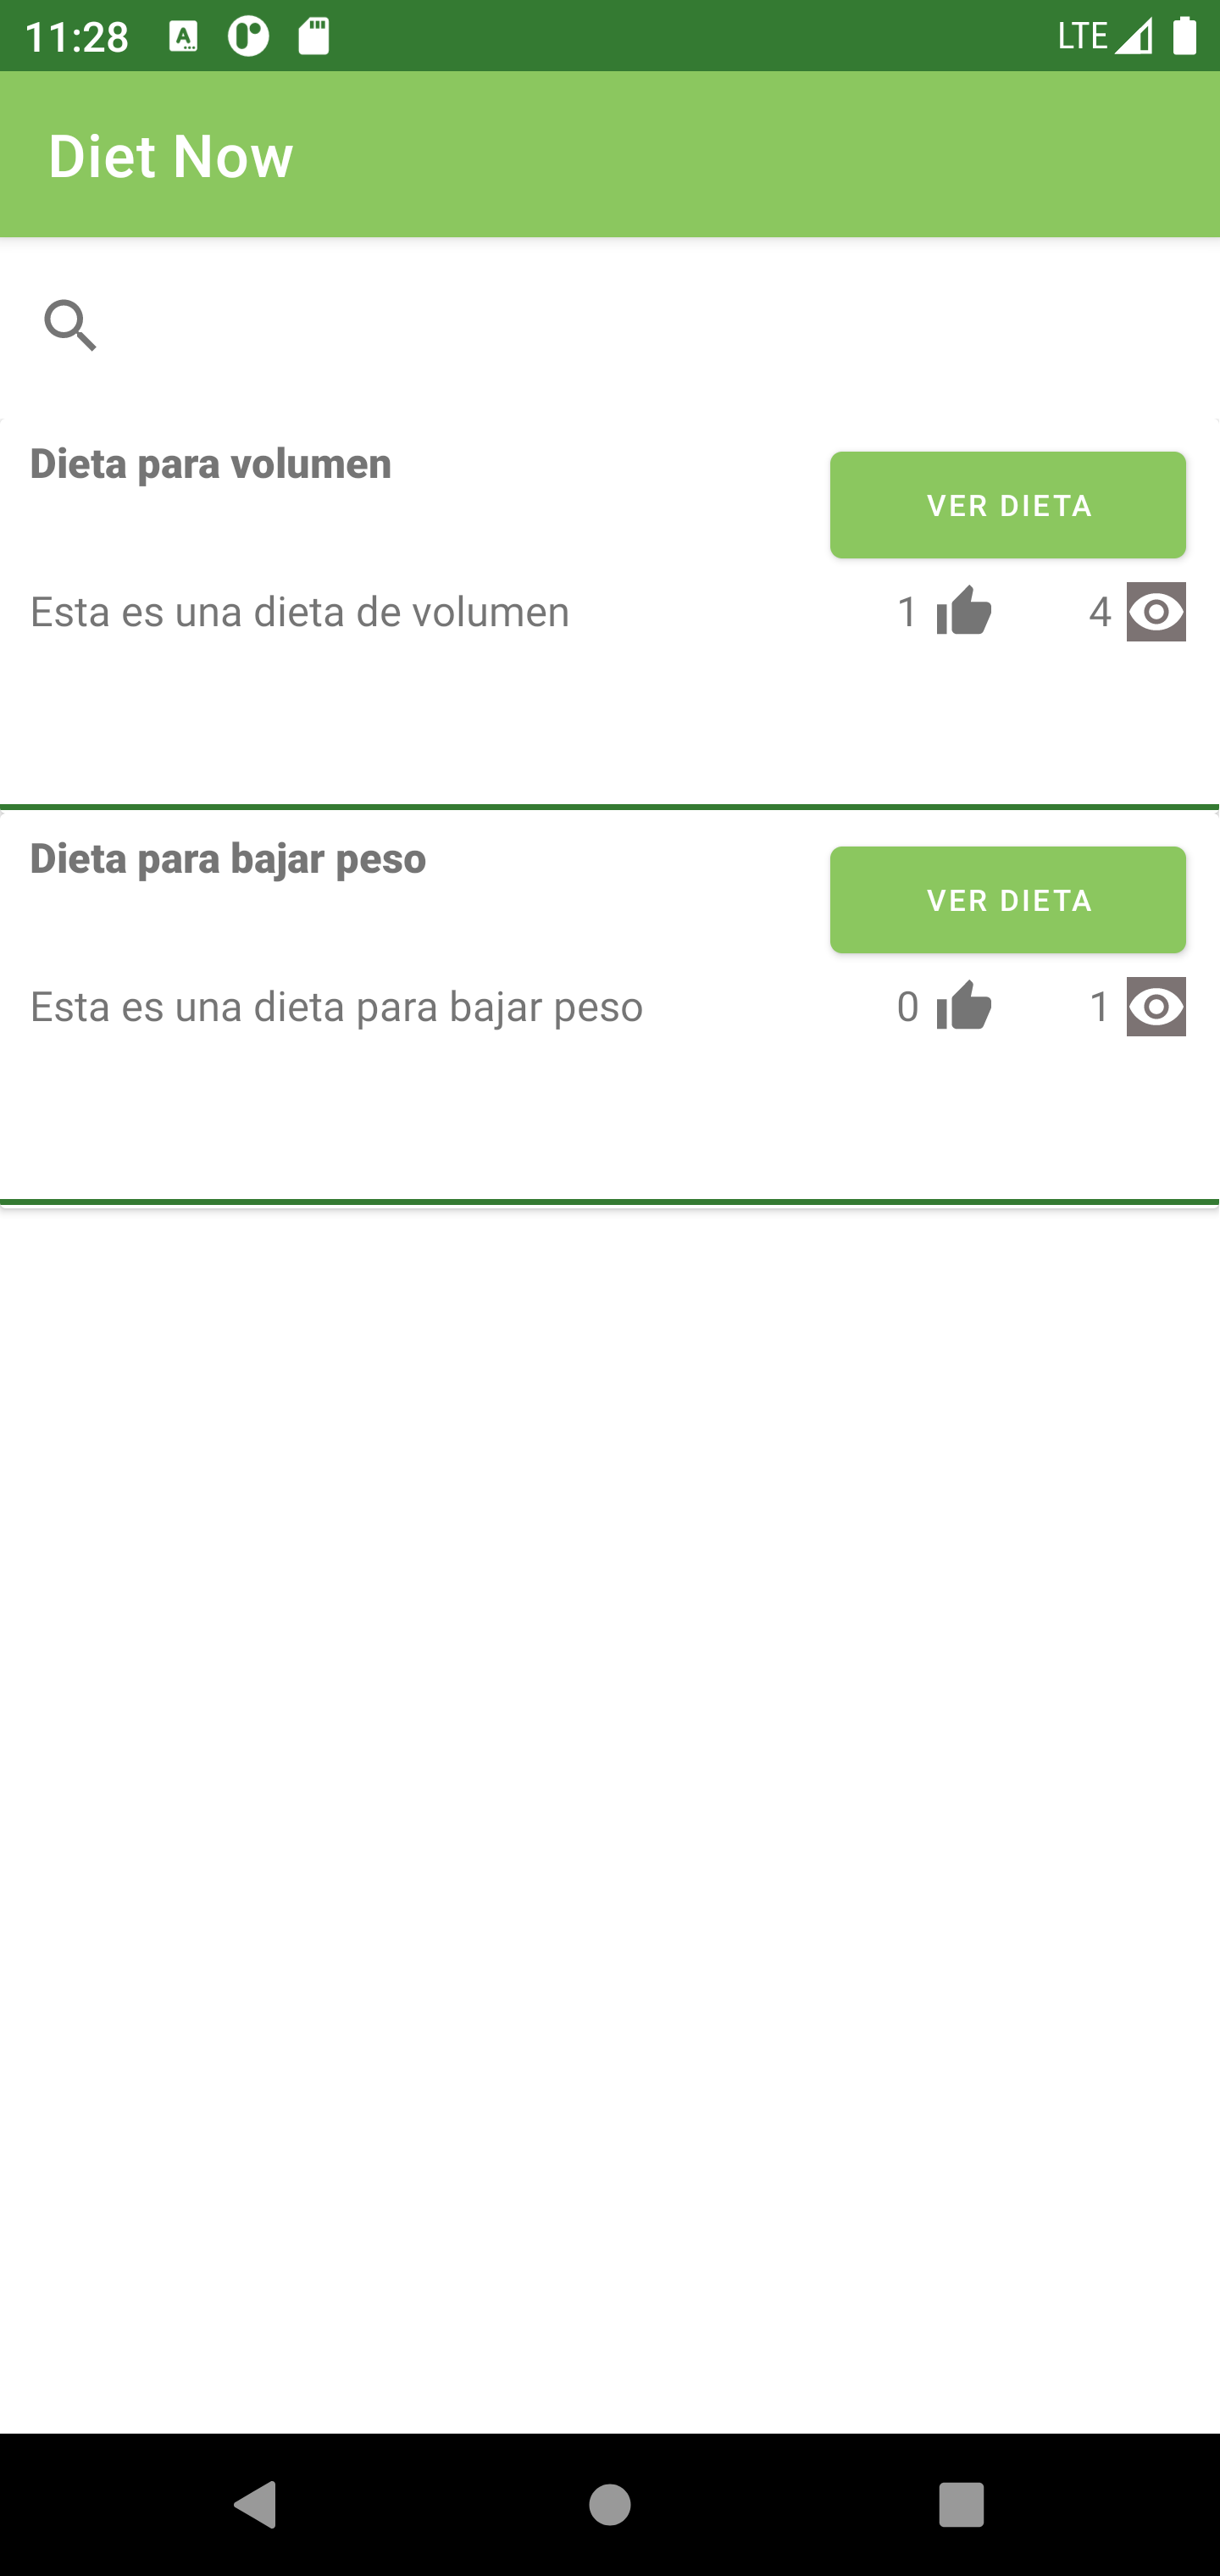
\includegraphics[width=0.4\textwidth]{Images/Annexes/vista_dietas_publicadas.png}}
    \subfigure[Vista detallada de dieta]{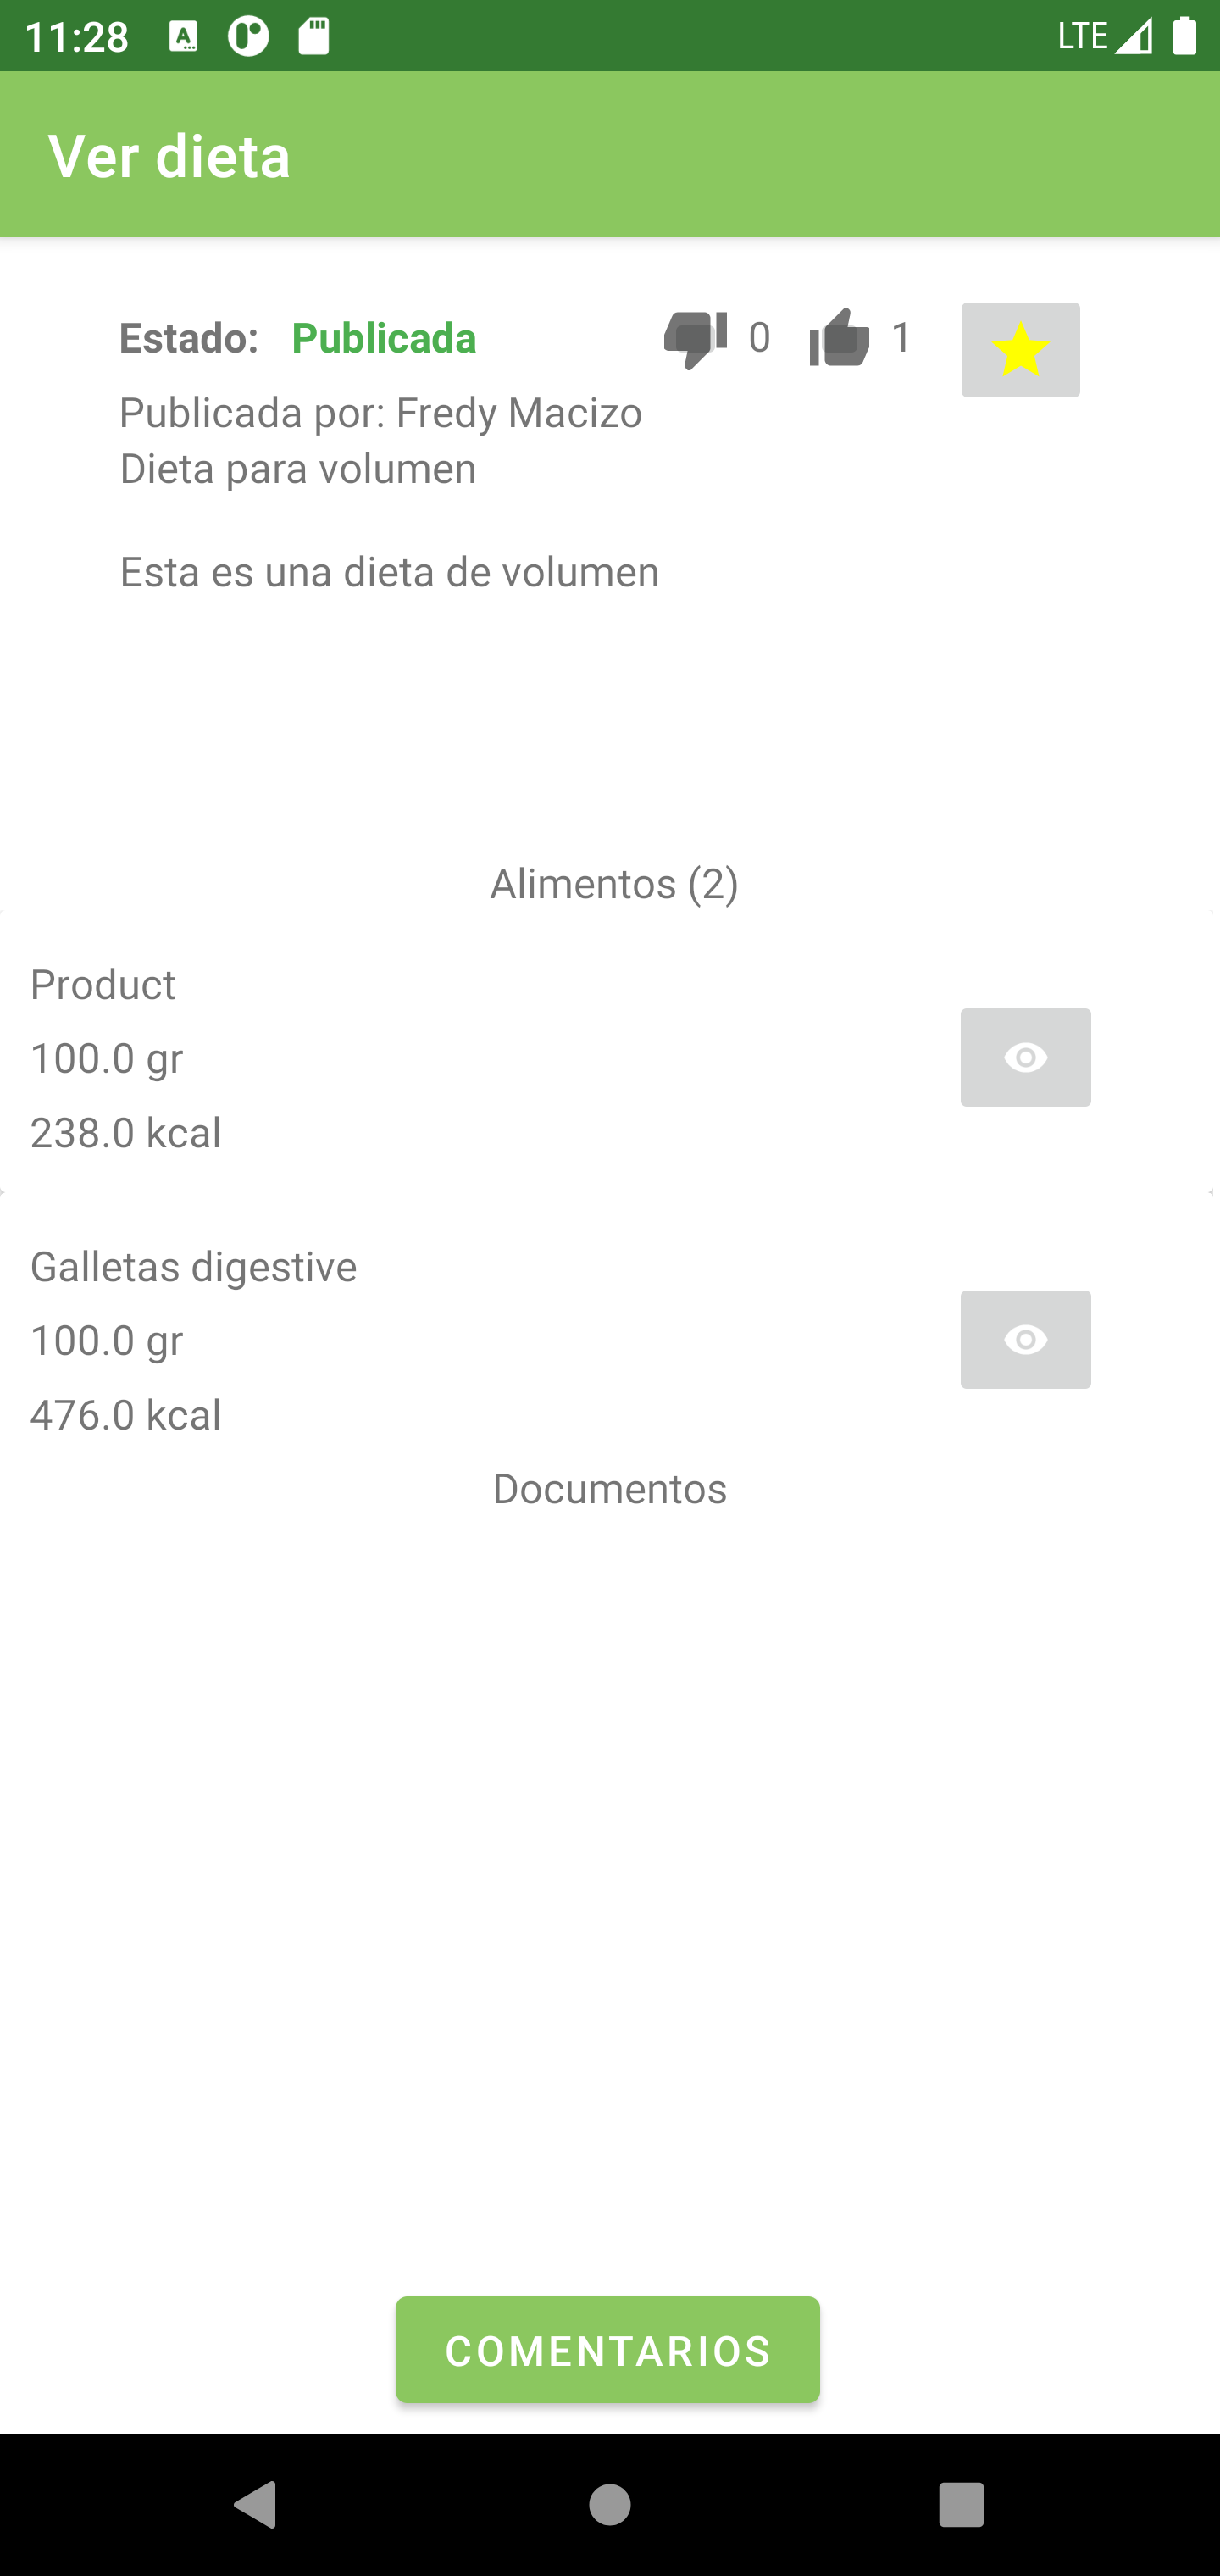
\includegraphics[width=0.4\textwidth]{Images/Annexes/vista_dieta_publicada_seguida.png}}
    % \subfigure[Vista de los comentarios de la dietas seguida]{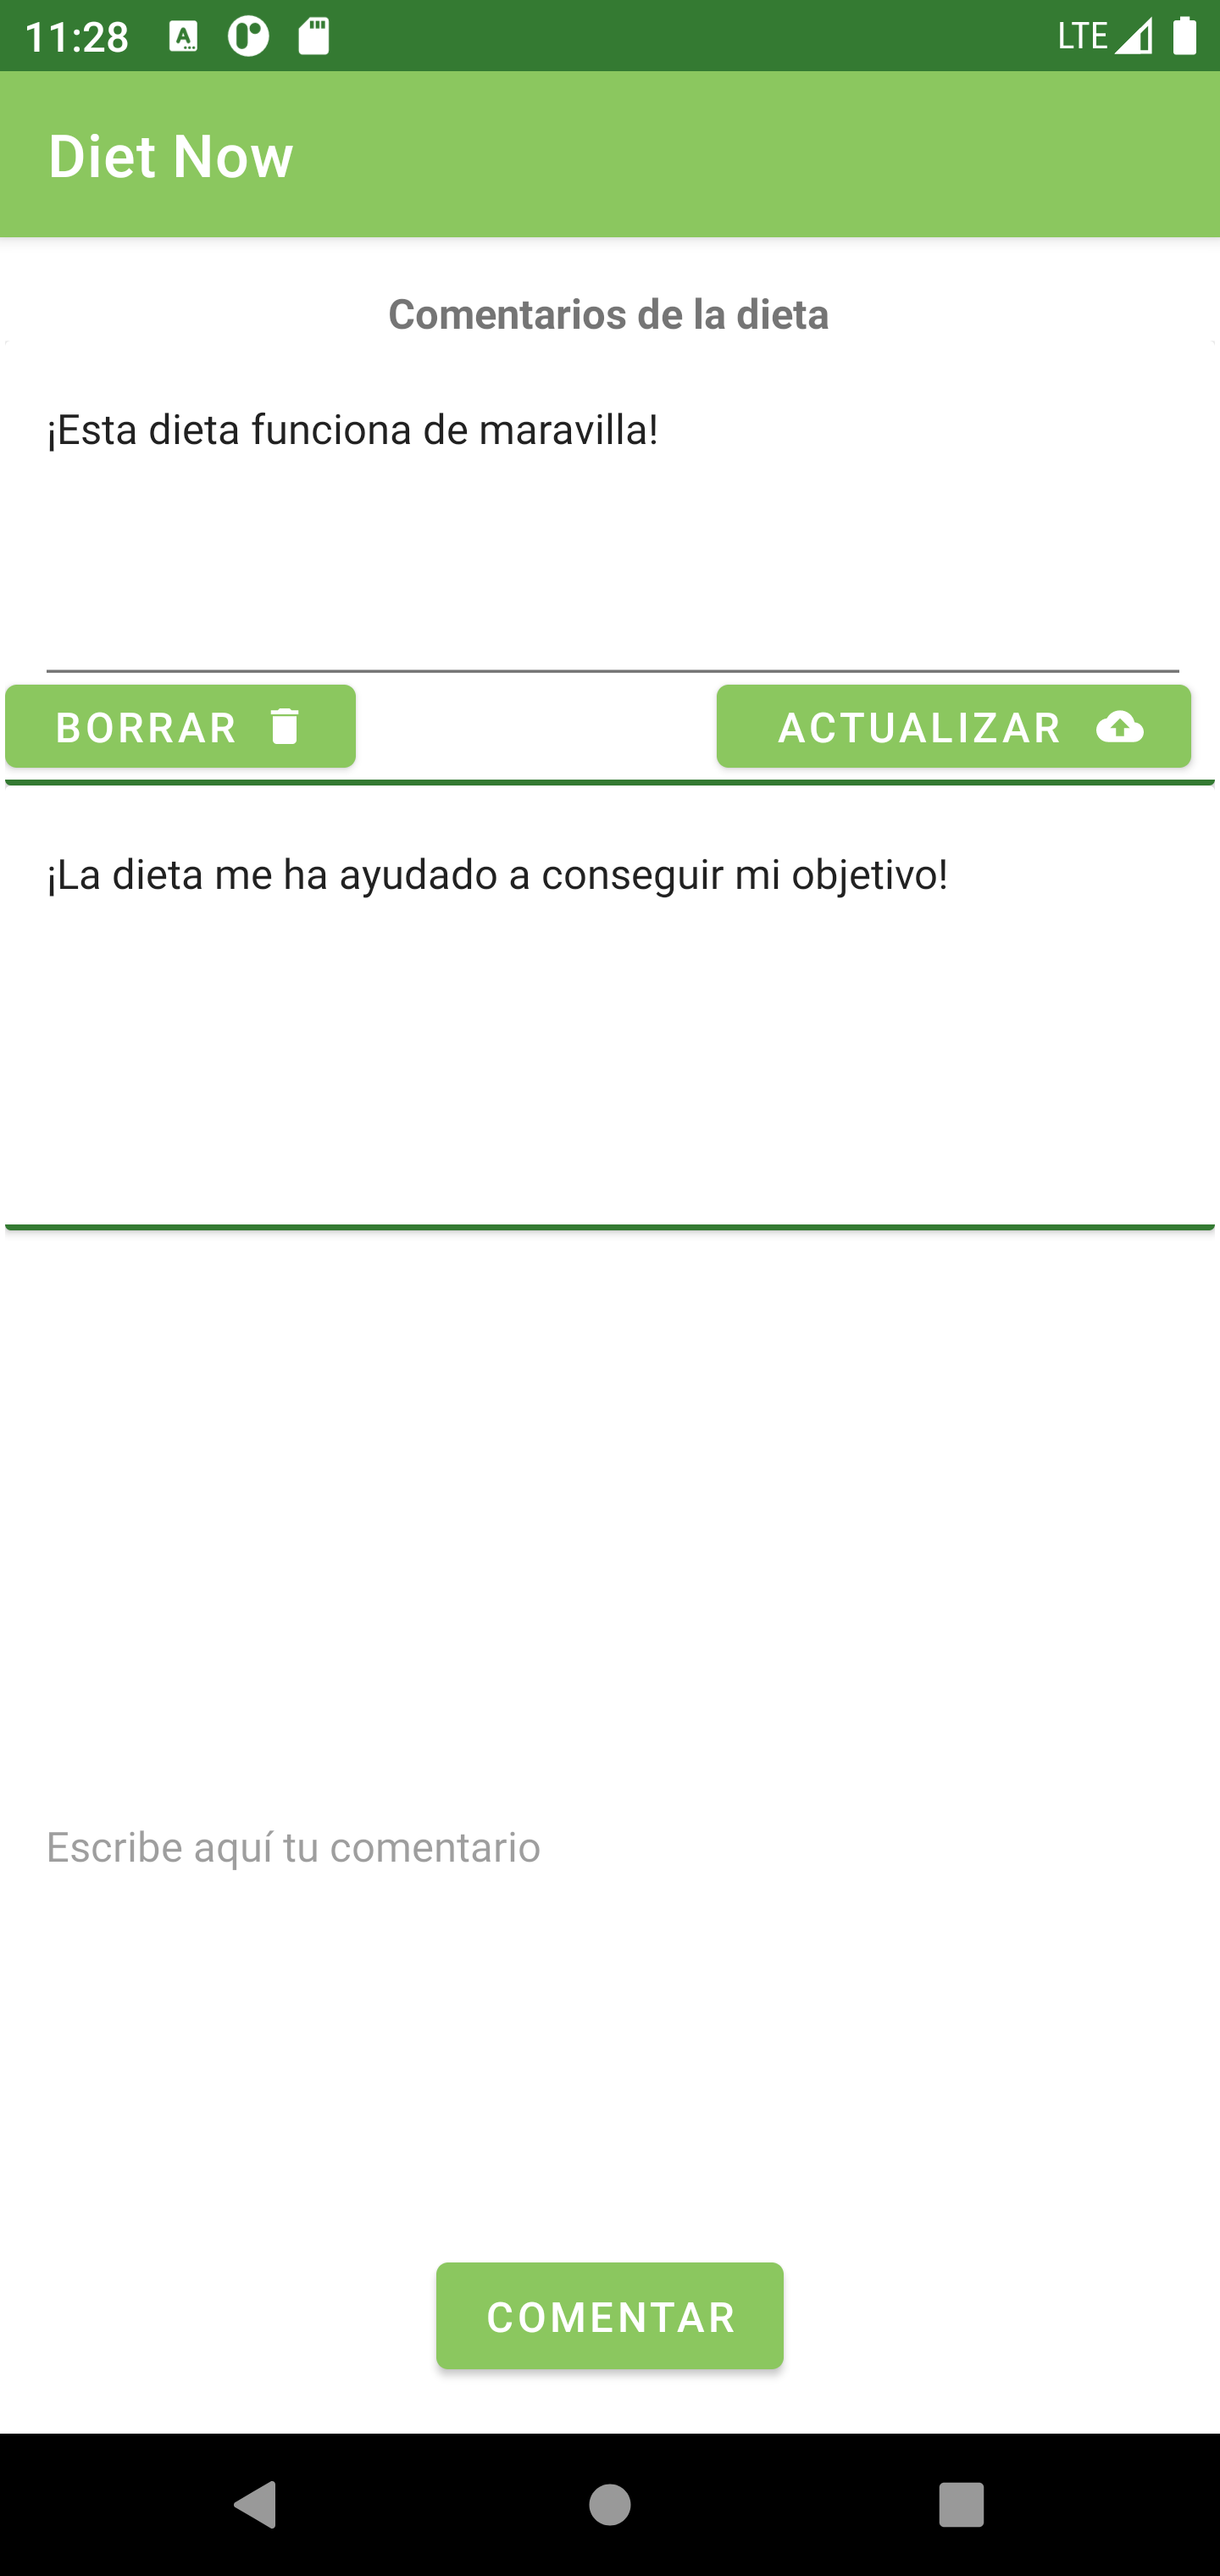
\includegraphics[width=0.3\textwidth]{Images/Annexes/vista_comentarios_dieta_seguida.png}}
    \caption{Vista dietas publicadas}
    \label{fig:dietas_publicadas}
\end{figure}


\subsection{Dieta seguida}
Si el usuario pulsa esta opción verá la dieta que está siguiendo, como se muestra en la figura \ref{fig:dieta_seguida}, y podrá registrar los alimentos y la cantidad que ha comido en el día actual, podrá ver lo que ingirió a lo largo de la semana y dejar su feedback sobre la dieta ya sea dejando un me gusta, un no me gusta o un comentario, también podrá dejar de seguir la dieta.

\begin{figure}[H]
    \centering
    \subfigure{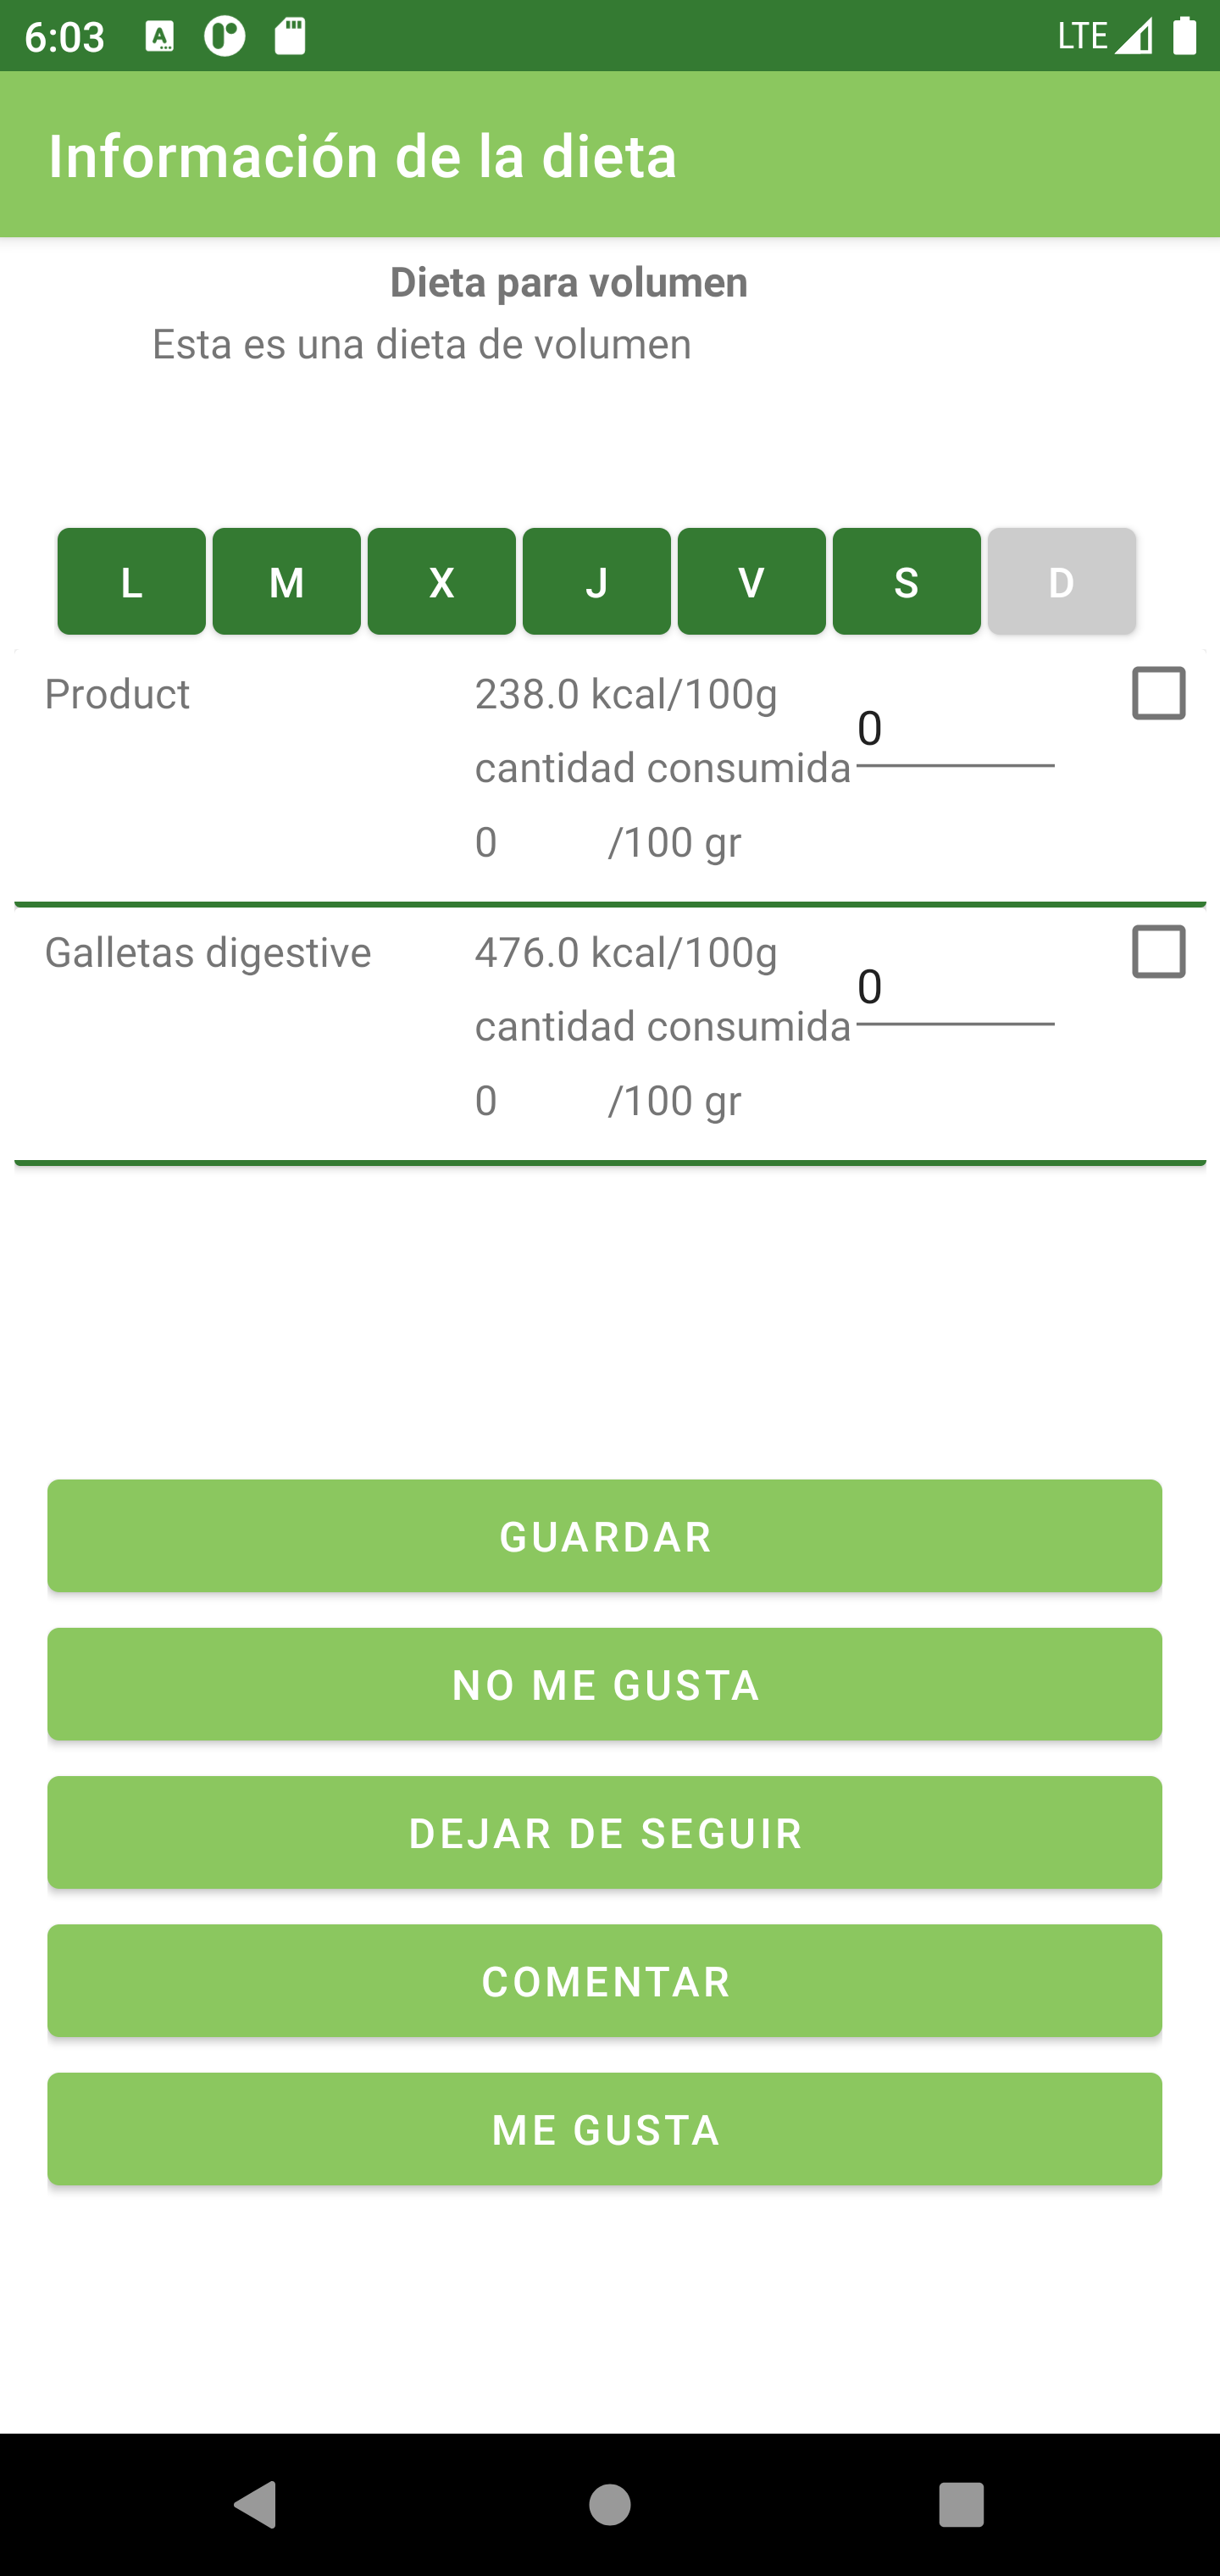
\includegraphics[width=0.4\textwidth]{Images/Annexes/dieta_seguida1.png}}
    \subfigure{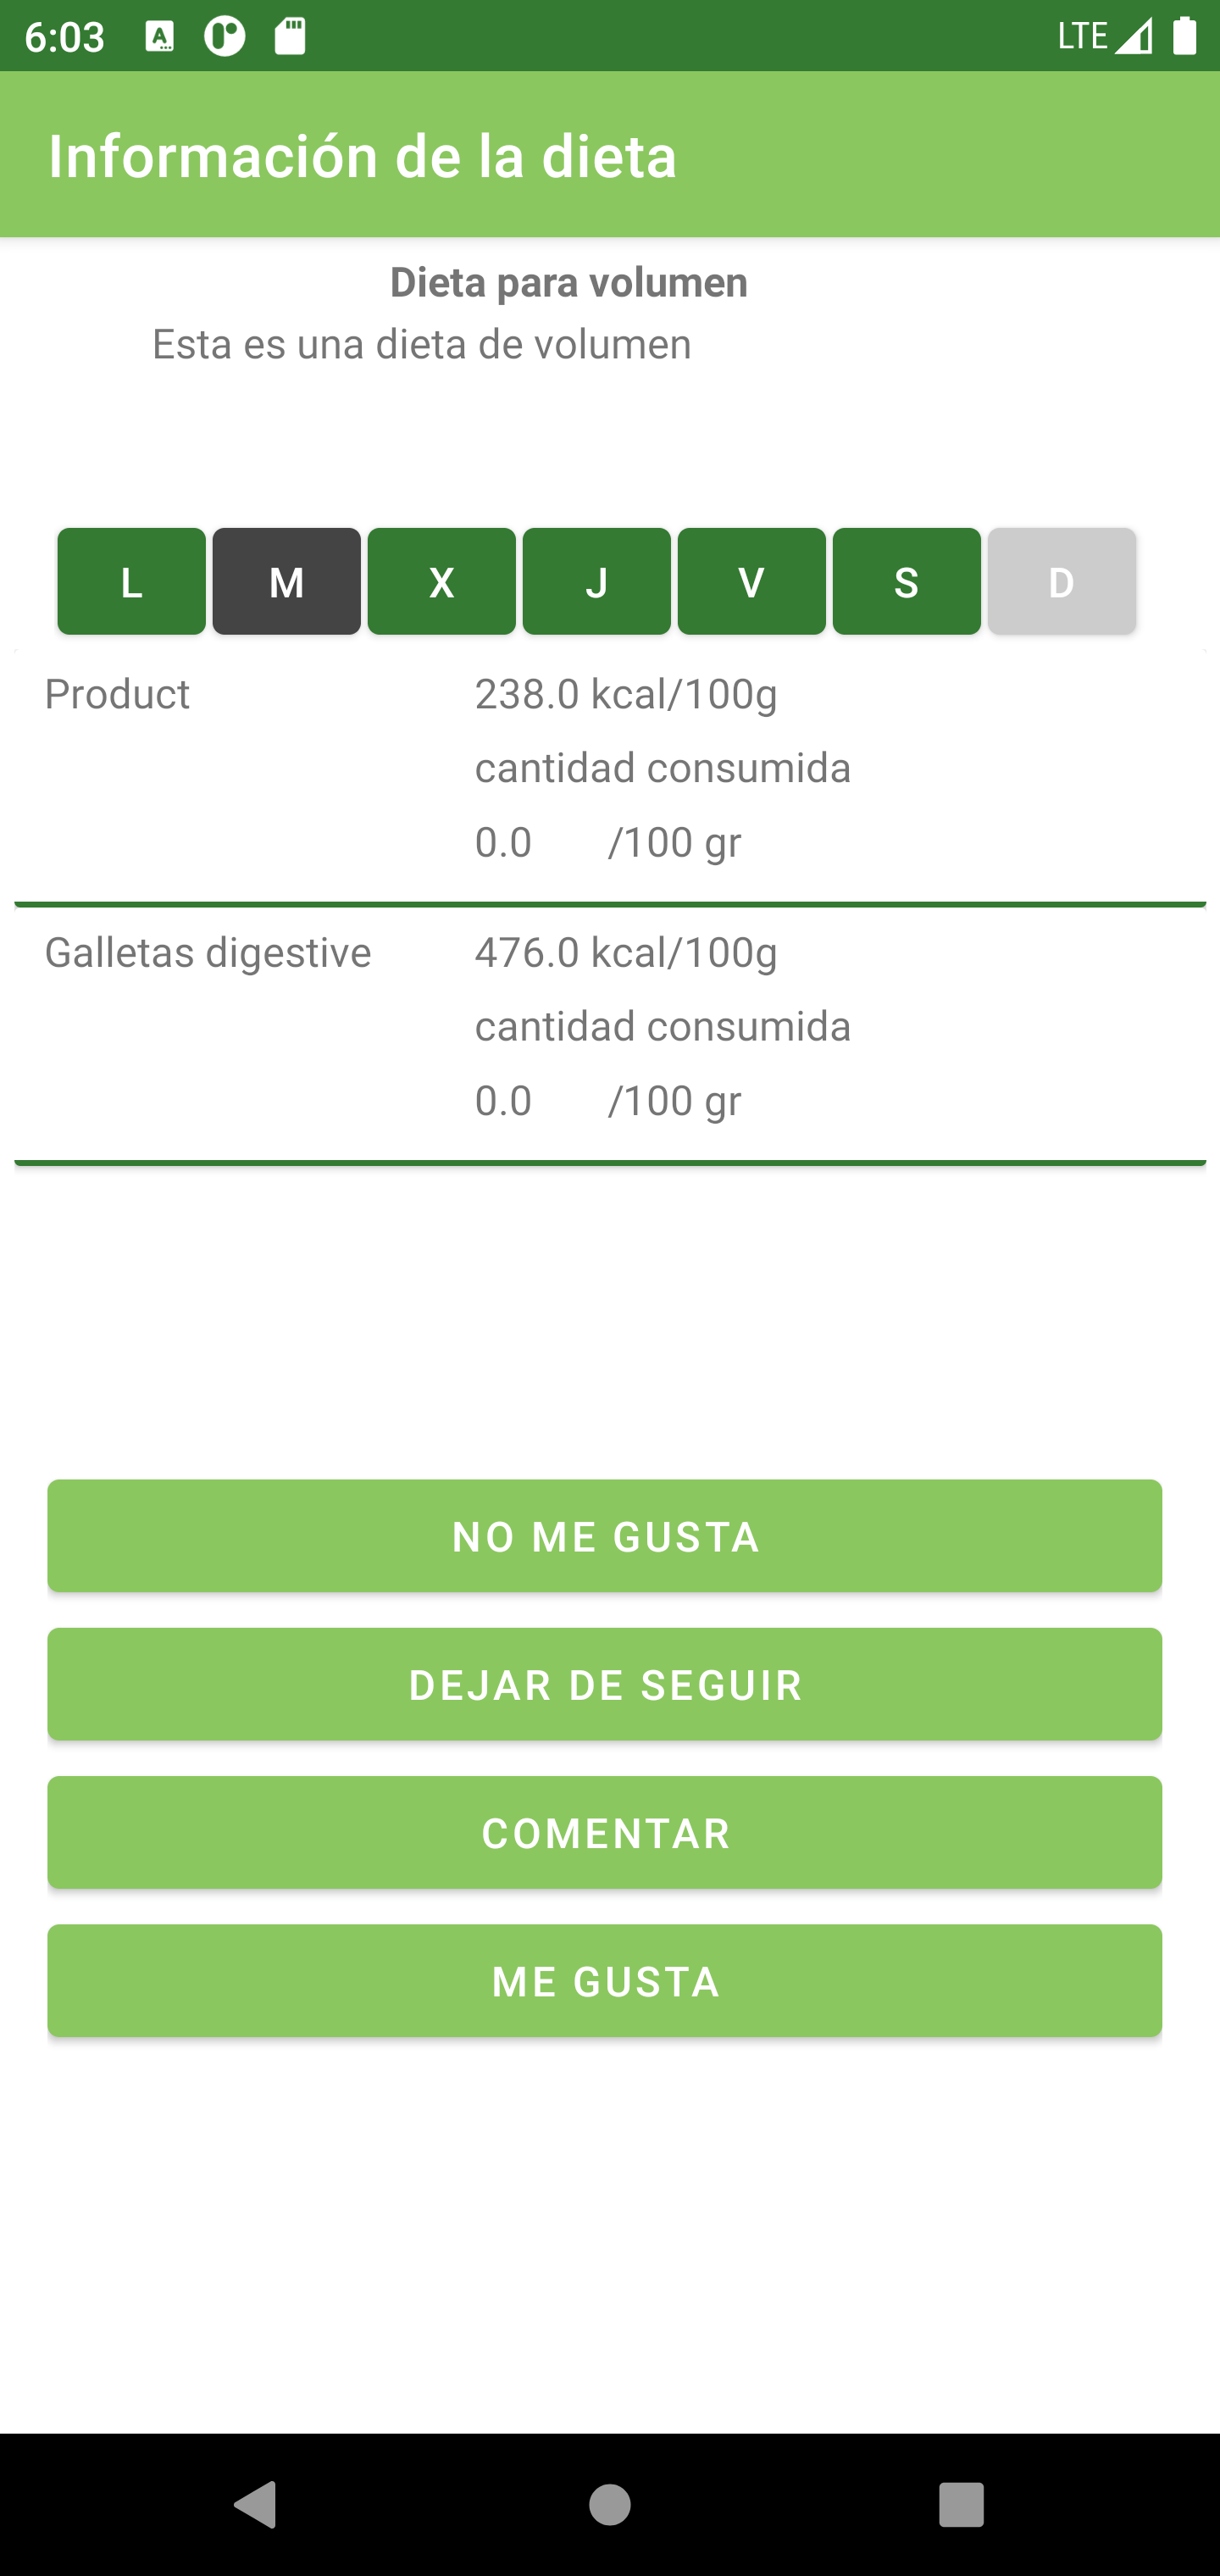
\includegraphics[width=0.4\textwidth]{Images/Annexes/dieta_seguida2.png}}
    \caption{Vista de dieta seguida}
    \label{fig:dieta_seguida}
\end{figure}

\subsection{Ver perfil}
Si se selecciona esta opción, el usuario será redirigido a una ventana que mostrará su información personal y las gráficas asociadas a él, como se puede apreciar en la Figura \ref{fig:user_profile}. Las acciones que puede realizar en esta vista son registrar pasos y/o peso del día actual, ver el historial de dietas seguidas, actualizar sus datos personales, cambiar la imagen de perfil, eliminar el perfil y cerrar sesión.

\begin{figure}[H]
    \centering
    \subfigure{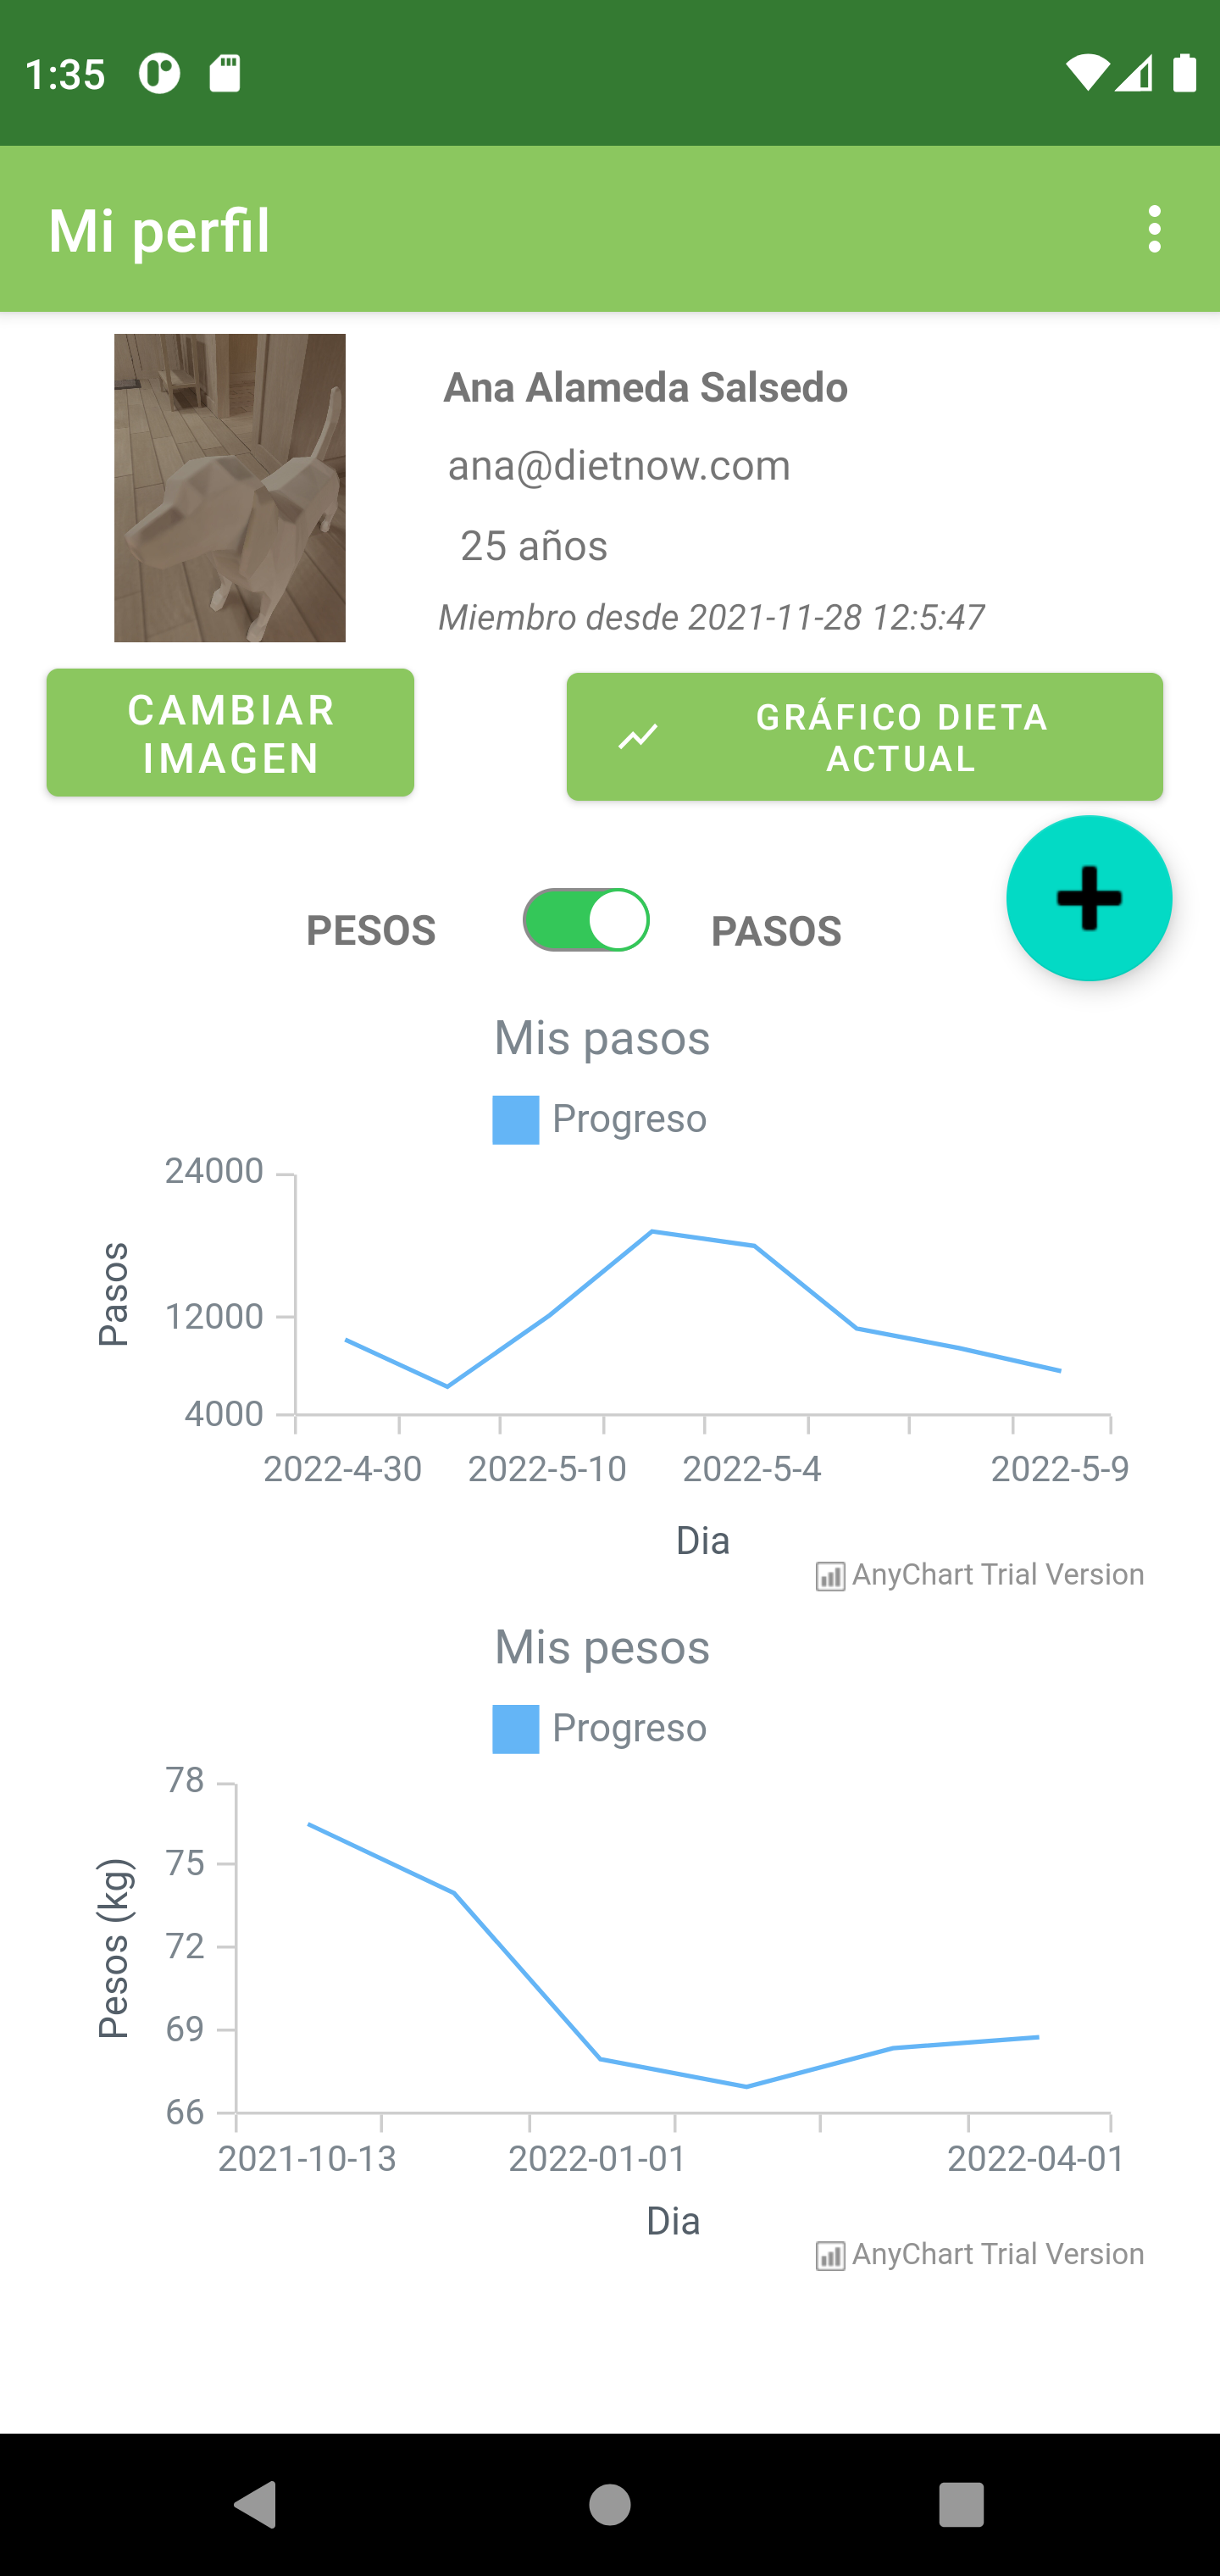
\includegraphics[width=0.4\textwidth]{Images/Annexes/userProfile.png}}
    \subfigure{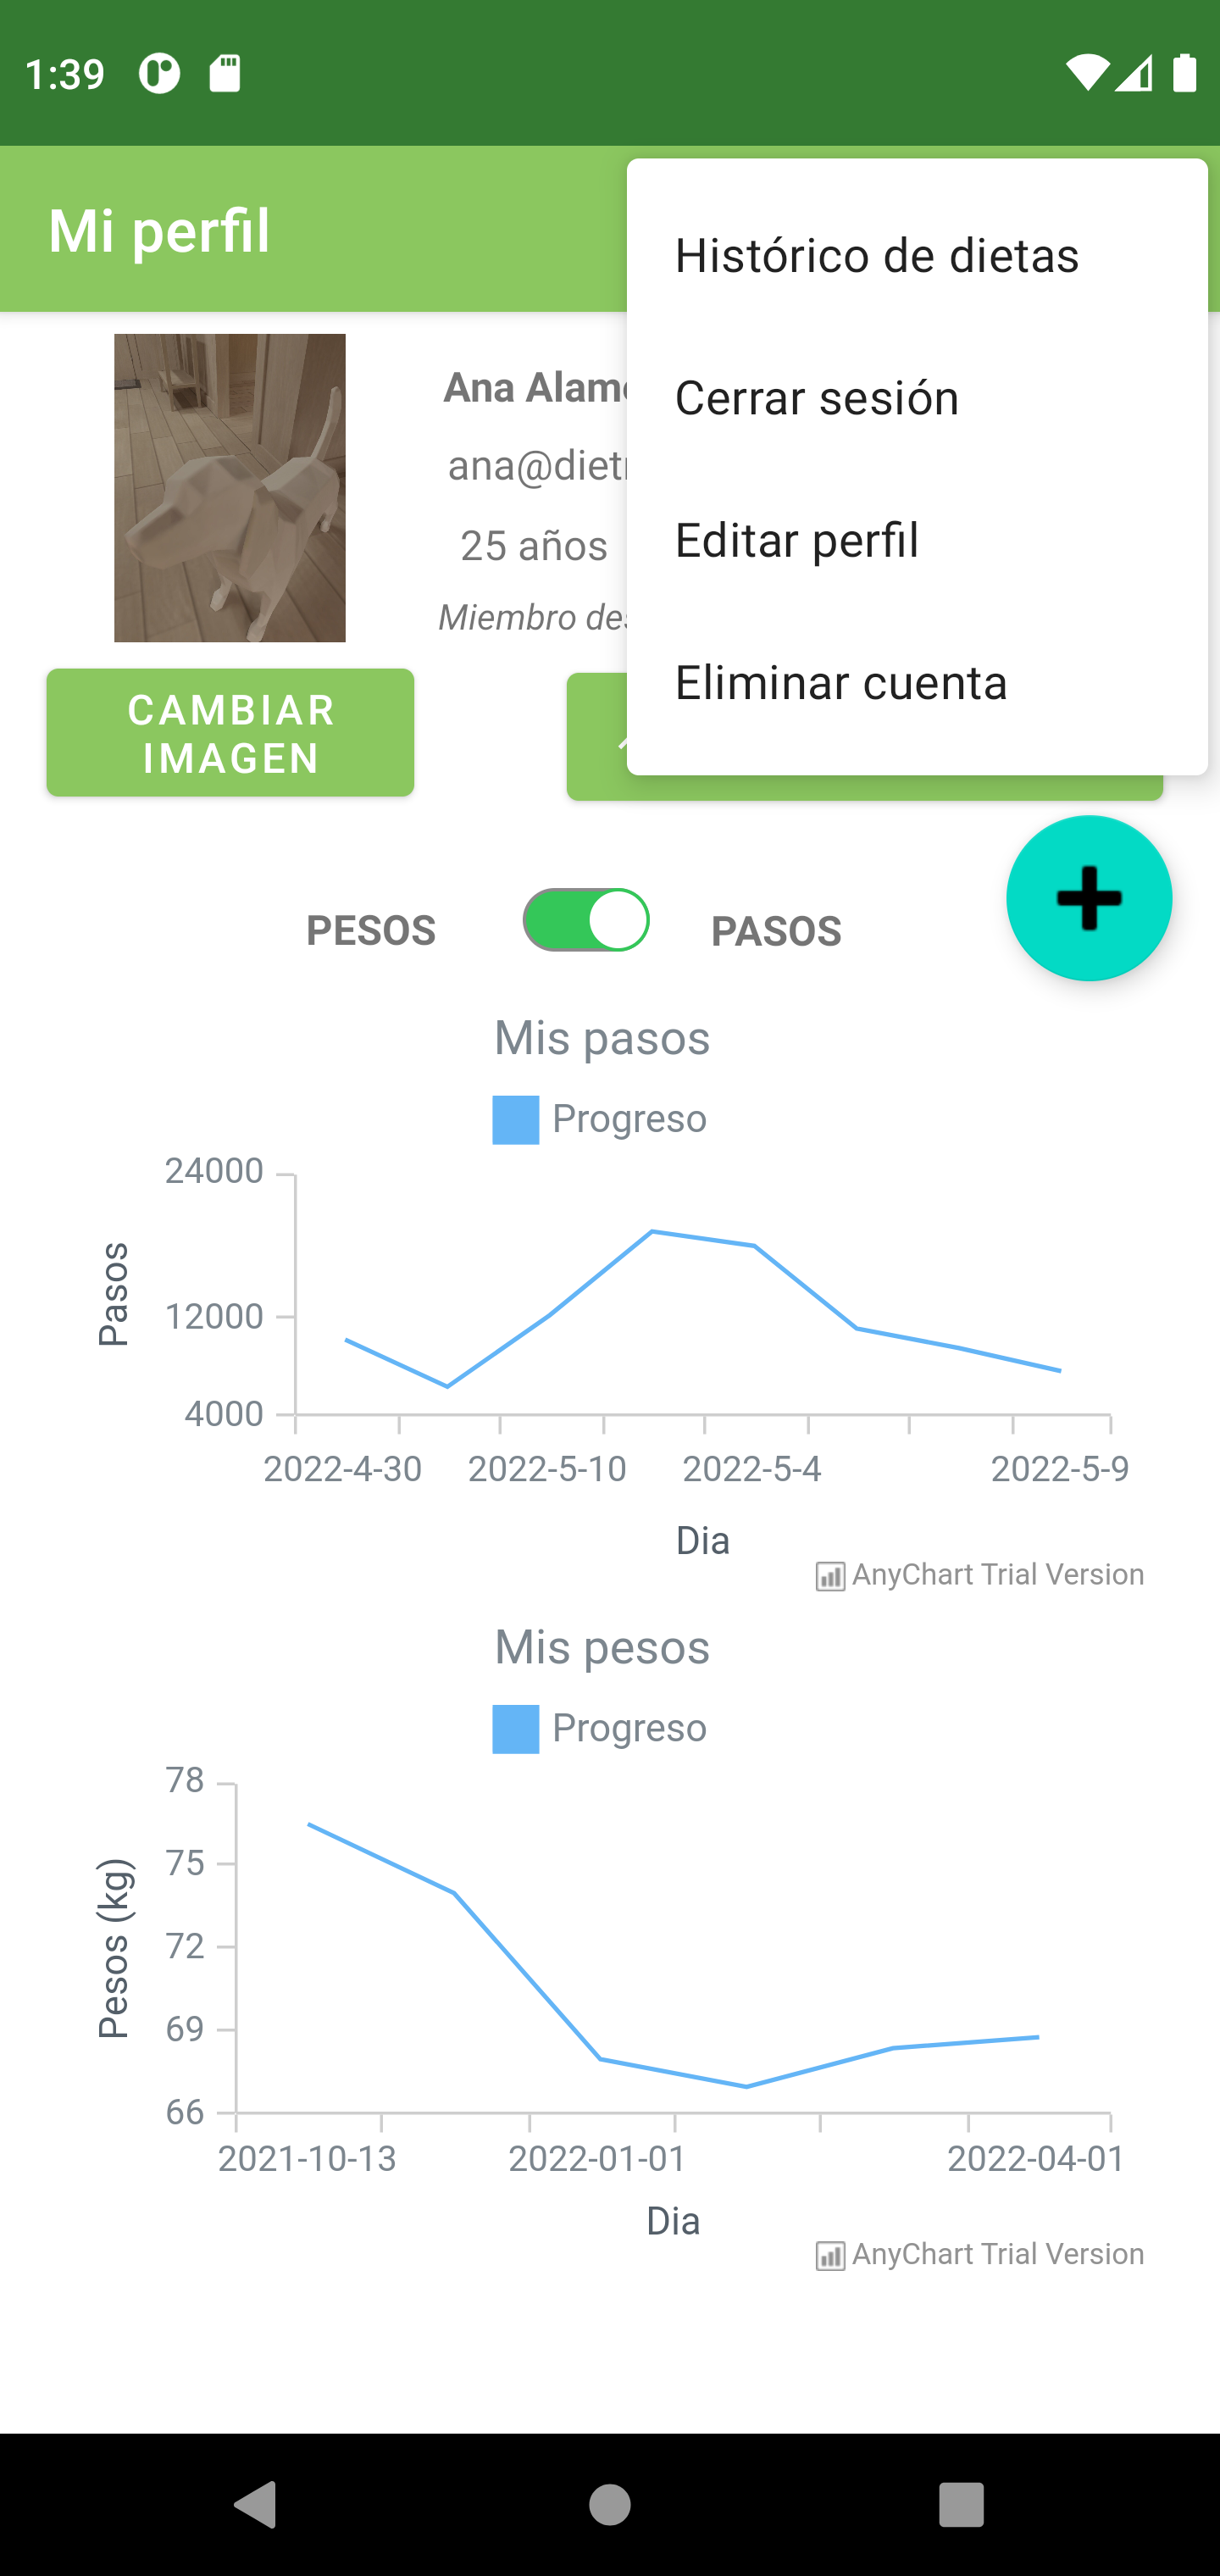
\includegraphics[width=0.4\textwidth]{Images/Annexes/userProfile2.png}}
    \caption{Vista del perfil de usuario}
    \label{fig:user_profile}
\end{figure}

%%%%%%%%%%%%%%%%%%%%%%%%%%%%%%%%%%%%%%%%%%%%%%%%%%%%%%%%%%%%

\section{Administradores}
Rol pensado para asegurar el correcto funcionamiento de la aplicación, algunas de las funciones de este rol son la gestión de usuarios, creación de dietas predeterminadas y control de contenido.

\subsection{Crear usuario}
Mediante esta opción se accede a un formulario similar al de registro de usuario, como se muestra en la figura \ref{fig:crear_usuario_admin}, donde el administrador puede crear una cuenta, la diferencia respecto al formulario de registro es que mientras que en el formulario de registro la cuenta creada siempre tendrá rol usuario, en crear cuenta el administrador puede decidir el rol de la cuenta que está creando.

\begin{figure}[H]
    \centering
    \subfigure{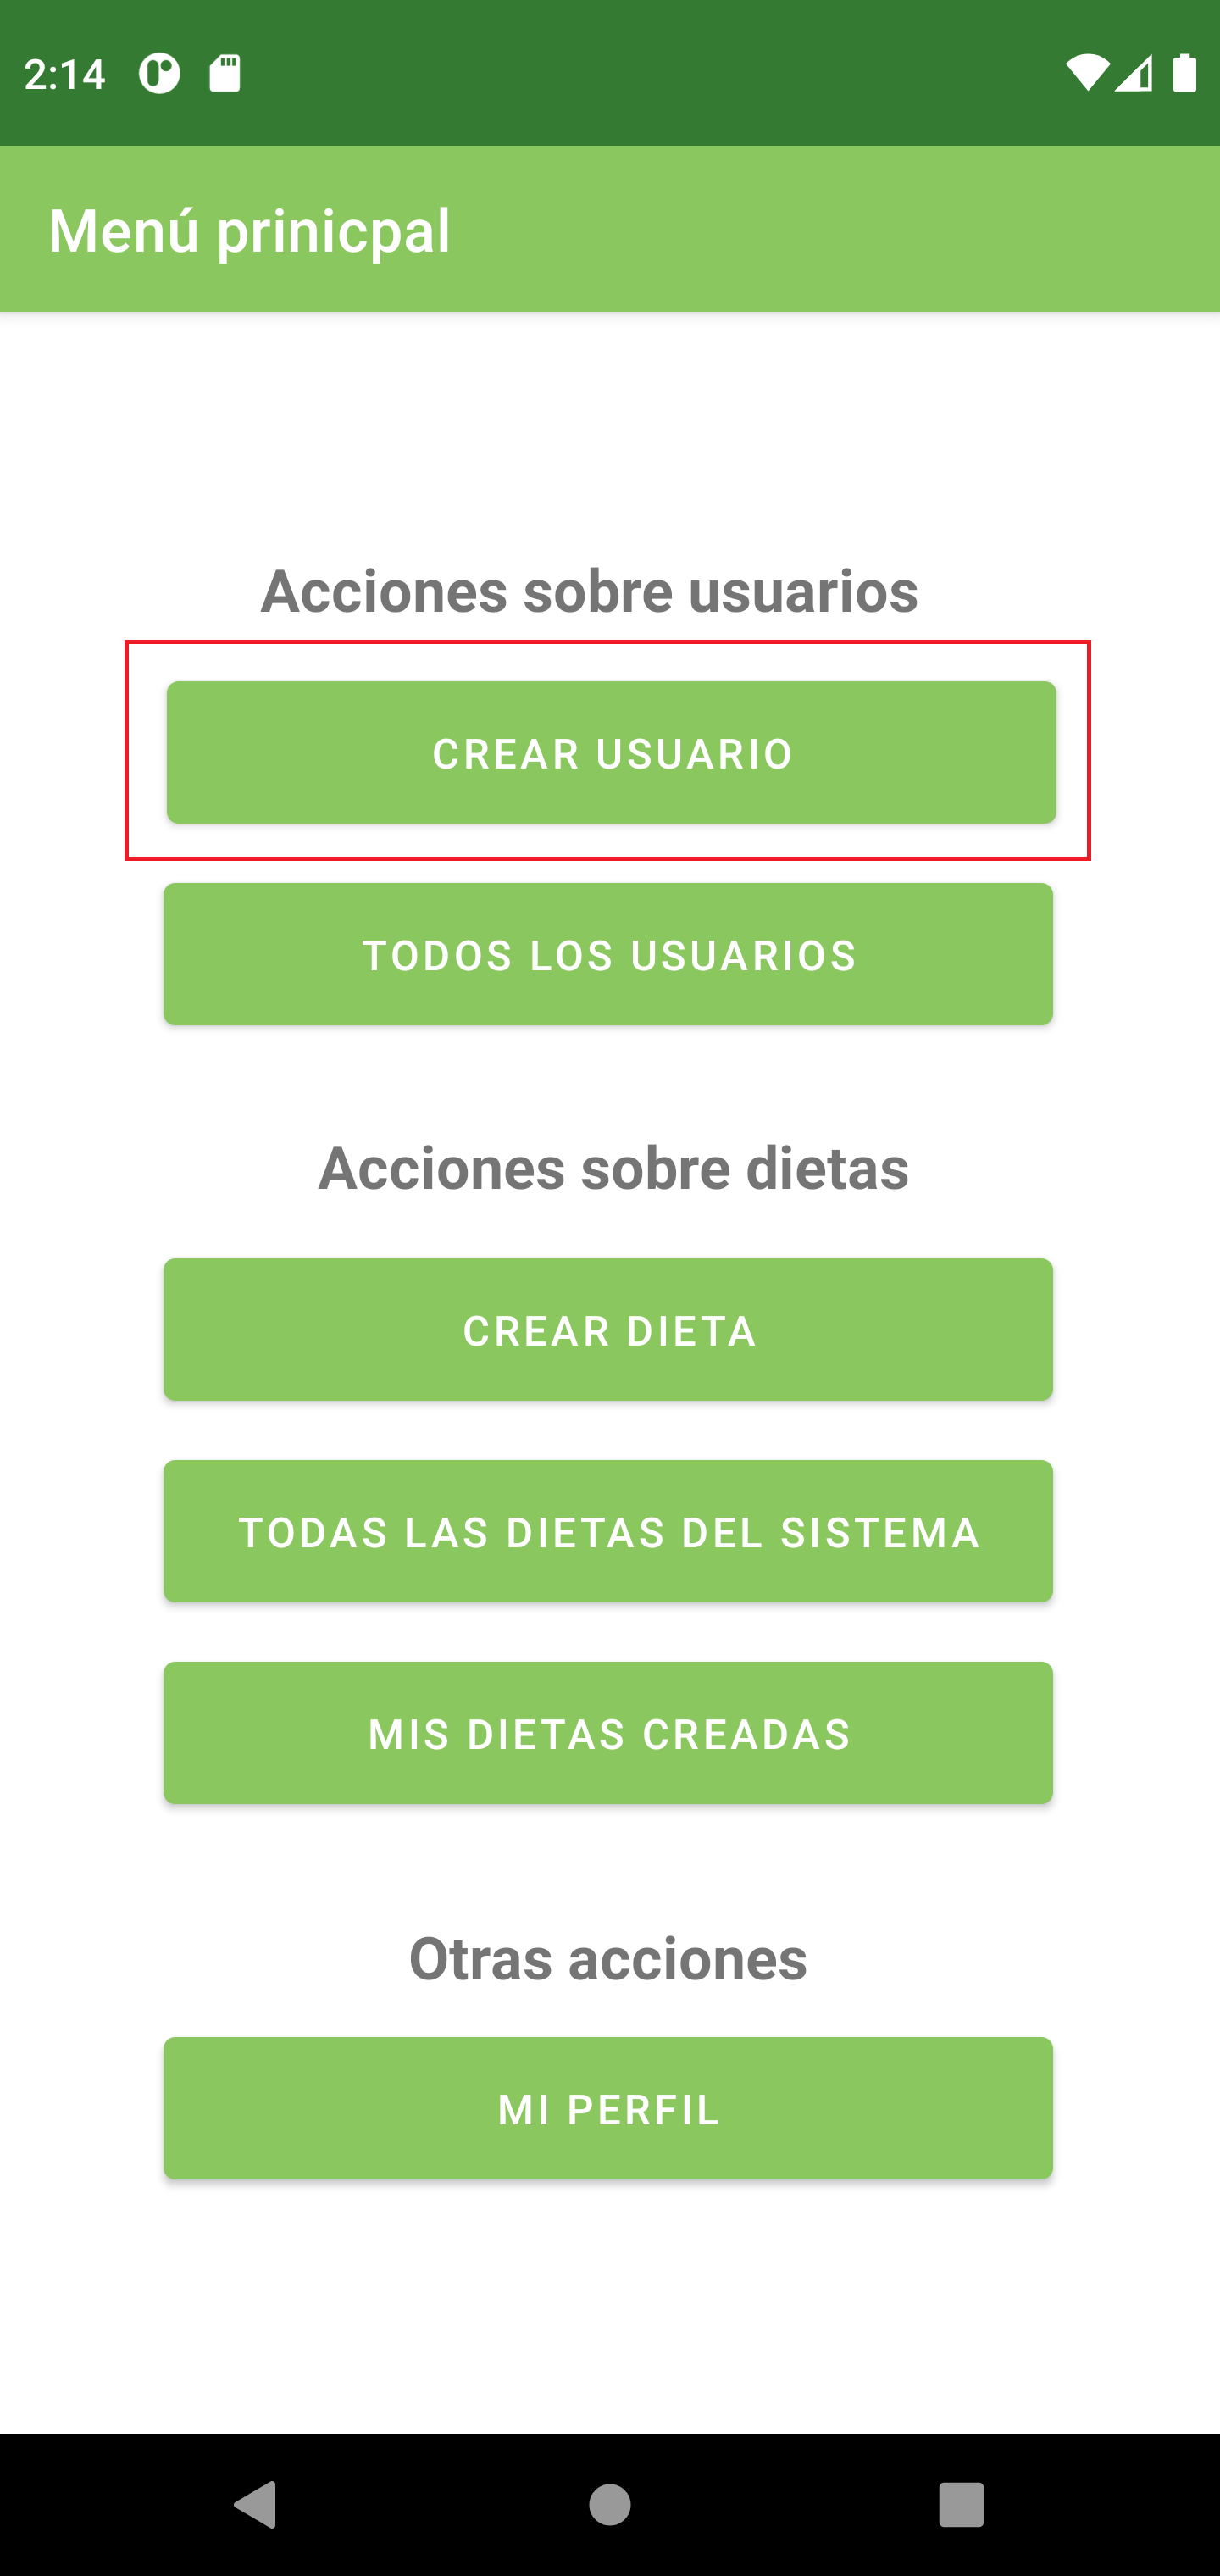
\includegraphics[width=0.4\textwidth]{Images/Annexes/createUsers.png}}
    \subfigure{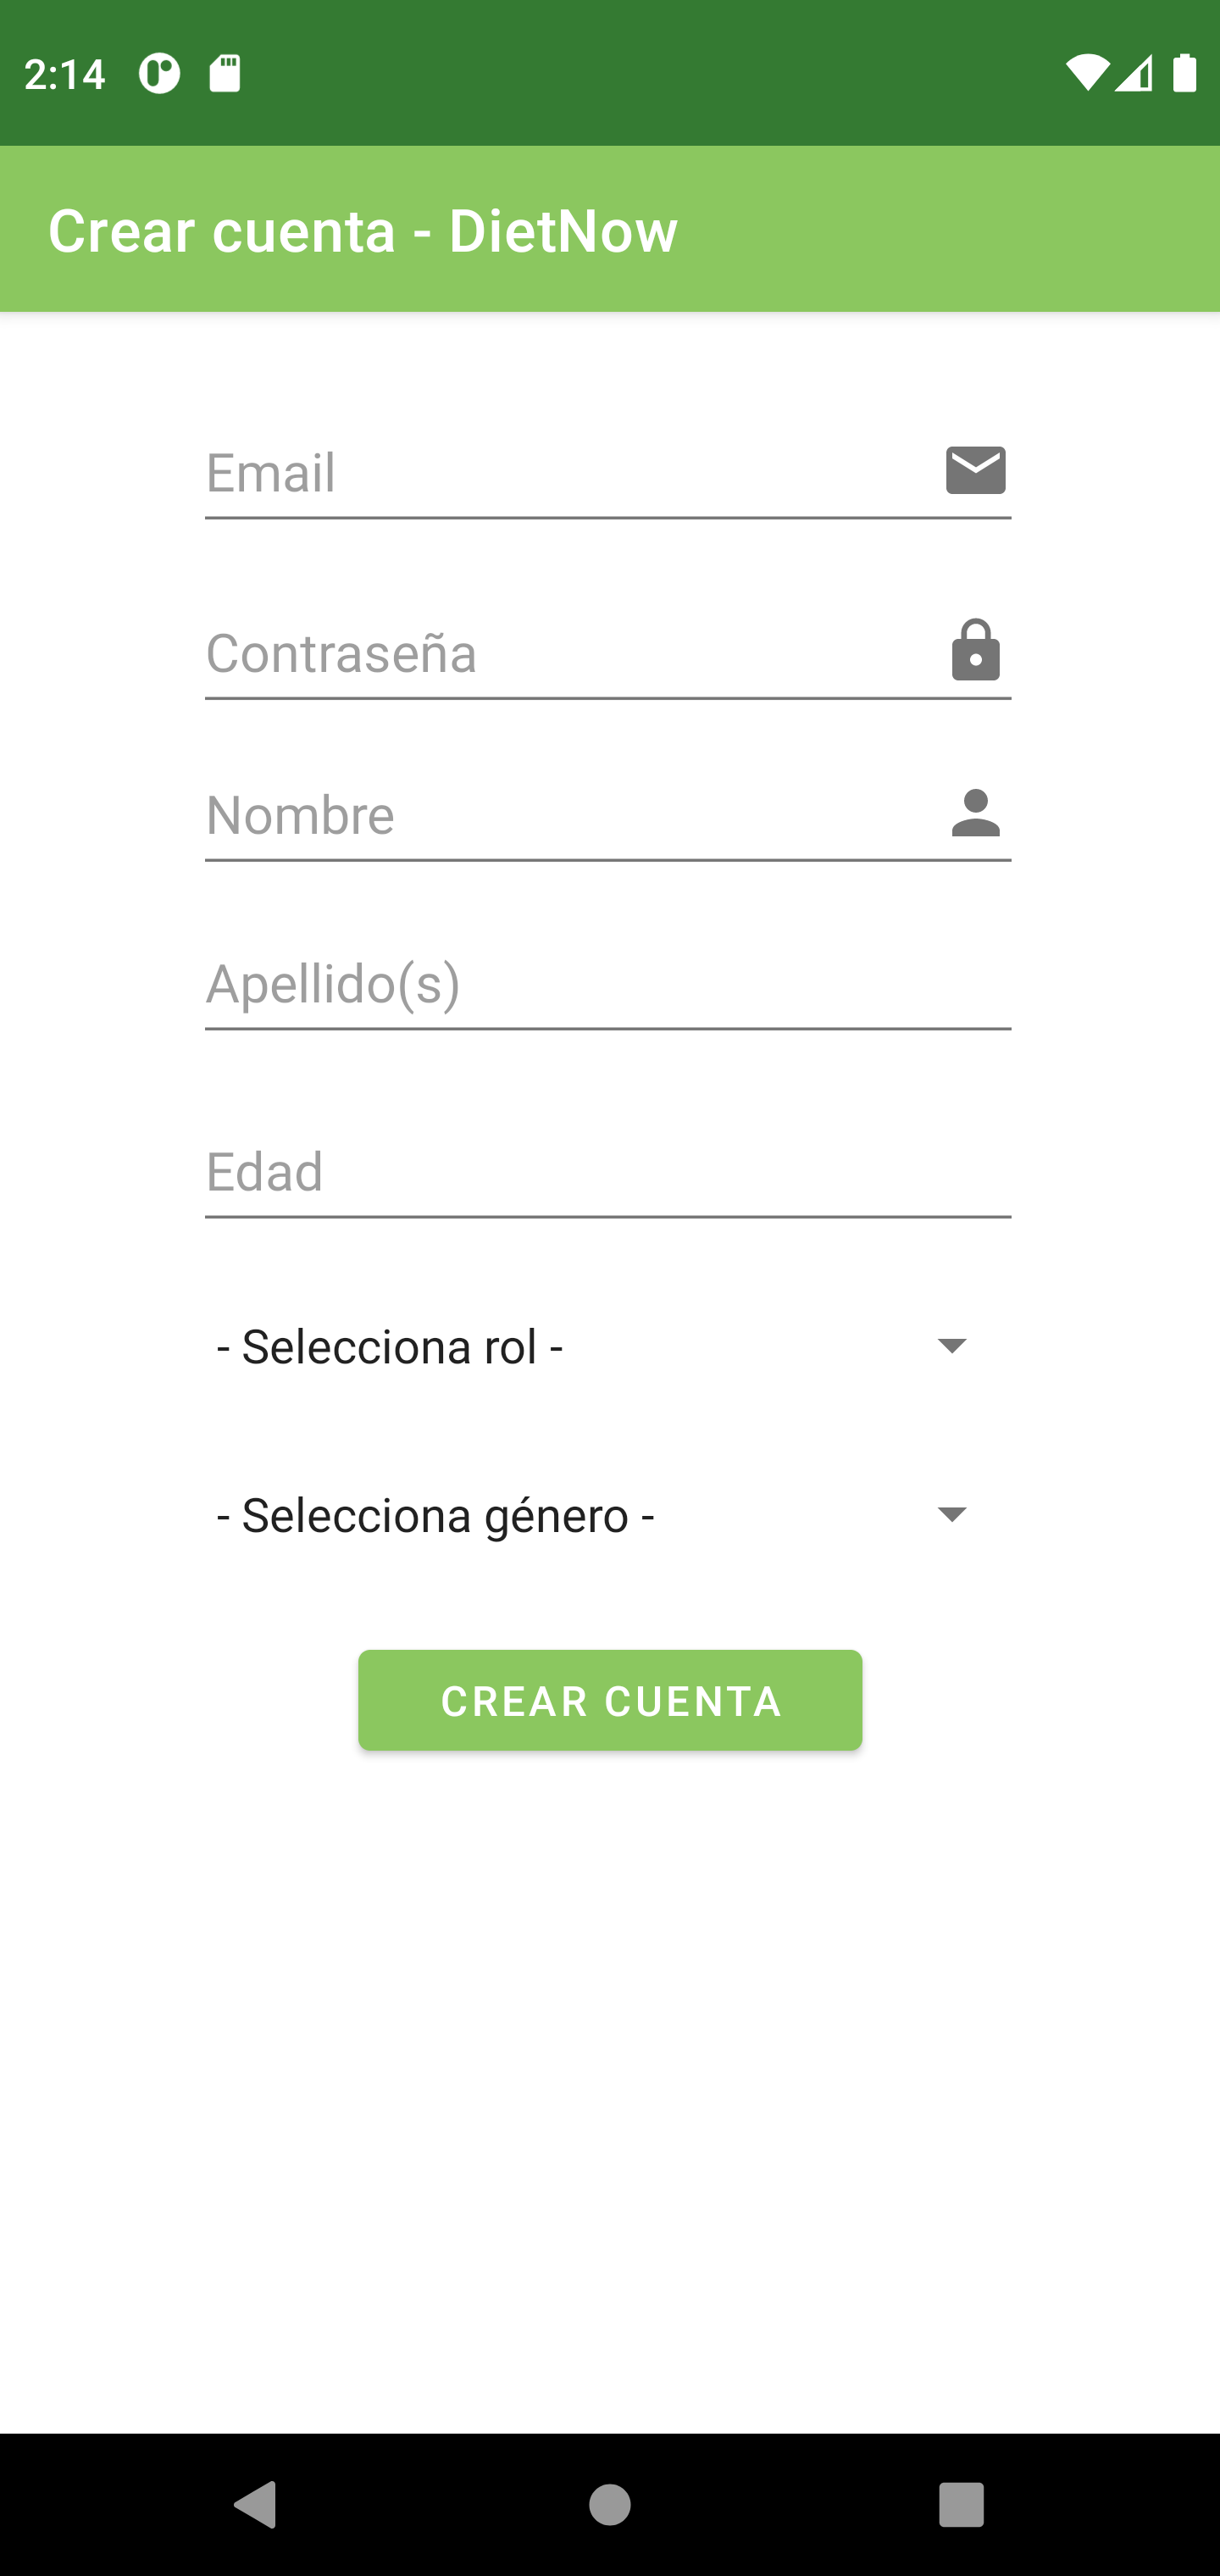
\includegraphics[width=0.4\textwidth]{Images/Annexes/createUsers2.png}}
    \caption{Creación de un usuario en la aplicación}
    \label{fig:crear_usuario_admin}
\end{figure}


\subsection{Todos los usuarios}
Si el administrador selecciona esta opción se abrirá en una nueva ventana un listado con todos los usuarios que están dados de alta en la aplicación, como se muestra en la figura \ref{fig:todos_usuarios}. En esta pantalla se puede filtrar dinámicamente a los usuarios mediante la lupa de la parte superior y se puede editar o eliminar a los diferentes usuarios de la aplicación.

\begin{figure}[H]
    \centering
    \subfigure{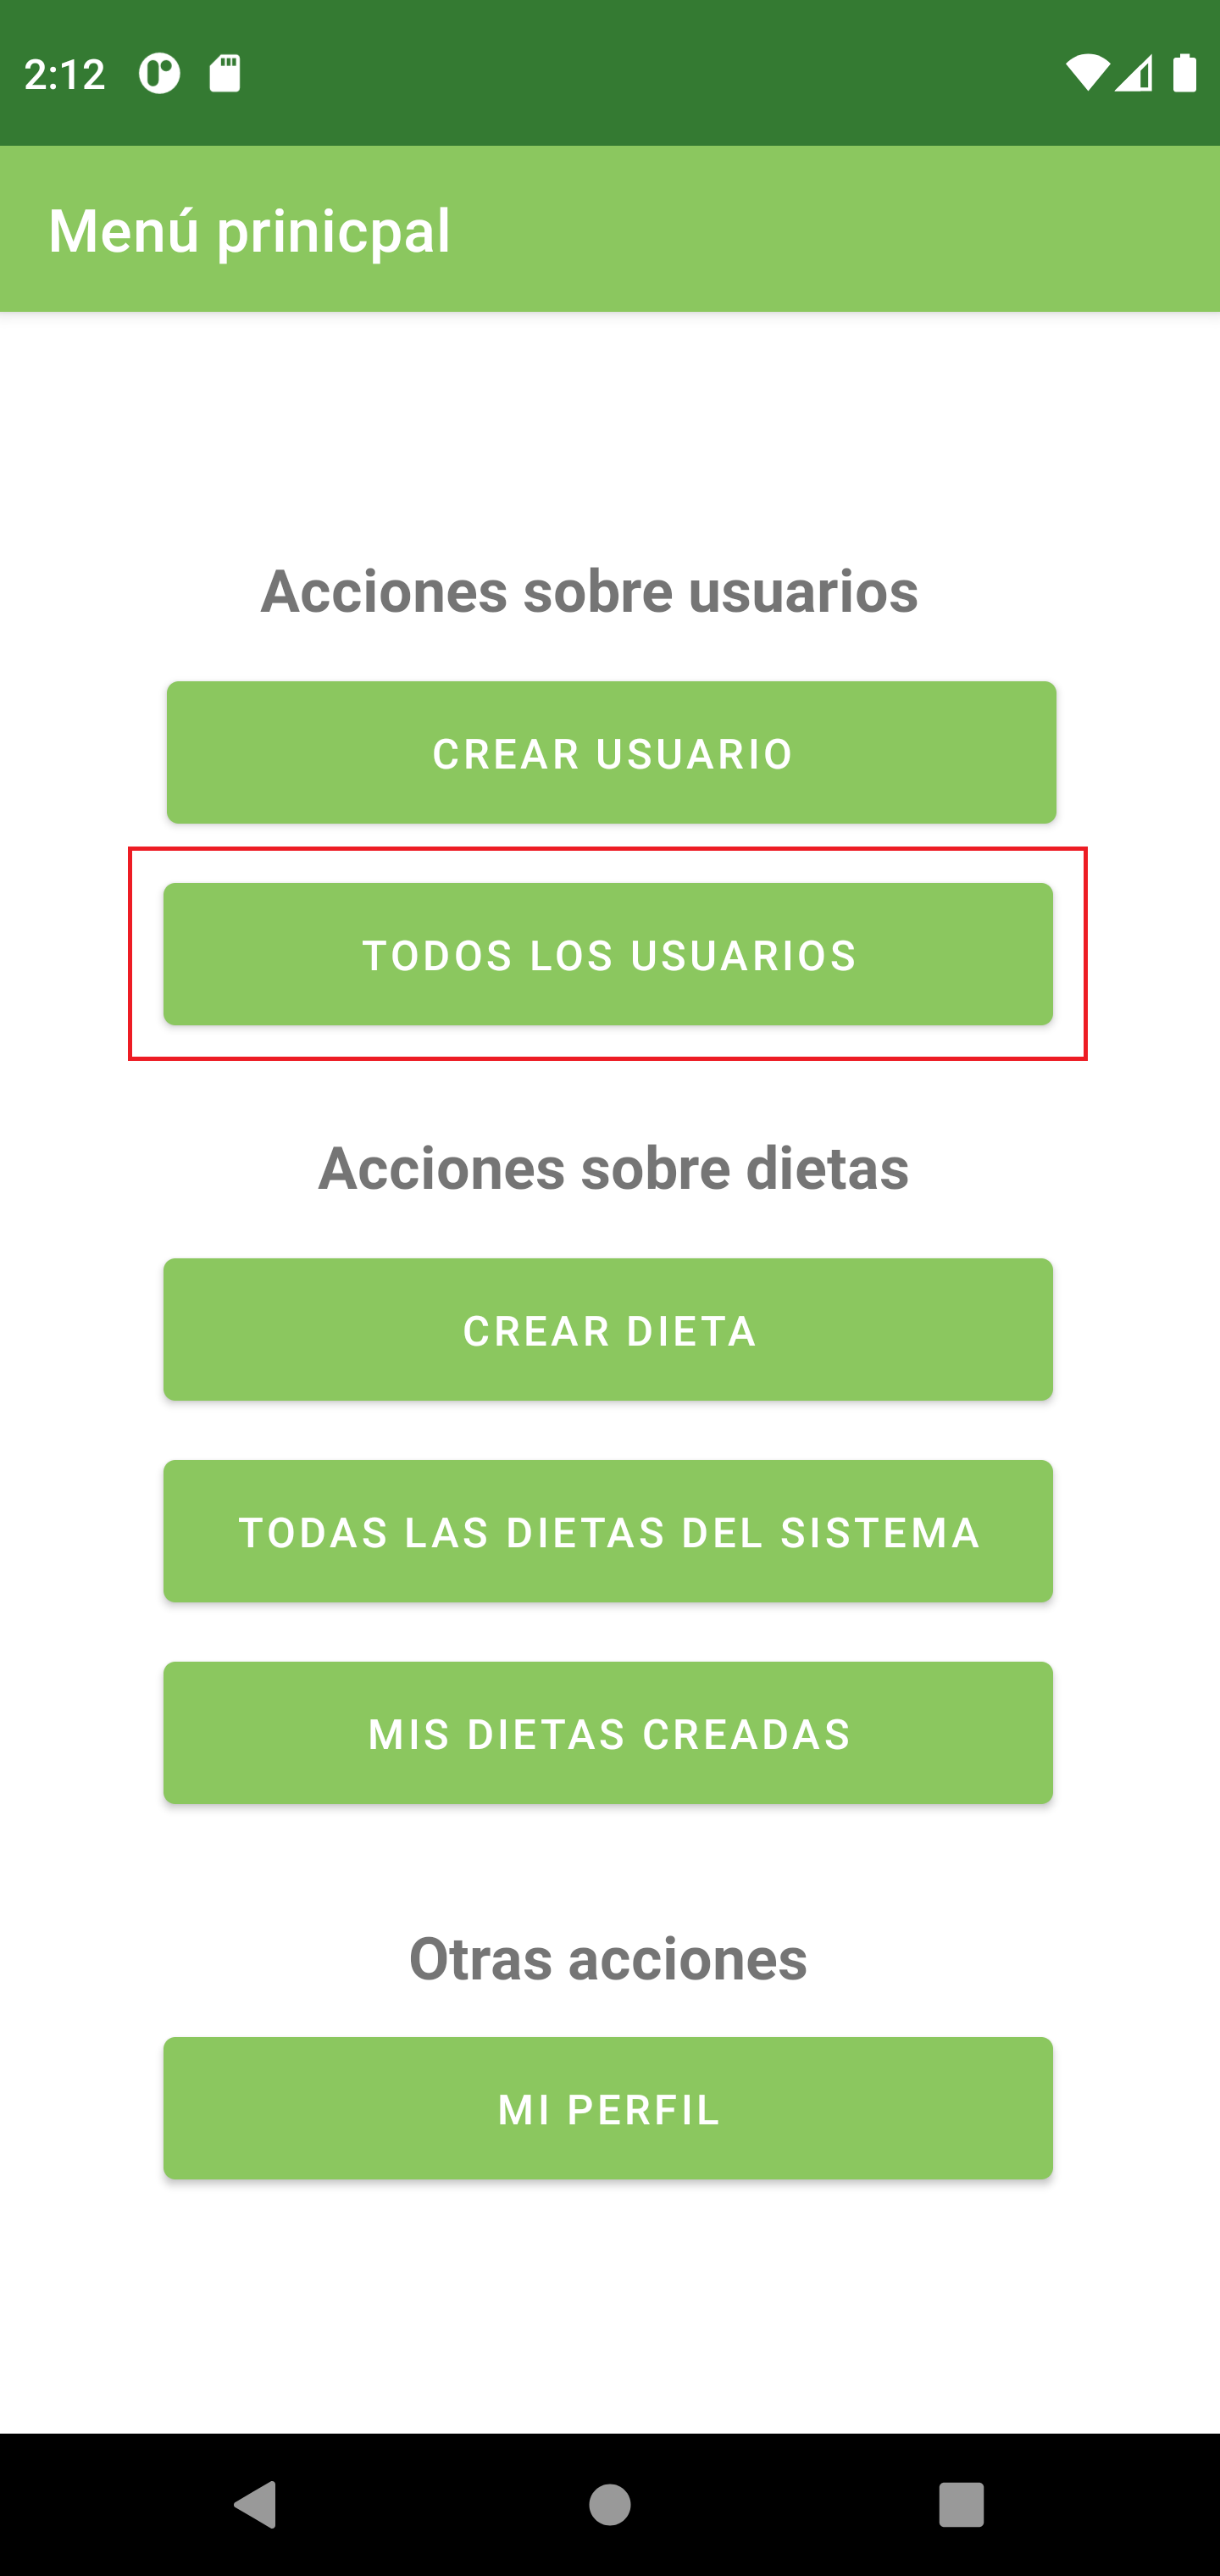
\includegraphics[width=0.4\textwidth]{Images/Annexes/allUsersAdmin.png}}
    \subfigure{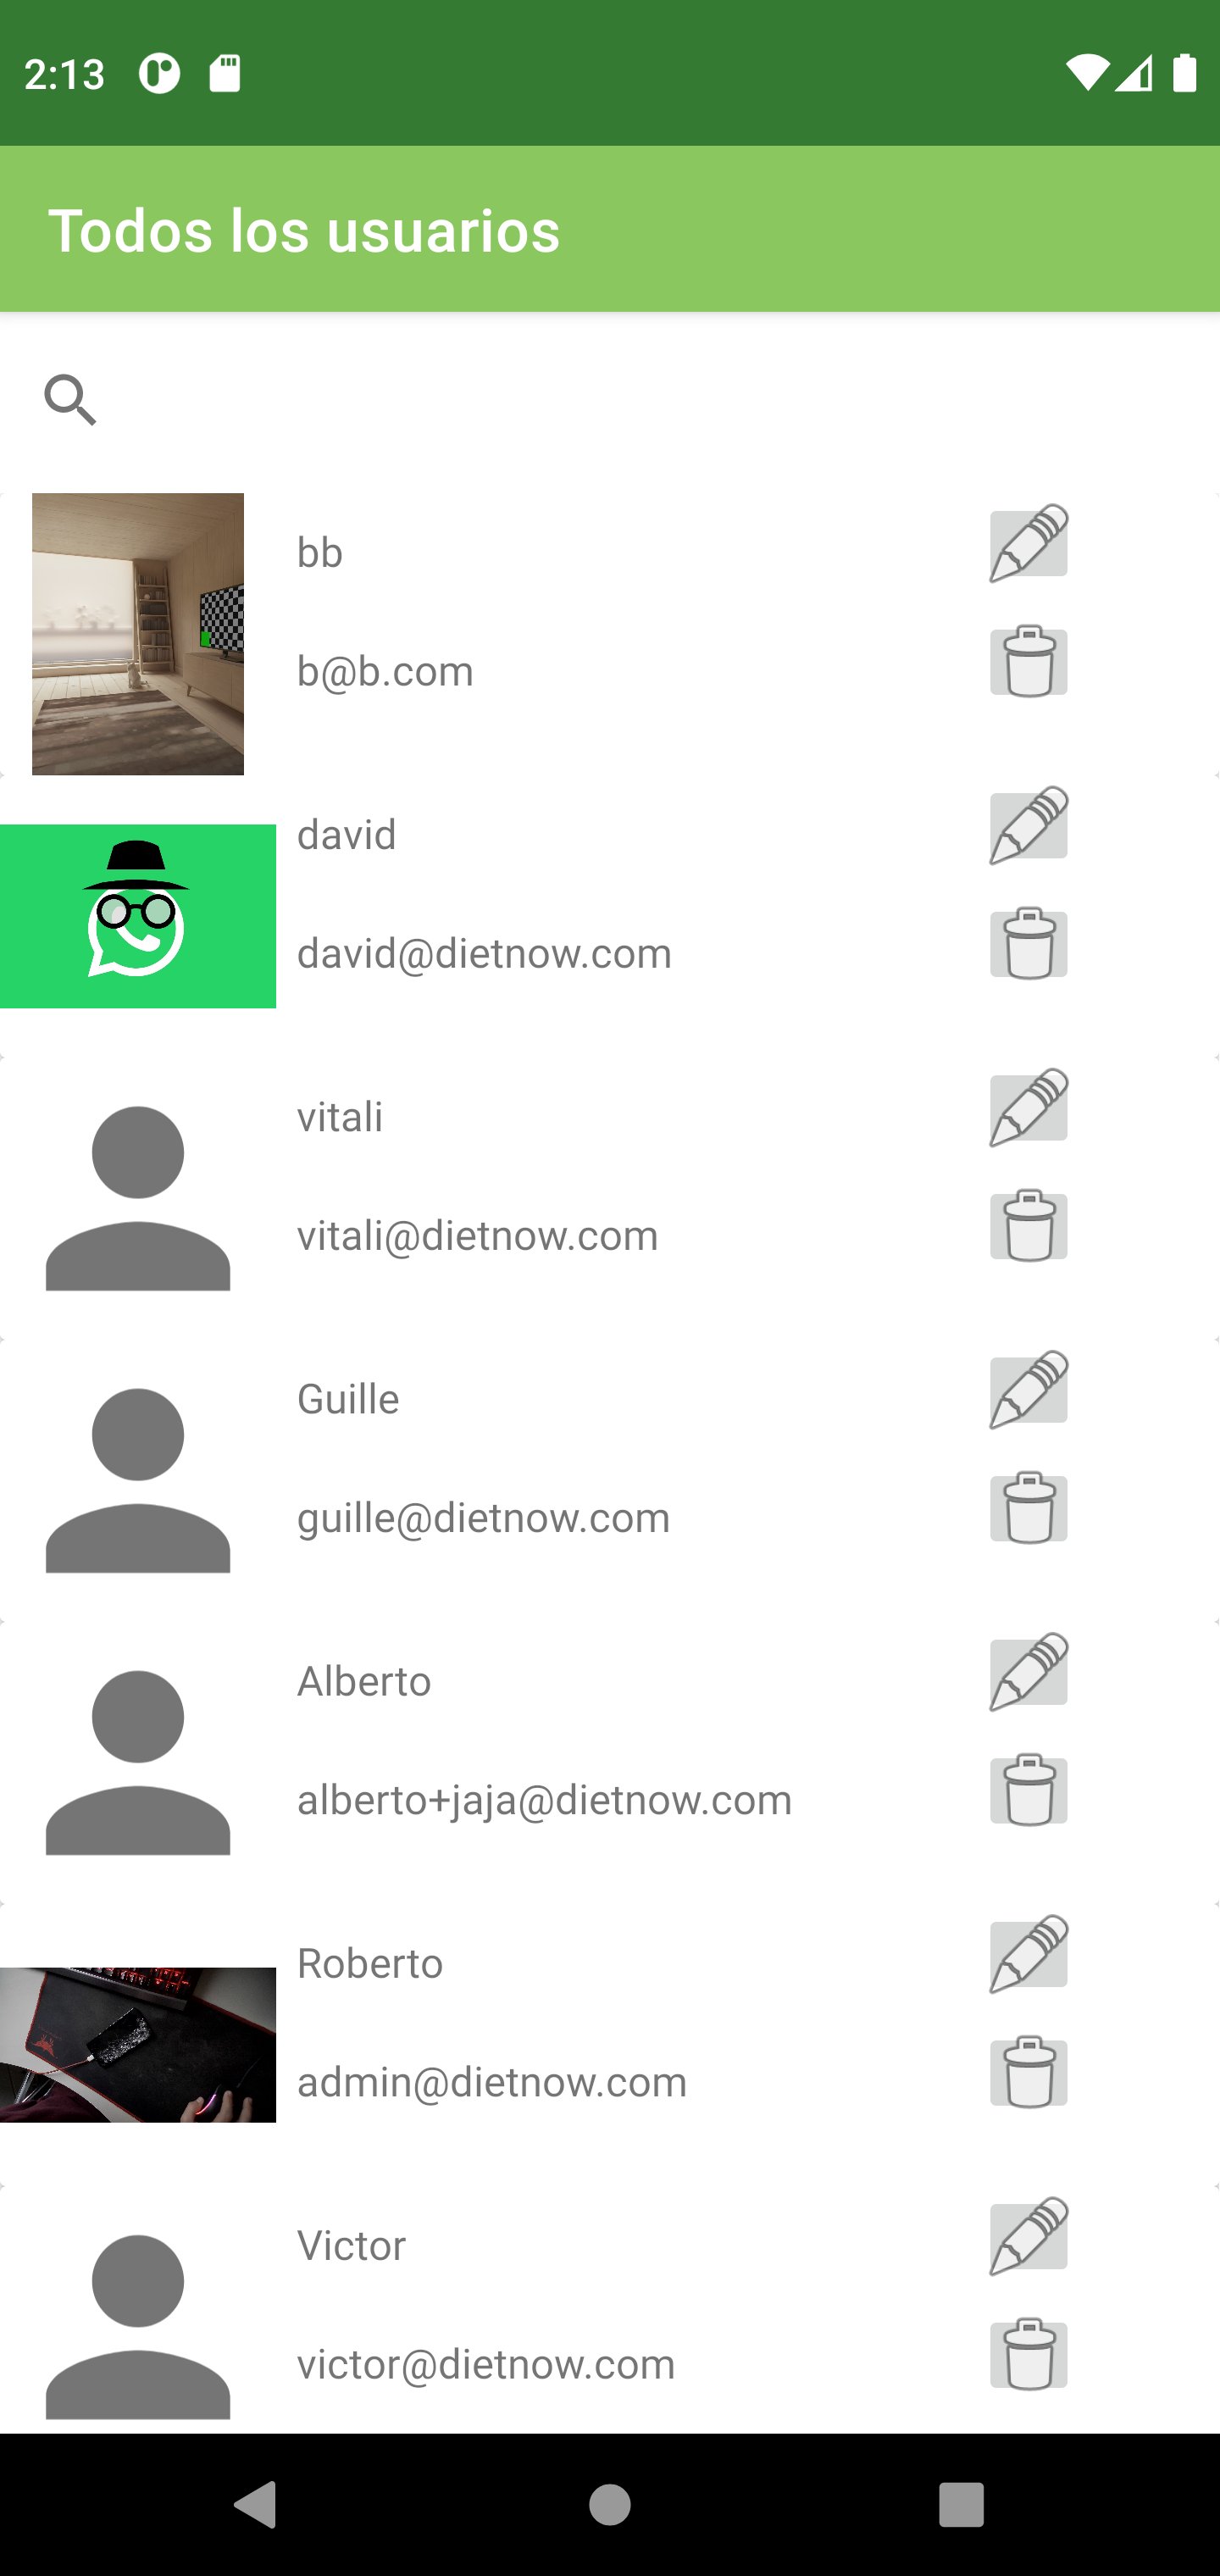
\includegraphics[width=0.4\textwidth]{Images/Annexes/allUsersAdmin2.png}}
    \caption{Vista de todos los usuarios}
    \label{fig:todos_usuarios}
\end{figure}


\subsection{Crear dieta}
Esta opción abre el formulario de creación de dieta, como se muestra en la figura \ref{fig:crear_dieta}, idéntico a cuando en el módulo ``Mis dietas creadas`` un usuario pulsa el botón circular con el símbolo ``$+$``.

\begin{figure}[H]
    \centering
    \subfigure{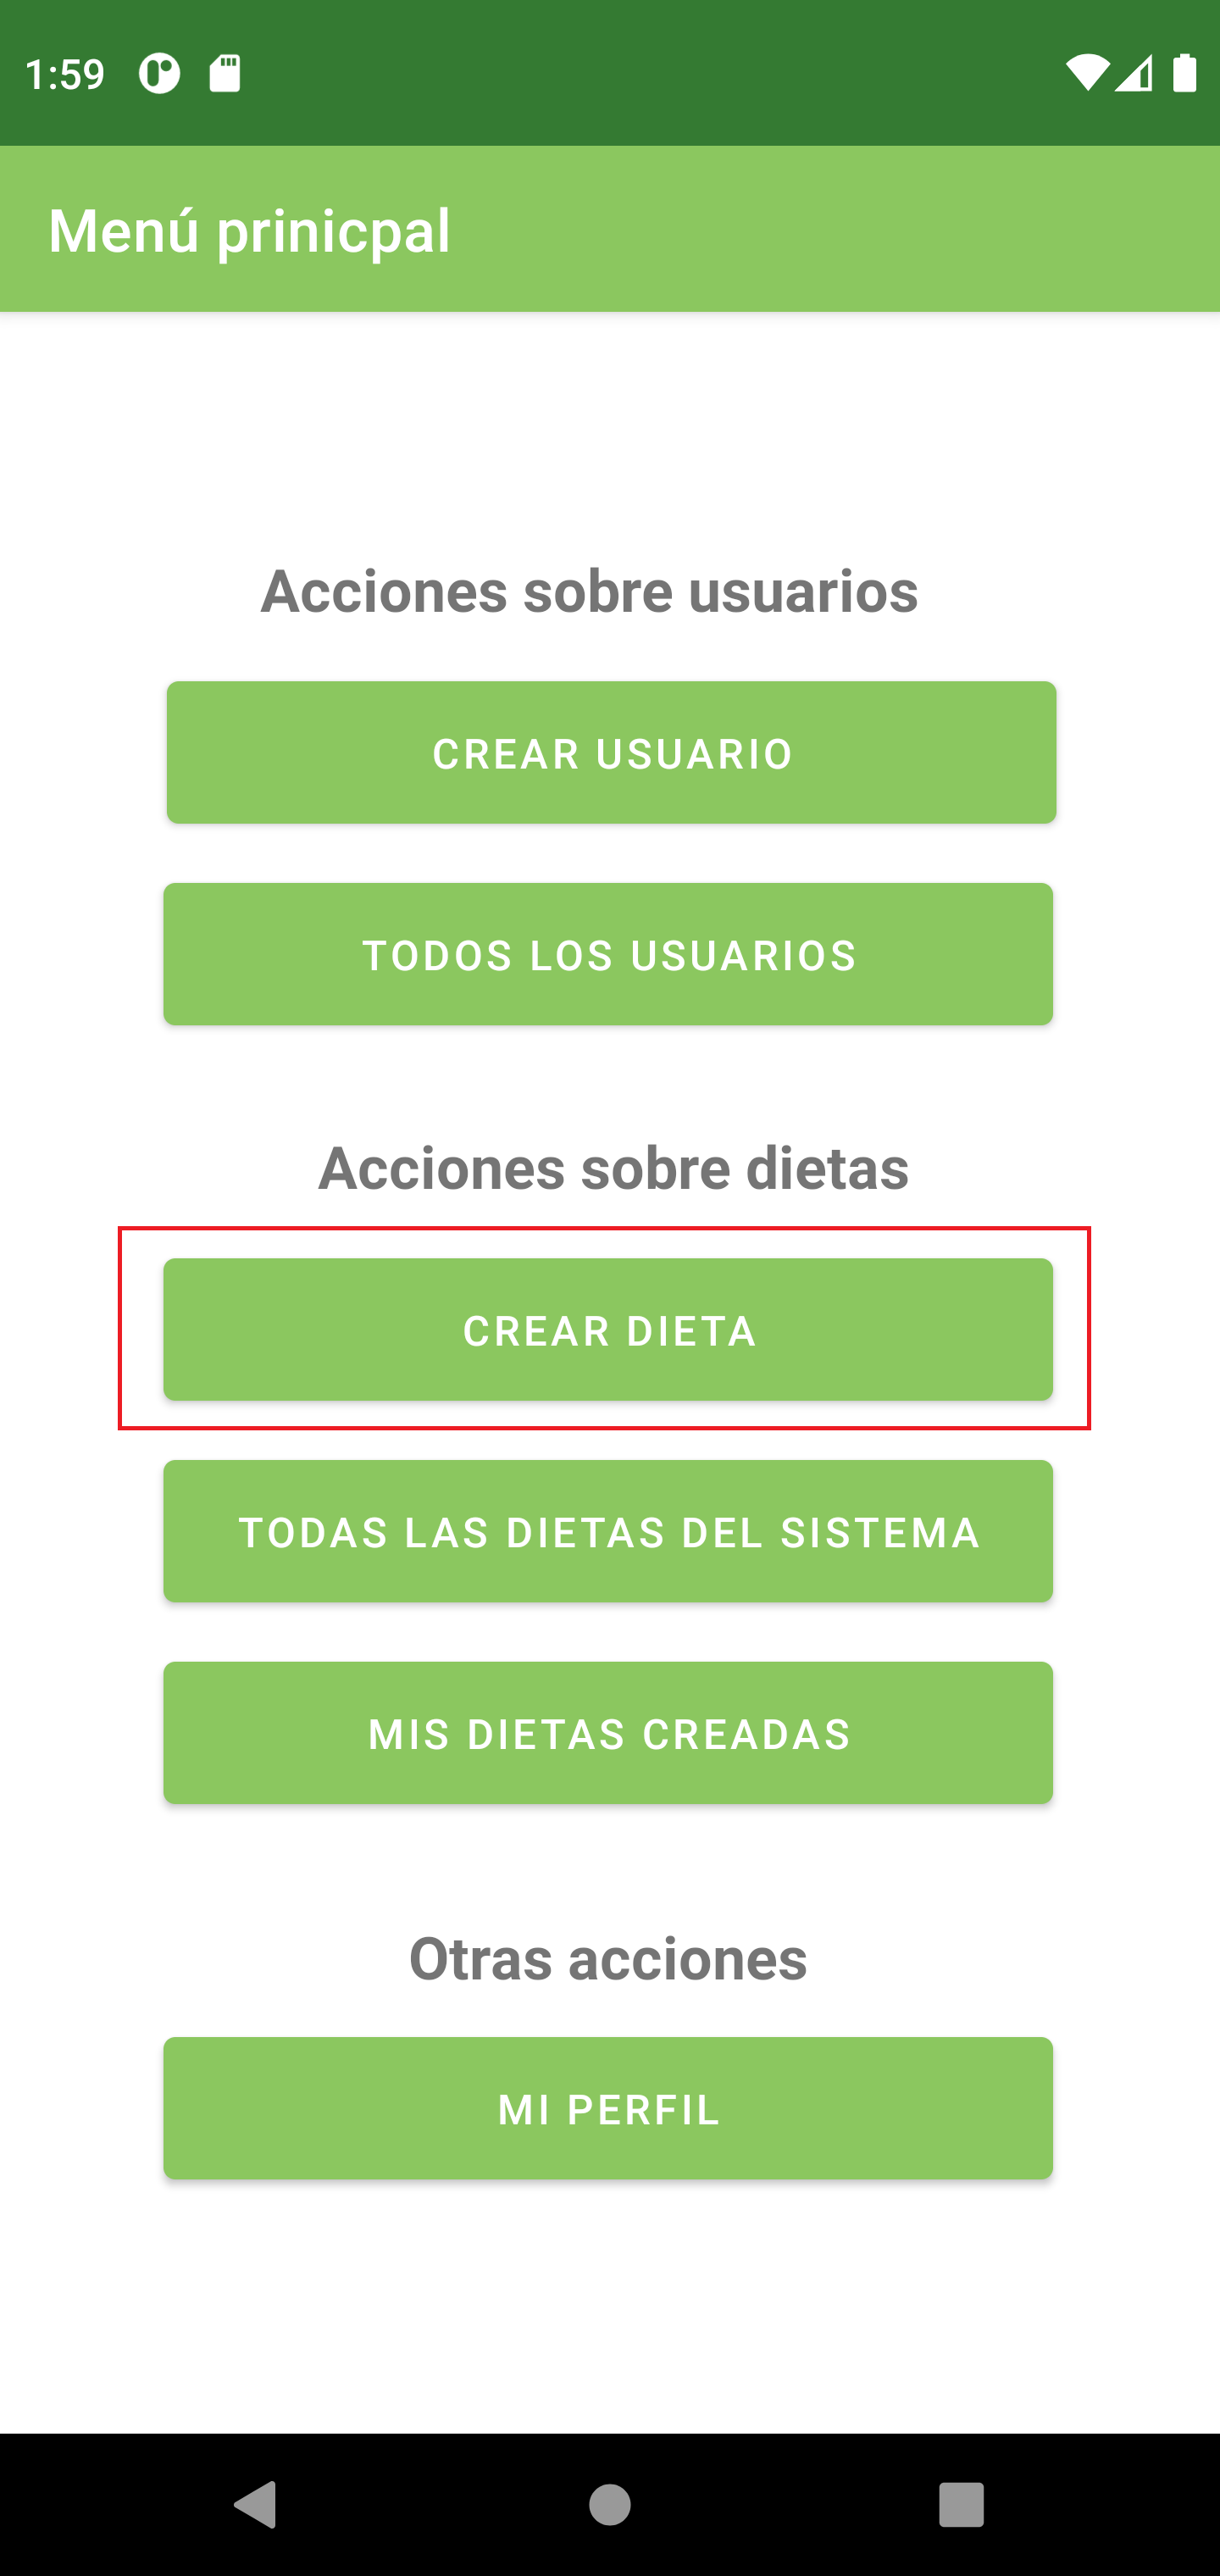
\includegraphics[width=0.4\textwidth]{Images/Annexes/adminCreateDiet.png}}
    \subfigure{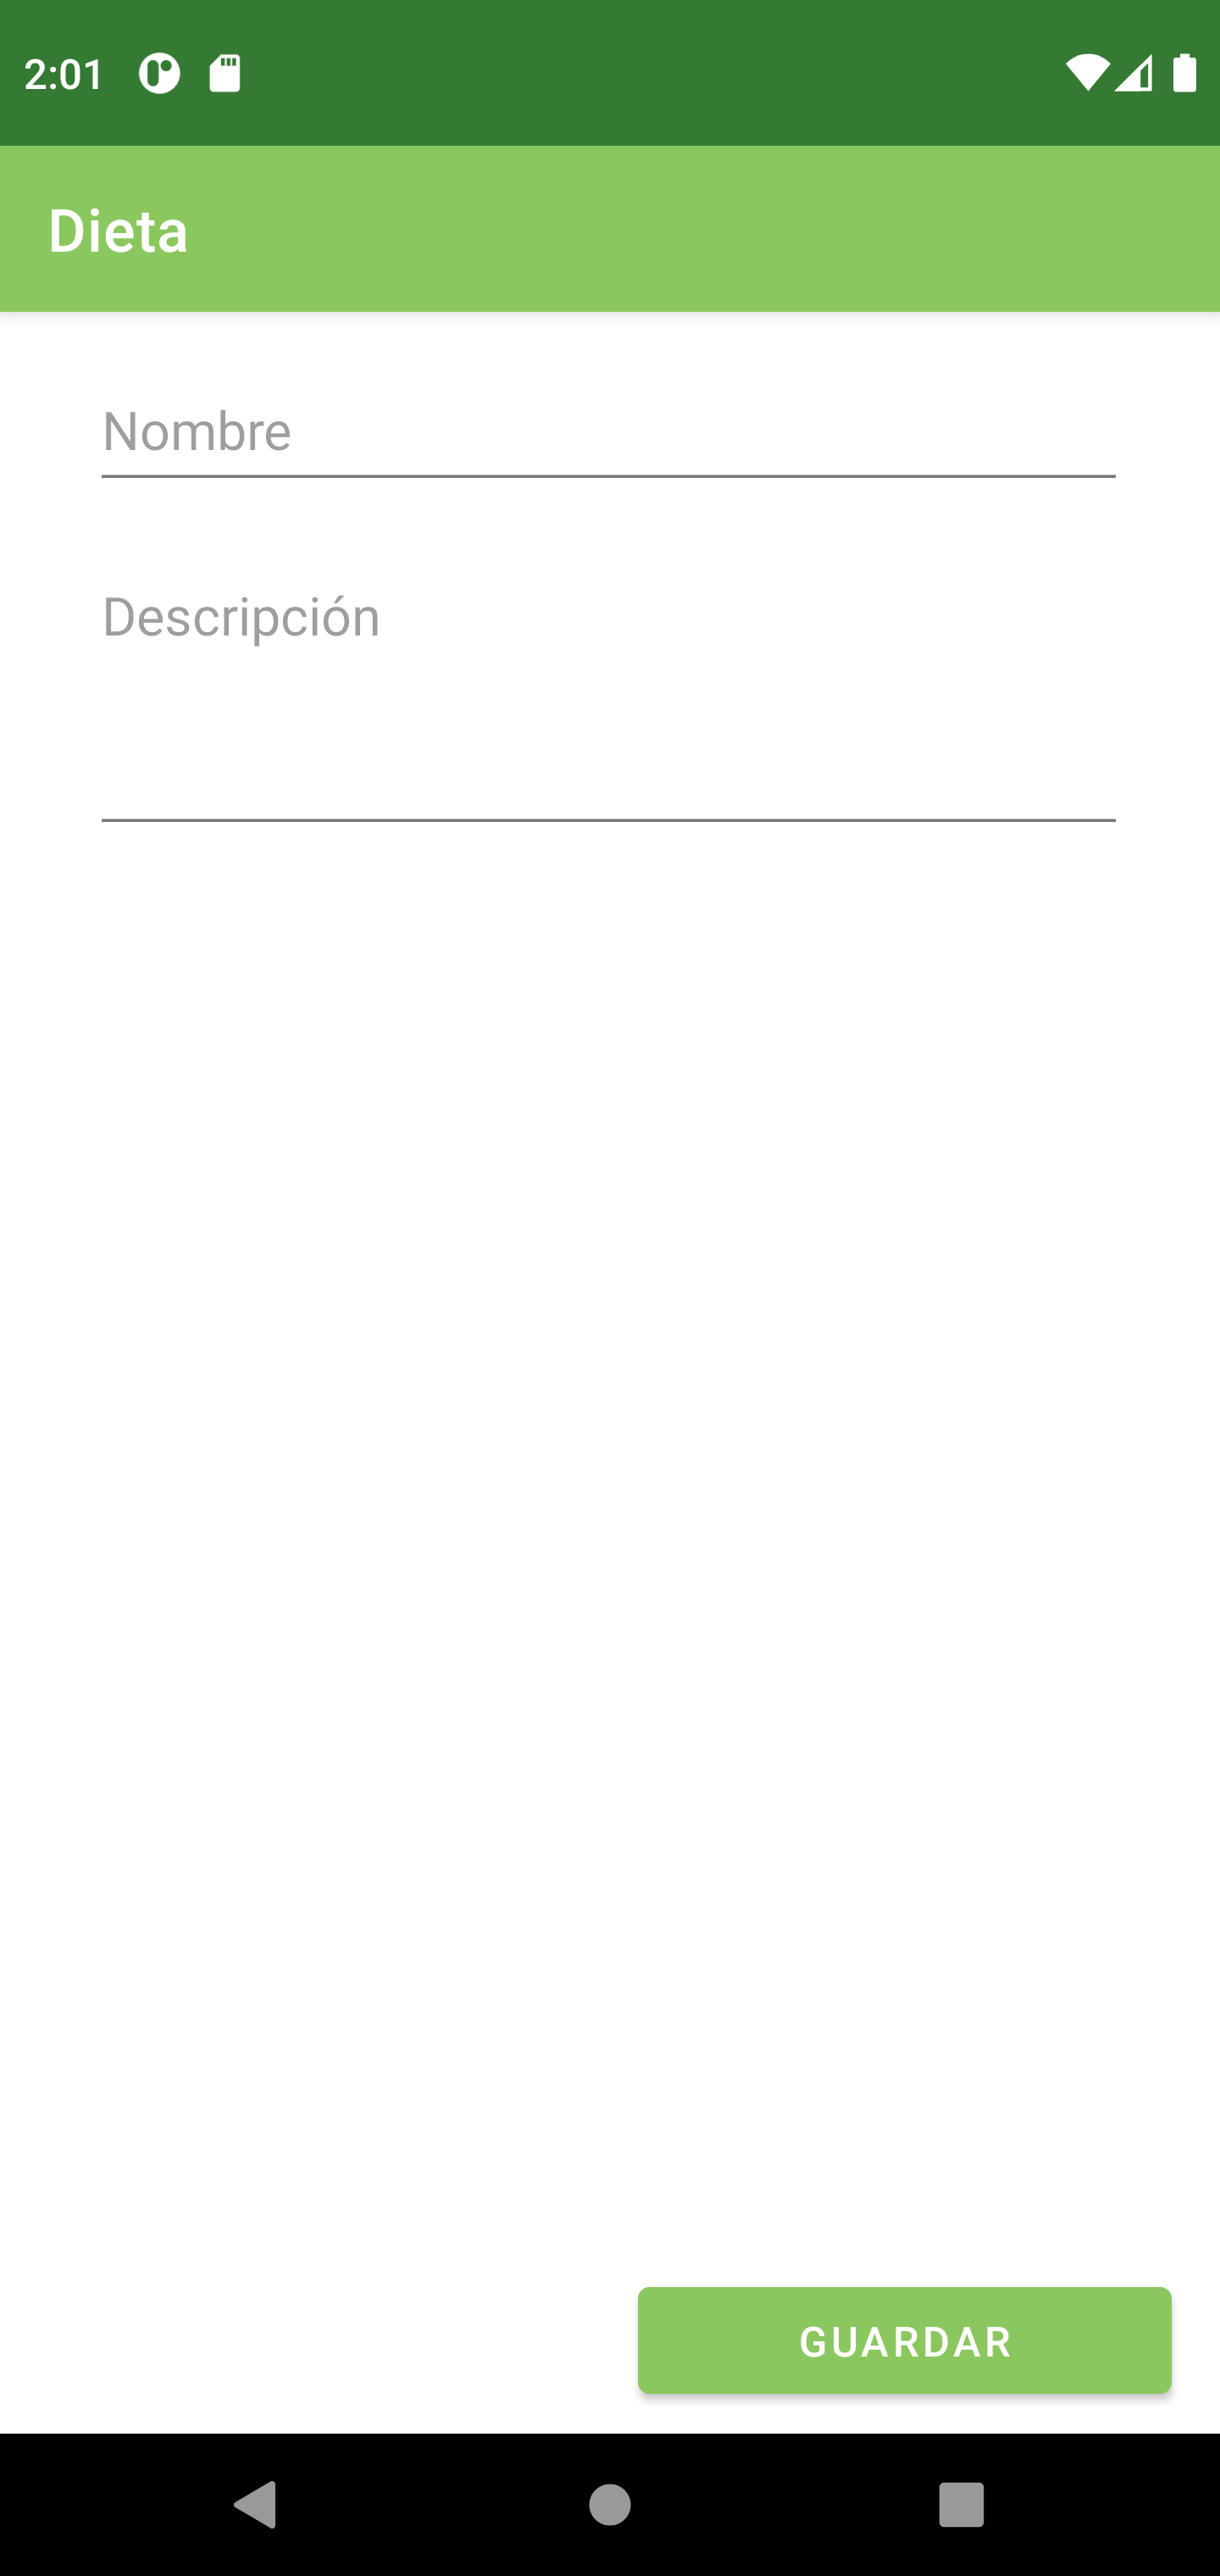
\includegraphics[width=0.4\textwidth]{Images/Annexes/adminCreateDiet2.png}}
    \caption{Crear una dieta}
    \label{fig:crear_dieta}
\end{figure}


\subsection{Todas las dietas del sistema}
Mediante esta opción el administrador puede ver todas las dietas de la aplicación \ref{fig:todas_dietas}, tanto las publicadas como las privadas, al seleccionar la opción se le mostrará un listado con todas las dietas, el número de me gustas y vistos de cada dieta y su estado, es decir si esta publicada o no, también dispondrá de un filtro dinámico en la parte superior de la vista para filtrar las dietas.

El administrador podrá acceder al detalle de cada dieta pulsando ``Ver detalle`` y podrá modificar y/o eliminar la dieta así como cambiar su estado de publicación.

\begin{figure}[H]
    \centering
    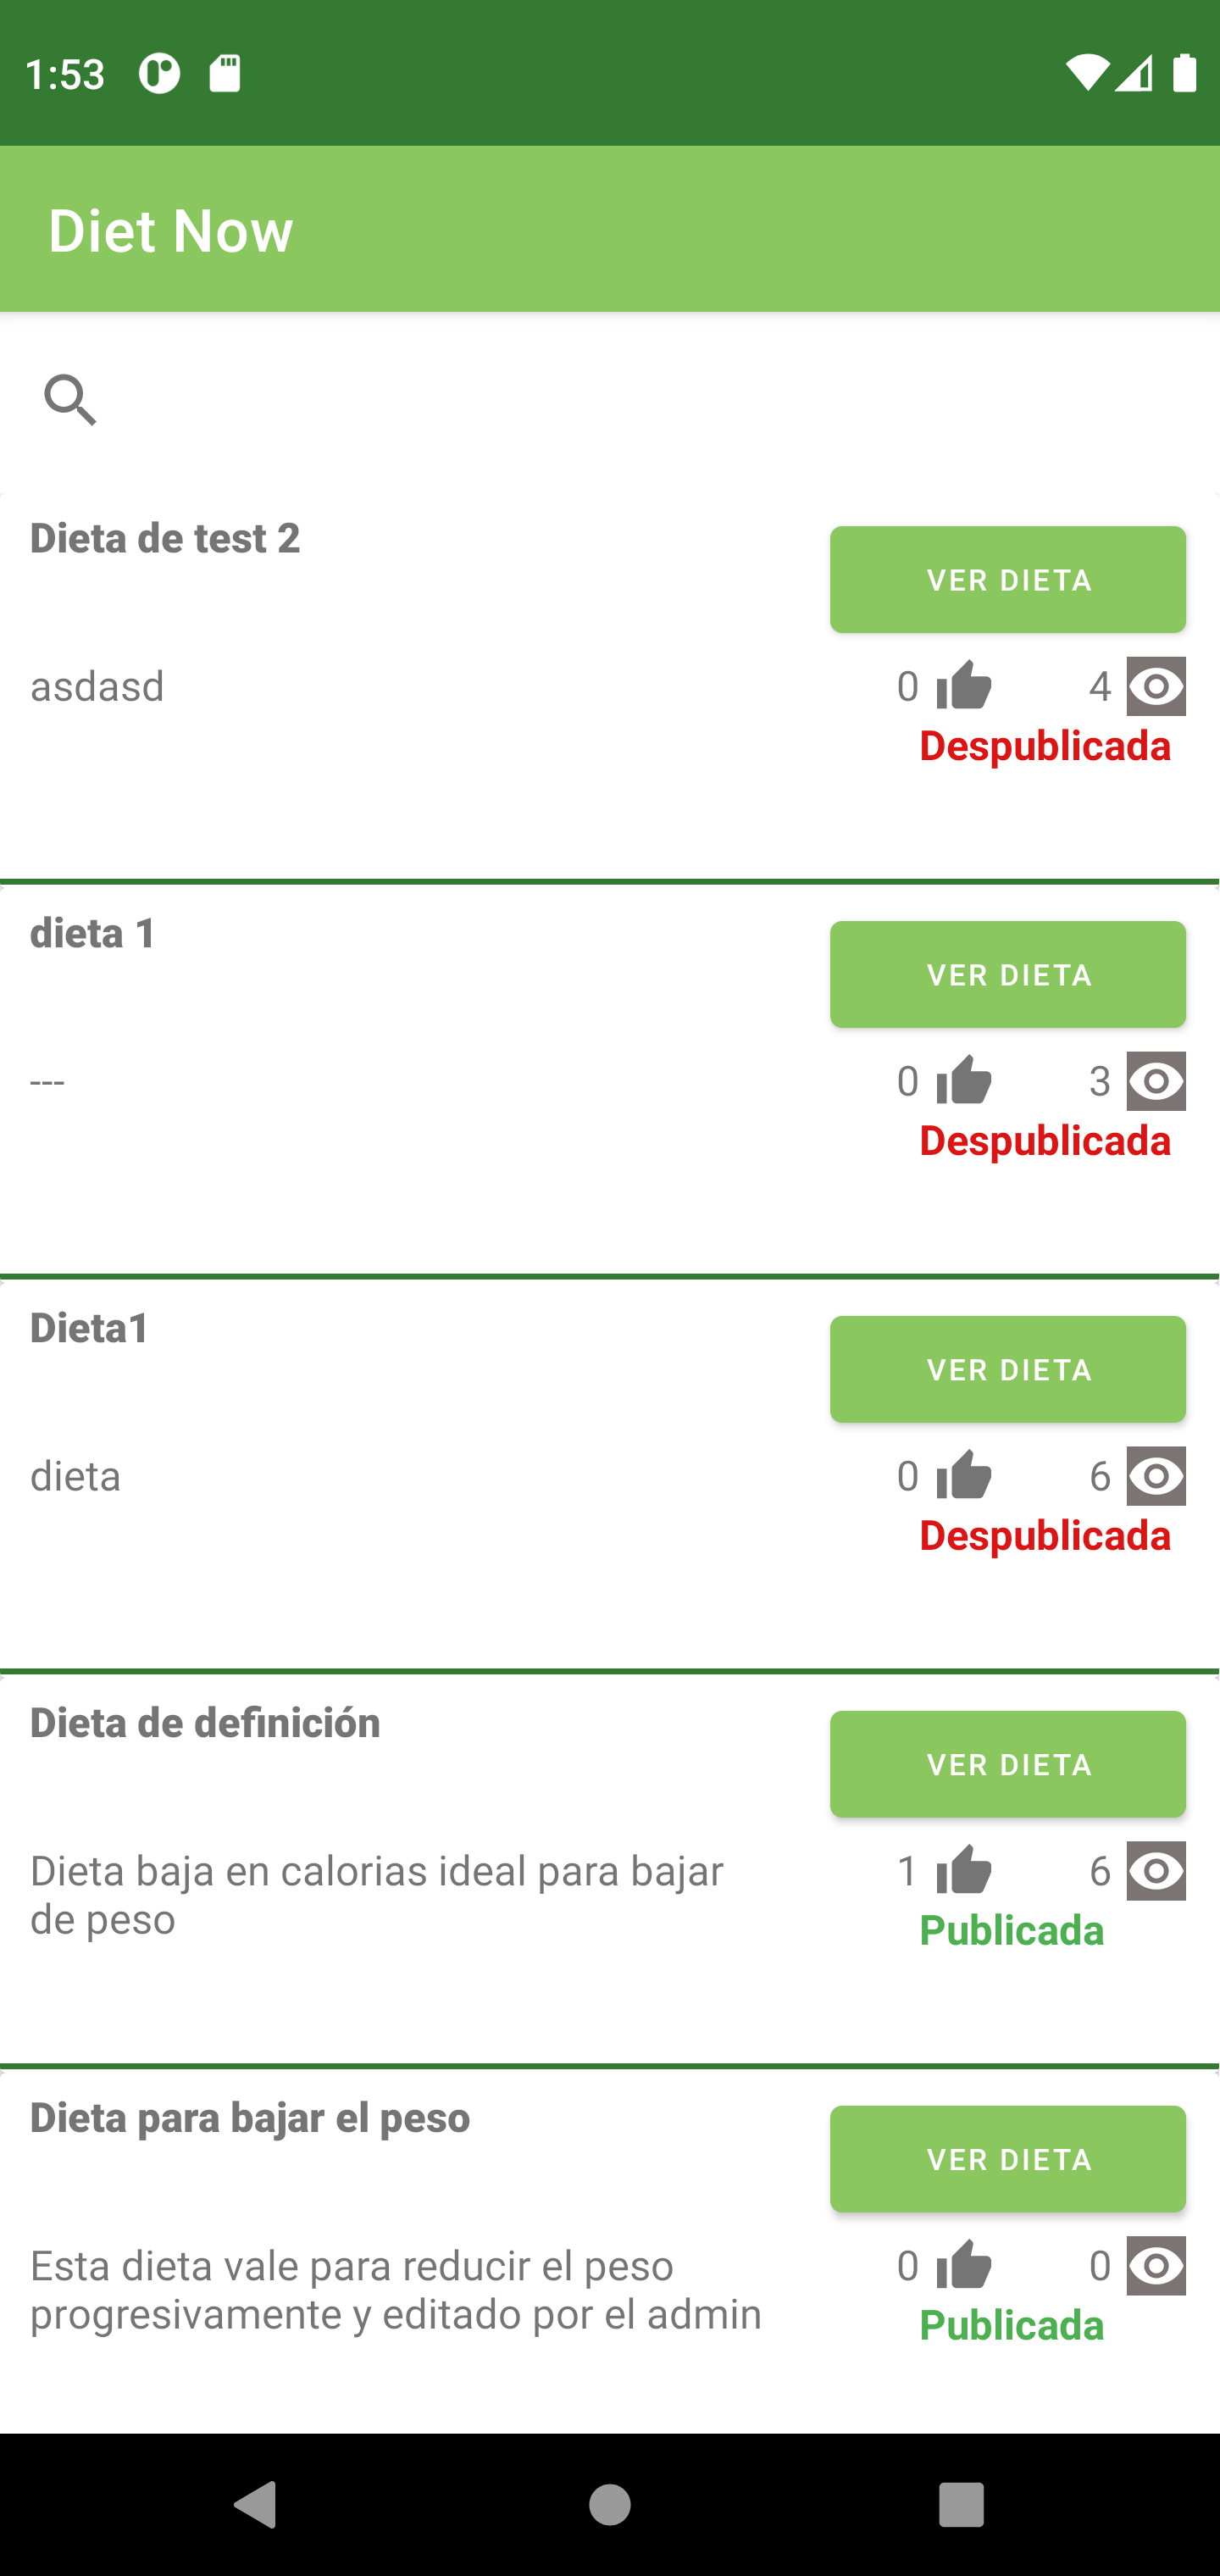
\includegraphics[width=0.4\textwidth]{Images/Annexes/allSysDiets.png}
    \caption{Vista de todas las dietas del sistema}
    \label{fig:todas_dietas}
\end{figure}


\subsection{Mis dietas creadas}
El administrador puede desarrollar está acción de la misma manera que lo haría un deportista, como se aprecia en el apartado \ref{user_my_created_diets}.

\subsection{Ver perfil}
Con esta opción, un administrador accede a su perfil donde se mostrará su información personal y la información del sistema, en esta vista podrá cambiar su imagen de perfil, editar su perfil, cerrar sesión y eliminar cuenta.\ref{fig:admin_profile}

\begin{figure}[H]
    \centering
    \subfigure{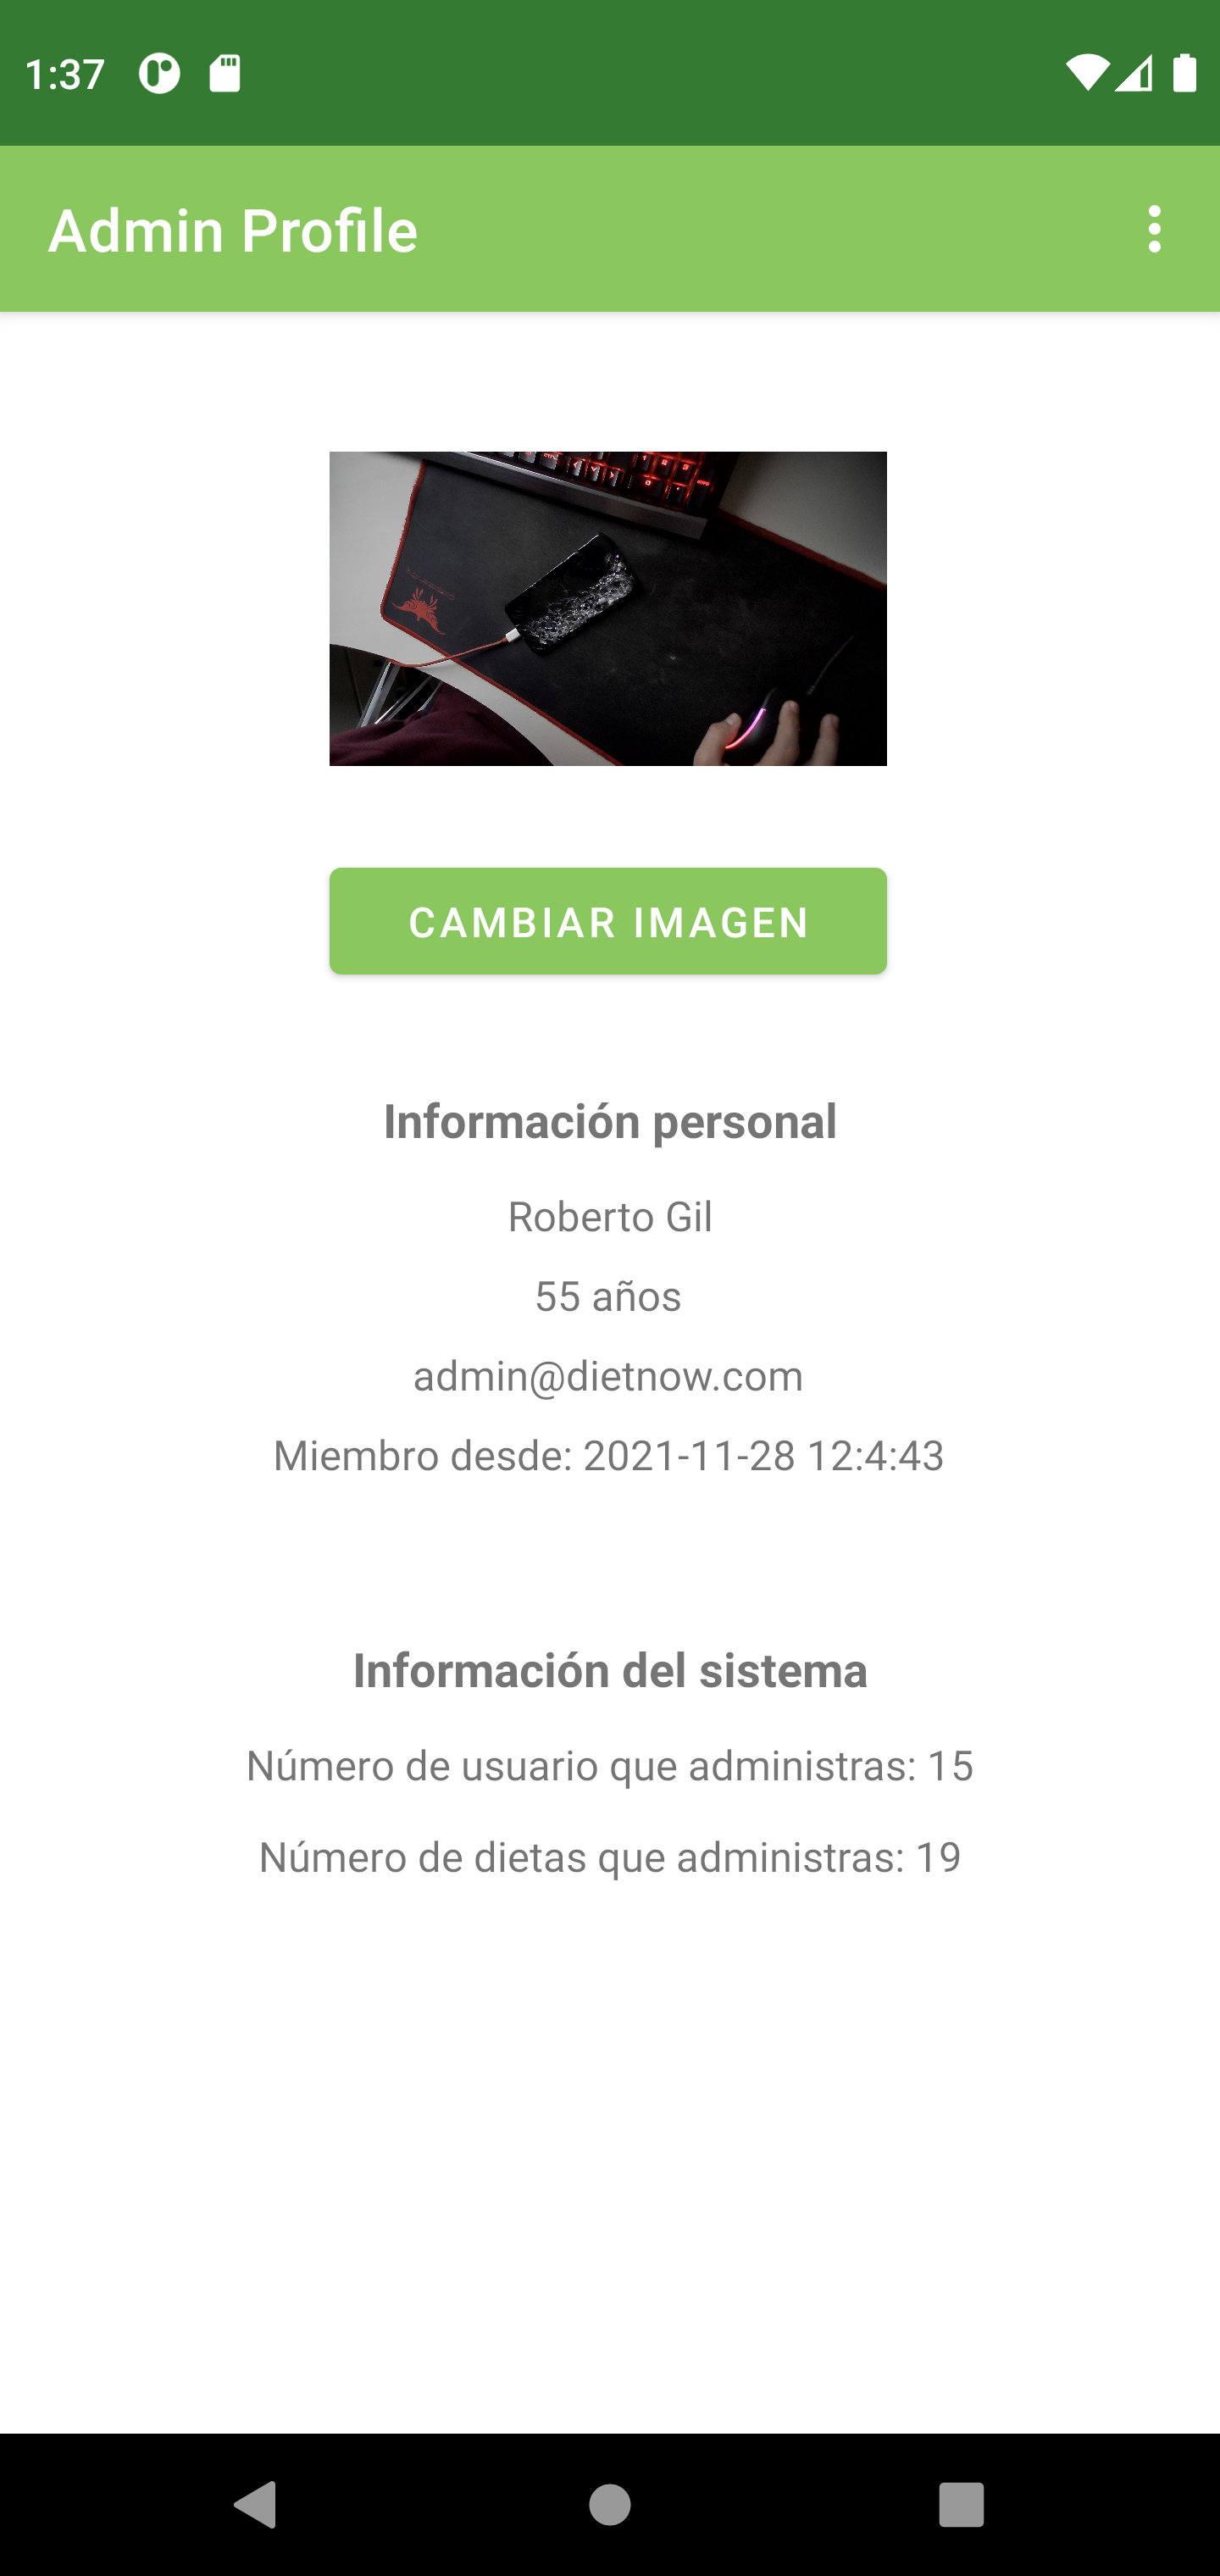
\includegraphics[width=0.4\textwidth]{Images/Annexes/adminProfile.png}}
    \subfigure{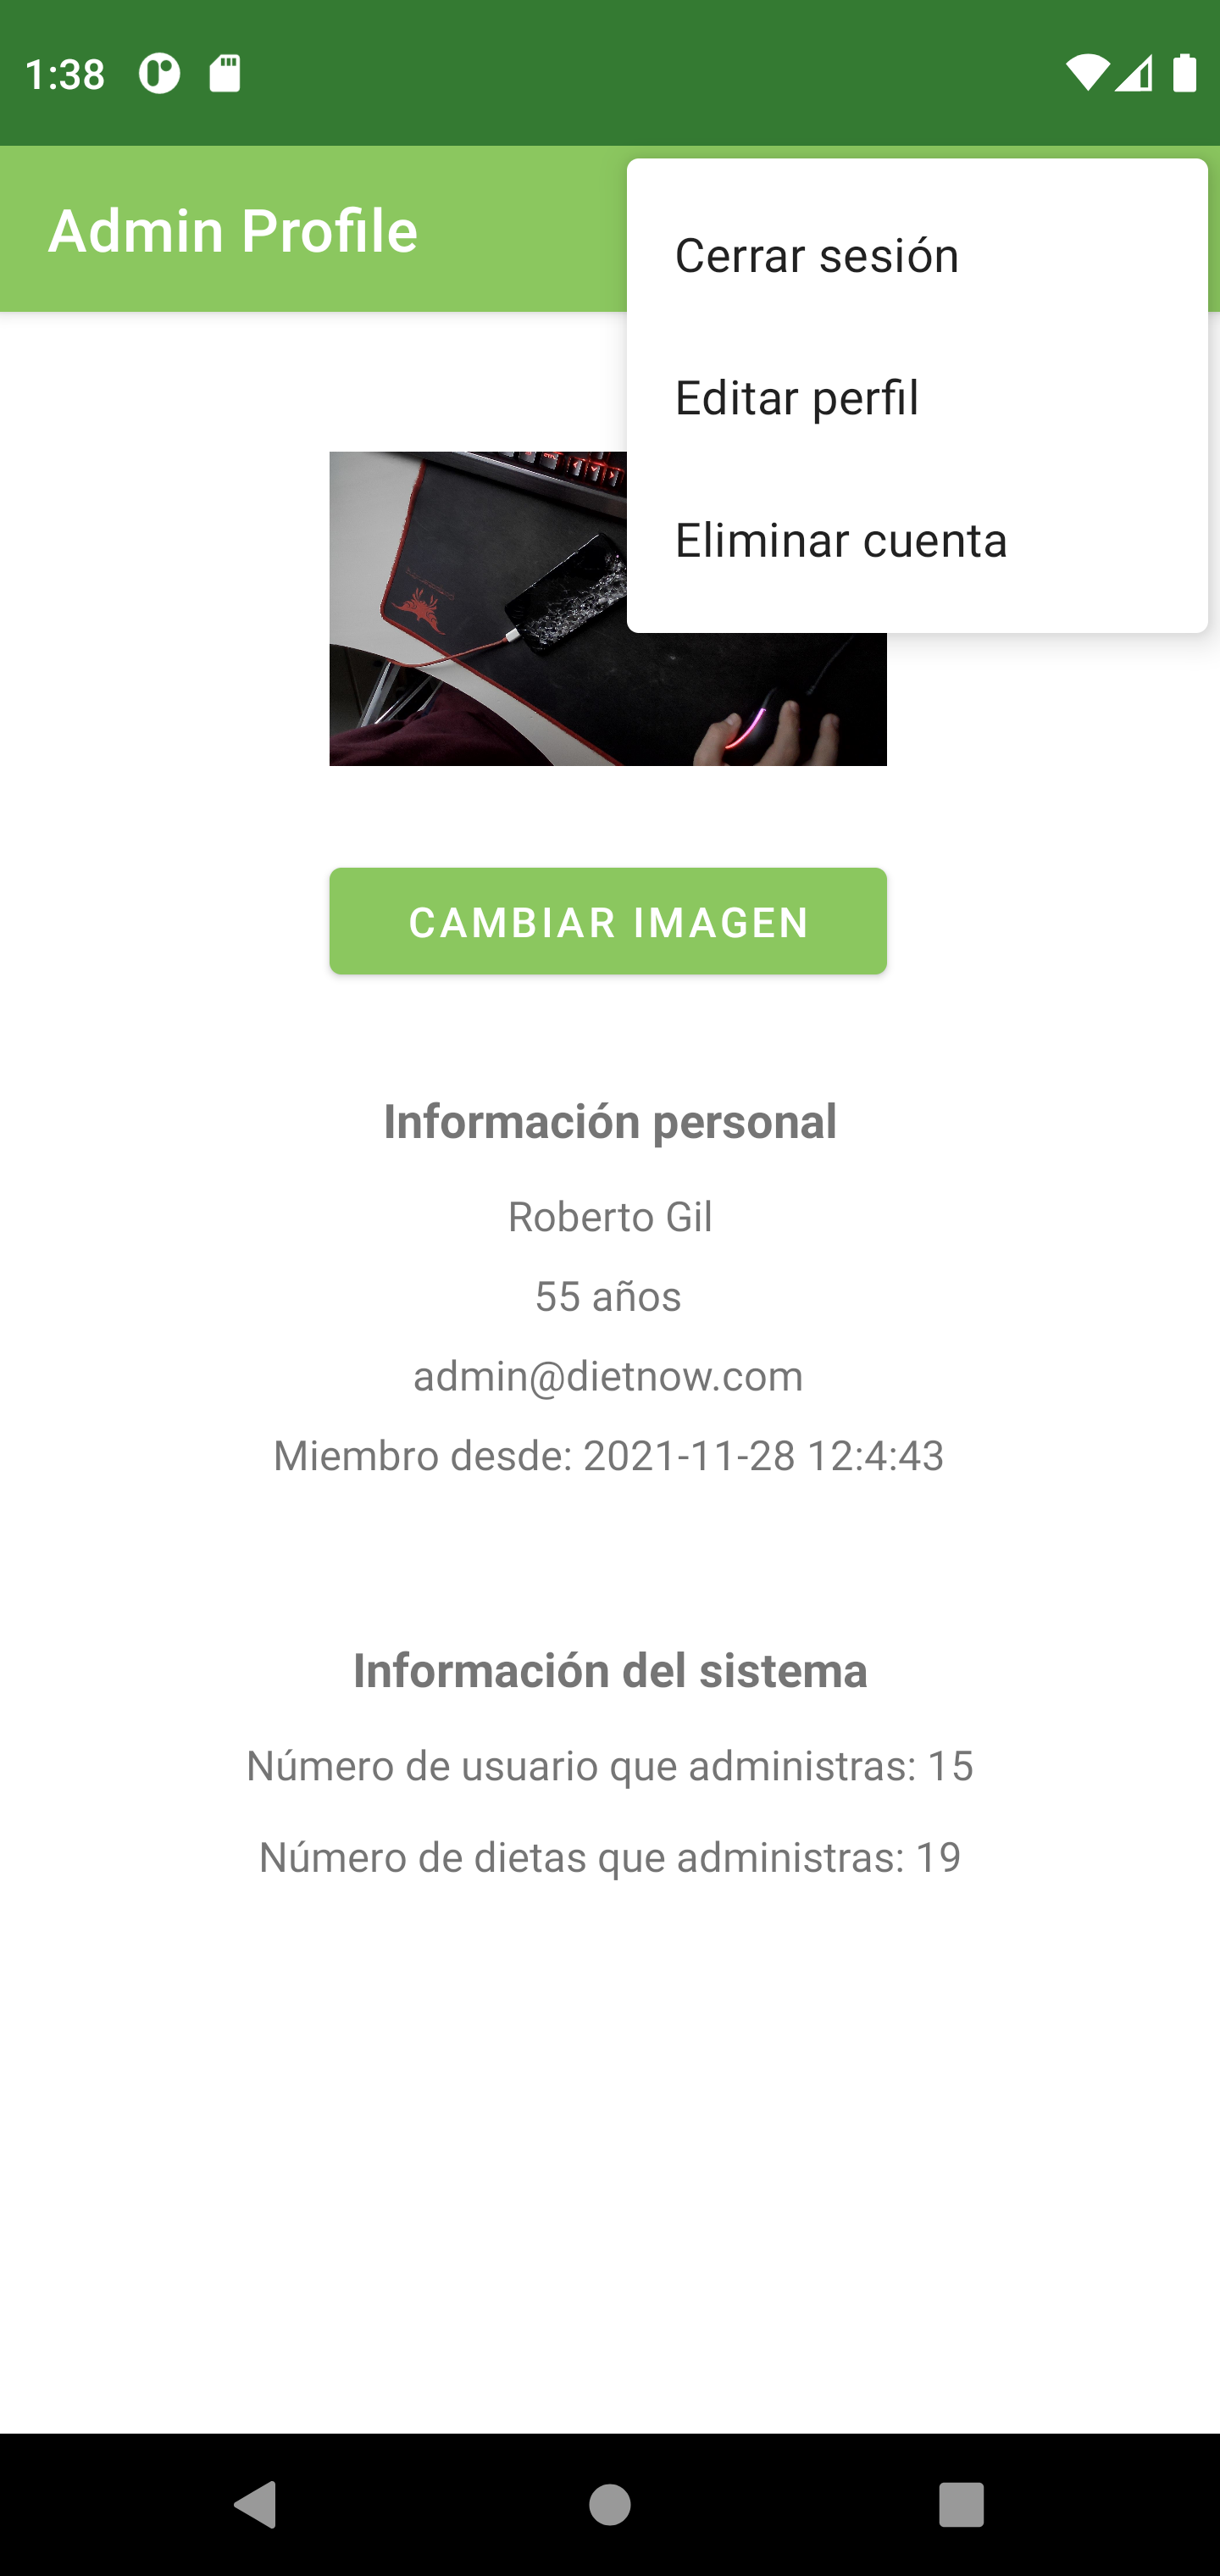
\includegraphics[width=0.4\textwidth]{Images/Annexes/adminProfile2.png}}
    \caption{Vista de ver perfil de un administrador}
    \label{fig:admin_profile}
\end{figure}
% RESETEAR LOS CONTADORES PARA LOS ANEXOS
\setcounter{chapter}{3}
\setcounter{section}{0}
\setcounter{figure}{0}
%%%%%%%%

\anx{II}{Preguntas de la evaluación}
\noindent
En este último anexo se muestran todos los módulos de las preguntas realizadas a los diferentes usuarios que han probado y evaluado la aplicación.

\begin{figure}[H]
    \centering
    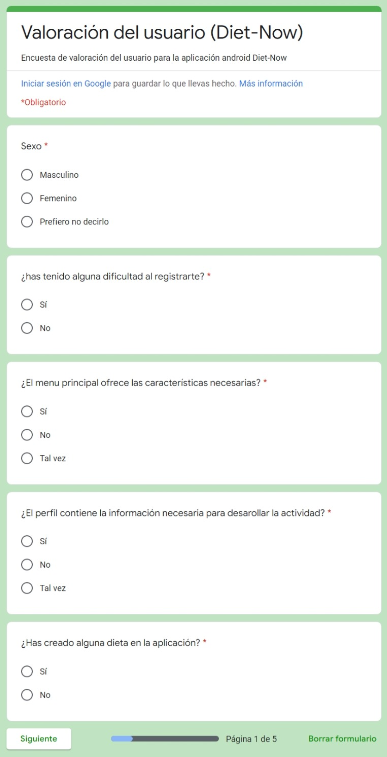
\includegraphics[width=0.75\textwidth]{Images/Capitulo8/Capitulo8.1/val1.png}
    \caption{Preguntas de valoración del usuario}
    \label{fig:preguntas_form_1}
\end{figure}

\begin{figure}[H]
    \centering
    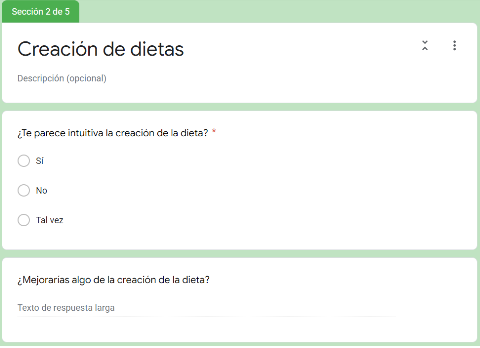
\includegraphics[width=0.75\textwidth]{Images/Capitulo8/Capitulo8.1/val2.png}
    \caption{Preguntas de valoración de creación de dietas}
    \label{fig:preguntas_form_2}
\end{figure}

\begin{figure}[H]
    \centering
    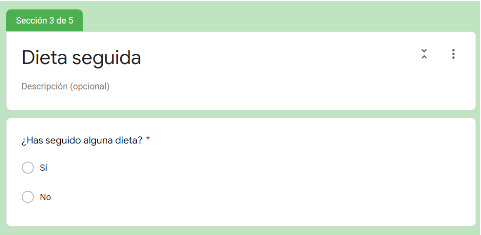
\includegraphics[width=0.75\textwidth]{Images/Capitulo8/Capitulo8.1/val3.png}
    \caption{Preguntas de valoración de dieta seguida}
    \label{fig:preguntas_form_3}
\end{figure}

\begin{figure}[H]
    \centering
    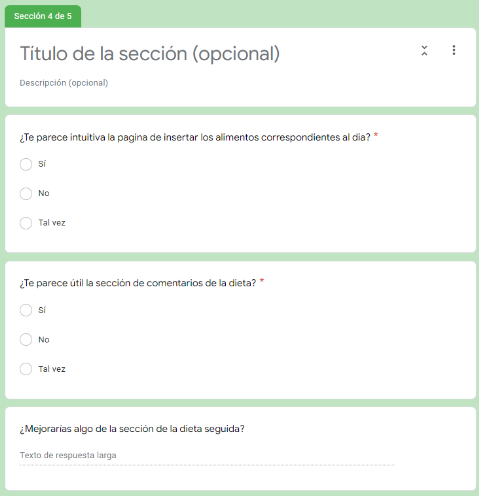
\includegraphics[width=0.75\textwidth]{Images/Capitulo8/Capitulo8.1/val4.png}
    \caption{Preguntas de comentarios sobre la aplicación}
    \label{fig:preguntas_form_4}
\end{figure}

\begin{figure}[H]
    \centering
    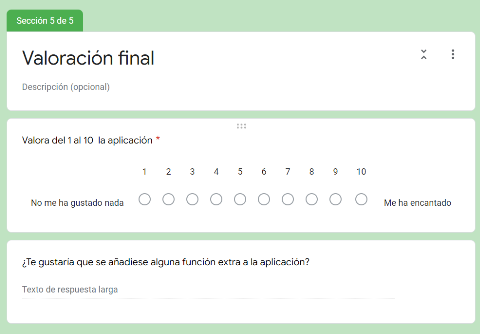
\includegraphics[width=0.75\textwidth]{Images/Capitulo8/Capitulo8.1/val5.png}
    \caption{Preguntas de valoración final de la aplicación}
    \label{fig:preguntas_form_5}
\end{figure}

\licenciaTFG{\hill{``\textit{Todo lo que tenemos que decidir es qué hacer con el tiempo que se nos da}``}{Gandalf}
David Fernández Alejo, Vitaliy Savchenko, Carlos Segundo Nieto, Víctor Velasco Arjona}{Lunes 30 de mayo de 2022}{CC-BY-NC-ND}

%%%%%%%%%%%%%%%%%%%%%%%%%%%%%%%%%%%%%%%%%%%
\end{document}